%%%%%%%%%%%%%%%%%%%%%%%%%%%%%%%%%%%%%%%%%%%%%%%%%%
% 载入模版
%
% 载入csuthesis.cls文件定义的模板
% 支持选项,forprint(黑白打印模式)
% 载入主体内容样式与参考文献样式
%%%%%%%%%%%%%%%%%%%%%%%%%%%%%%%%%%%%%%%%%%%%%%%%%%
% 选项
%   type=[bachelor|research|translation],                  % 可选(默认:bachelor),论文类型(学位or课程/调研报告/文献翻译)
%   output=[print|electronic],                            % 可选(默认:print),输出要求(电子版/打印)
\documentclass[type=bachelor, output=electronic, fontset=none]{csuthesis}
% 来自https://github.com/hushidong/biblatex-gb7714-2015
% 参考文献 gb7714-2015 支持宏包
% 使用了biblatex-gb7714-2015宏包,指定后端为biber
\usepackage[backend=biber,style=gb7714-2015,gbnamefmt=uppercase,gbpub=false,gbpunctin=false]{biblatex}
% 重定义参考文献字体为楷体GB_2312 字号5号
\renewcommand{\bibfont}{\zihao{5} \kgb}
% 导入参考文献数据库
\addbibresource{csuthesis_main.bib}
% 按照章节(chapter)标注图片和表格序号,亦可根据需要改为section等
\counterwithin{figure}{chapter}
\counterwithin{table}{chapter}

% 公式、图片、表格序号改成(1-1)的形式
\renewcommand{\theequation}{\thechapter-\arabic{equation}}
\renewcommand\thefigure{\arabic{section}-\arabic{figure}}
\renewcommand\thetable{\arabic{section}-\arabic{figure}}

% 各级小标题前后间距:前后各一个字符,首行缩进俩字符
% \titlespacing{\section}{0pt}{2.5ex plus 1ex minus .2ex}{1.3ex plus .2ex}
% \titlespacing{\section}{2em}{*0.5}{*0.5}
% \titlespacing{\subsection}{2em}{*0}{*0}

%%%%%%%%%%%%%%%%%%%%%%%%%%%%%%%%%%%%%%%%%%%%%%%%%%
% 基本信息
%
% 用户自行输入标题、作者等基本信息
% 都存储在\content\info.tex文件中
%%%%%%%%%%%%%%%%%%%%%%%%%%%%%%%%%%%%%%%%%%%%%%%%%%
%!TEX root = ../csuthesis_main.tex
% 文章信息
\titlecn{用于水下运输的遥控运载机器人的建模和仿真}
\titleen{Modeling and Simulation of Remotely Operated Carrier Robots for Underwater Transportation}

\priormajor{交通设备与控制工程}     % 主修
\minormajor{}       % 辅修(选填)
\interestmajor{}  % 兴趣(选填)
\author{欧宇恒}              % 作者
\supervisor{阳劲松$\,$副教授}        % 指导老师
\subsupervisor{}
\department{交通运输工程学院}         % 学院
\studentid{8212210728}          % 学号
\thesisdate{year=2025,month=3}  % 时间
\myclass{交设2105班}        % 班级




\begin{document}
%%%%%%%%%%%%%%%%%%%%%%%%%%%%%%%%%%%%%%%%%%%%%%%%%%
% 封面绘制
%
% 1.5版本重新编写了封面绘制宏,并用latex使用者更习惯的
% \maketitle代替之前的\makecoverpage
%%%%%%%%%%%%%%%%%%%%%%%%%%%%%%%%%%%%%%%%%%%%%%%%%%
\maketitle

% 启用大罗马字母进行编号
\frontmatter
% 设置页眉和页脚


%%%%%%%%%%%%%%%%%%%%%%%%%%%%%%%%%%%%%%%%%%%%%%%%%%
% 中文摘要
%
% 存储在\content\abstractzh.tex文件中
%%%%%%%%%%%%%%%%%%%%%%%%%%%%%%%%%%%%%%%%%%%%%%%%%%
%!TEX root = ../csuthesis_main.tex
% 设置中文摘要
\keywordscn{参数辨识\quad 扩展卡尔曼滤波\quad MPC控制算法}
%\categorycn{TP391}
\begin{abstractzh}

随着“海洋强国”的发展,海底运输、海底勘探越来越成为全球性的热门研究问题,近年来,水下机器人由于其灵活性和可控的自主性而被广泛应用于水下运输、海底探测等专业领域,本文针对用于水下运输的遥控运载机器人进行建模和仿真研究。

本文的研究对象为BlueROV2这款开源机器人,根据BlueROV2的相关结构特性,定义运动参数,建立载体坐标系和惯性坐标系,获得运动学方程,又根据水下环境和BlueROV2电机分布对水下机器人进行受力分析,得到动力学方程。随后,本文将BlueROV2的六自由度运动解耦为水平面运动模型和竖直面运动模型,分别对两个运动模型设计最小二乘算法,辨识出水动力系数;此外,为解决各个自由度之间的强耦合关系,设计基于扩展卡尔曼滤波器(EKF)的辨识算法,搭建包含控制系统、测量系统的仿真结构,对水动力系数进行辨识。最后,本文通过UUV Simulator搭建水下环境和MPC控制框架,设计圆形和双纽线形轨迹跟踪任务,分别验证最小二乘算法和EKF算法辨识出的参数在轨迹跟踪任务下的表现,得出结论,圆形轨迹下,EKF算法较最小二乘算法表现更好,而双纽线轨迹下,两种算法的轨迹追踪任务表现相当。


\end{abstractzh}

%%%%%%%%%%%%%%%%%%%%%%%%%%%%%%%%%%%%%%%%%%%%%%%%%%
% 英文摘要
%
% 存储在\content\abstracten.tex文件中
%%%%%%%%%%%%%%%%%%%%%%%%%%%%%%%%%%%%%%%%%%%%%%%%%%
%!TEX root = ../csuthesis_main.tex
\keywordsen{System Identification\ \ Extended Kalman Filter\ \ MPC Controller}
\begin{abstracten}

With the development of a "maritime power", underwater transportation and seabed exploration have increasingly become hot research topics. In recent years, underwater robots have been widely applied in professional fields due to their flexibility and controllable autonomy. This paper conducts modeling and simulation research on the Remotely Operated Vehicle (ROV) used for underwater transportation. 

The subject of this paper is the open-source robot BlueROV2. Based on the relevant structural characteristics of BlueROV2, we define the motion parameters, establish the inertial frame and body-fixed frame, and obtain the kinematic equations. Then, we analyze the force analysis of the underwater robot with the underwater environment characteristics and the motor distribution of BlueROV2, and finally, obtain the dynamic equations. Subsequently, the six-dofs motion of BlueROV2 is decoupled into the horizontal motion model and the vertical motion model. The least squares algorithm is designed for the two motion models to identify the hydrodynamic coefficients. In addition, to solve the strong coupling relationship among the degrees of freedom, an identification algorithm based on the extended Kalman filter (EKF) is designed, and a simulation structure including the control system and the measurement system is built to identify the hydrodynamic coefficients. Finally, the underwater environment and the MPC control framework are built in UUV Simulator, which is a simulation tool based on ROS and Gazebo. We design the circular and lemniscate trajectory tracking tasks to verify the different performance between the two parameter groups, identified by the LS and EKF, respectively. The conclusion is drawn that the EKF algorithm performs better than the least squares algorithm in the circular trajectory, while the performance of the two algorithms in the lemniscate trajectory tracking task is comparable.

\end{abstracten}


%%%%%%%%%%%%%%%%%%%%%%%%%%%%%%%%%%%%%%%%%%%%%%%%%%
% 目录
%
% 使用重定义的tableofcontents宏绘制目录
% 满足学校的样式要求
%%%%%%%%%%%%%%%%%%%%%%%%%%%%%%%%%%%%%%%%%%%%%%%%%%
\tableofcontents


% 启用数字编号,改为第 x 页  共 x 页格式
\mainmatter

%%%%%%%%%%%%%%%%%%%%%%%%%%%%%%%%%%%%%%%%%%%%%%%%%%
% 正文
%
% 存储在\content\content.tex文件中
%%%%%%%%%%%%%%%%%%%%%%%%%%%%%%%%%%%%%%%%%%%%%%%%%%
% 正文
%!TEX root = ../csuthesis_main.tex

%子章节为了便于查找和修改,建议通过input拆分文件

%%%%%%%%%%%%%%%%%%%%%%%%%%%%%%%%绪论%%%%%%%%%%%%%%%%
%!TEX root = ../../csuthesis_main.tex
\chapter{绪论}

\section{研究背景及意义}
随着人类社会与科技的飞速发展,对广袤海洋的认知、开发与利用已成为衡量国家综合国力的重要标志,并以前所未有的速度向深远海拓展。海洋不仅是地球上最大的资源宝库,蕴藏着丰富的生物、矿产(石油、天然气、可燃冰、多金属结核等)和可再生能源,更是关乎全球气候、生态平衡和国家战略安全的关键领域。在提出“海洋强国”的当下,高效、可靠的水下交通、运输、探测与作业能力成为关键支撑。

特别是对于蕴藏着丰富战略资源的深海区域,实现有效抵达和精细作业是进行科学考察、资源勘探、环境监测以及海底设施(如管线、电缆、观测网)布放与维护等活动的前提。传统的载人潜水器虽然能够执行部分任务,但面临着生命支持系统复杂、作业时间受限、以及对潜航员生理和心理的巨大考验等问题,尤其是在高压、黑暗、低温的极端深海环境中,其风险和成本居高不下。因此,发展和应用能够替代或辅助人类在水下执行复杂任务的无人化装备,已成为国际海洋工程技术发展的重要趋势。

由水下机器人承载起的水下交通对于深海的探测工作具有重要意义。广袤的海洋,尤其是深远海,人类难以直接进入。水下运载平台的运输能力,使得搭载着探测传感器的系统能够克服水深、压力、黑暗等障碍,抵达遥远、未知或危险的水下区域。水下平台的机动性、多传感器的感知能力、自适应控制的导航和避障能力,使其能够按照预定路径或自适应路径进行移动,对大面积海域或海底进行系统性的扫描和测绘,如海底地形地貌勘测、管线巡检、资源普查等,丰富了探测范围与探测能力。\cite{CaiWeiZiZhuShuiXiaJiQiRenHaiDiReYeQuYingYongZongShu2023}

为了克服水下环境的限制,各类水下机器人应运而生,主要包括遥控水下机器人(Remotely Operated Vehicle, ROV)和自主水下机器人(Autonomous Underwater Vehicle, AUV)。ROV通过线缆与母船连接,由操作员远程控制,具有实时监控、精确操作和强作业能力的优点,广泛应用于海底观测、资源勘探、管线检查、水下结构物安装与维护、沉船打捞、水产养殖等领域。随着水下任务复杂度的提升,特别是涉及物品搬运、设备部署、样品采集与回收等需求的增加,对具备水下运输能力的ROV提出了更高的要求。

水下遥控运载机器人(Remotely Operated Vehicle, ROV),作为一种通过脐带缆从母船获取动力和传输控制/数据信号的无人潜水器,能够搭载多种传感器和作业工具,凭借其操作灵活、作业时间长、环境适应性强等优势,在这一需求下应运而生并扮演着越来越重要的角色。ROV在水下运动时,其动力学行为受到自身结构、流体介质以及所携带载荷的复杂耦合影响,包括非线性的水动力(流体阻力、附加质量效应等)、科里奥利力、重力与浮力变化、推进器推力特性以及环境干扰(如洋流)等。当ROV携带不同形状、尺寸和质量的载荷时,其整体的惯性特性和水动力特性会发生显著变化,这使得建立一个能够精确描述其运动行为的动力学模型成为一大难题。

更为关键的是,模型中的许多核心参数,特别是描述流体与机器人相互作用的“水动力系数”(如阻尼系数、附加质量系数),往往难以通过纯理论计算精确获得,且可能随工作状态和环境变化而改变。因此,仅仅建立理论模型是不够的,必须通过有效的方法对这些关键参数进行动态辨识。通过分析ROV实际运行(或高保真仿真)过程中的运动状态数据,包括导航轨迹、速度、加速度等,结合参数辨识算法,实时反推出准确的水动力系数,才能获得真正贴合实际工况的高精度动力学模型。这对于后续设计能够适应载荷变化和环境扰动的高性能控制器至关重要。

在拥有了经过辨识校准的精确动力学模型之后,需要实现一个高保真的仿真平台和控制器,通过机器人跟踪预设路径的实际效果以验证动力学模型的辨识表现。在物理样机制造和昂贵的水池试验之前,高保真仿真平台可以对ROV的机械结构、推进器配置、传感器布局等设计方案进行快速迭代和评估,能够测试和验证导航、制导与控制(NGC)算法,以及图像处理、路径规划等上层智能算法,而无需担心损坏真实ROV或应对复杂的实际测试准备。此外,高保真仿真平台可以轻易地改变水动力参数、质量分布等,可以研究这些参数对ROV运动性能的影响,加深对ROV动力学特性的理解。

综上所述,用于水下运输的遥控运载机器人的建模和仿真,旨在深化对载荷变化下水下机器人复杂动力学行为的理解,探索将先进优化算法应用于水动力参数动态辨识的有效途径,并深入研究模型预测控制在解决此类强非线性、多约束、时变系统高精度轨迹跟踪问题上的应用潜力与理论方法。有望显著提升水下运输机器人的轨迹跟踪精度、作业稳定性以及对变化的载荷与环境的适应能力,为“海洋强国”战略的实施提供关键技术支撑和人才储备。

\section{水下机器人分类}

常见的水下机器人可根据其外形结构、工作情景与应用范围分为三类:遥控式水下机器人,载人潜水器,自治水下机器人。

遥控潜水器 (Remotely Operated Vehicle,简称ROV) 是一种无人水下机器人,其携带有一根长电缆,通过这根电缆传送能源和信号。操作者可以通过这根电缆对机器人进行遥控操作。ROV的优点是能够在一个小范围内精细的观测,可以携带机械手和作业工具在海底进行精细取样作业,比如采集岩石、海底沉积物,收集失落在海底的物体,取水样、泥样等。

载人潜水器(Human Occupied Vehicle,简称 HOV),是一种可以携带研究人员的大型水下航行器。HOV 可由内部潜水器内部的研究人员进行操纵,具有较强的水下作业能力。HOV 不是完全自主运动的,需要母船进行氧气以及能源的补给,因此航程一般较短。

自治水下机器人(Autonomous Underwater Vehicle,简称 AUV),是一种完全自主的无人式水下机器人。AUV 在下水之前就已经被写入相关控制程序,可以按照预先设置好的控制策略进行自主航行,具有较高的智能水平。

\section{国内外研究现状}
\subsection{ROV建模与仿真技术研究现状}
水下机器人动力学建模是利用物理学原理,来建立描述机器人运动状态,如位置、姿态、速度和加速度)与其所受各种力及力矩之间关系的数学模型。建立水下机器人动力学模型的核心目标是深入理解机器人在复杂水下环境中的行为规律,并能够预测其在不同驱动力和环境干扰下的运动响应。建立精确的动力学模型对于后续的控制系统设计至关重要,因为它为控制器提供了计算所需驱动力以实现期望运动的基础。同时,该模型也是进行仿真测试、验证算法、优化机器人设计以及辅助导航状态估计的关键工具。在建模过程中,需要综合考虑机器人的刚体惯性效应、复杂的水动力效应、静水恢复力、推进系统的推力特性,以及来自水流、波浪或缆绳等外部环境的干扰力。最终,动力学模型通常表现为一套耦合的、非线性的六自由度(6-DOF)常微分方程组,它系统地刻画了水下机器人在力和力矩作用下的完整动态响应特性。

近几十年来,世界各地的研究人员针对ROV动力学建模进行大量研究工作,许多经典的动力学建模方法被工程应用。现阶段使用较多的动力学建模方法是将ROV视为刚体,对ROV进行受力分析,从而通过刚体动力学理论建立动力学模型。国内李殿璞学者\cite{LiDianPuChuanBoYunDongYuJianMo2008}用牛顿-欧拉法推导了水下航行器动力学模型的一般表达式,将水下航行器的动力学分解为水平面水动力与垂直面水动力,分别推导表达式;挪威学者Fossen系统地提出了ROV的流体动力学模型\cite{fossenHandbookMarineCraft2021},现该模型已经被广泛使用在ROV运动控制领域,成为该领域内的标准模型;我国孙元泉、马运义等人\cite{2001潜艇和深潜器的现代操纵理论与应用}也对水下航行器进行建模研究,将水下航行器建模进一步划分为垂直面操纵模型和水平面操纵模型;Malte von Benzon等\cite{vonbenzonOpenSourceBenchmarkSimulator2022}在Fossen模型的基础上,使用集中质量法对连接ROV和顶部设施的系绳进行了建模,并将其作为ROV模型的力输入。

在建立 AUV 的理论模型之后,不同几何特征与应用场景的 AUV 需要通过实验方法进行计算获得具体的模型参数。水下航行器由于其处于非结构性环境下,水域情况复杂,难以用简单的数学公式精确描述,环境干扰对系统影响大,无法求得动力学模型参数的解析解。除此之外,ROV为了搭载各种传感器和作业工具,外形通常不是理想的流线型,这导致了复杂的流场环境,使得水动力特性更加难以求解。

有许多学者水动力参数的辨识方法进行研究,对于水动力参数辨识的方法主要分为:实验数据驱动法、模型拟合法、数值计算法(CFD)。在实验数据驱动法中,Massimo Caccia\cite{cacciaModelingIdentificationOpenframe2000}通过收集传感器数据,利用最小二乘法先后辨识了阻力和推进器安装系数与系统惯性矩阵;Eschmann等\cite{eschmannDataDrivenSystemIdentification2024}利用机体传感器数据辨识四旋翼飞行器的惯性参数、推力曲线、力矩系数和一阶电机延迟,以此完善飞行器动力学模型,该方法可以被借鉴到水下机器人的辨识过程中;Deng等人\cite{dengIdentificationAutonomousUnderwater2021}比较了无迹卡尔曼滤波、扩展卡尔曼滤波和时域离散优化卡尔曼滤波器三种滤波算法在辨识水动力参数上的准确性,提出了自回归滑动平均( ARMA )噪声模型以提高估计精度和扰动抑制性能。模型拟合法提供了一种数据驱动的方法,可以直接从ROV的实际运动数据中提取这些关键参数,其中,Zohedi\cite{zohediSYSTEMIDENTIFICATIONSI2023}、Aras\cite{arasThrusterModellingUnderwater2013}等采用MATLAB Simulink的系统辨识工具箱,选择合适的模型拟合ROV系统运动轨迹,用于控制ROV悬浮状态的稳定性。数值计算法中,Zhang\cite{zhangStudyImpactProcess2017}、Zheng\cite{zhengStudyHydrodynamicPerformance2017}等人利用计算流体动力学的方式,利用商业软件GAMBIT或FLUENT建立网格和划分流域,对不同工况结果进行仿真求解,获得水动力系数较为容易,但其求解结果十分依赖于网格设置精度。

\subsection{ROV仿真平台研究现状}

随着技术的发展,仿真平台技术突飞猛进,被广泛使用在ROV的研发过程中。水下机器人仿真平台是一种利用数字化技术实现水下环境与机器人的虚拟再现的重要工具,能够有效支持算法开发、任务规划及环境感知等多方面的研究与实践\cite{cookSurveyAUVRobot2014}。其核心目的是通过虚拟环境代替真实场景进行实验和测试,以降低实验风险和成本,同时提高算法开发效率和仿真结果的可控性。当前主要的ROV仿真平台如下:

\subsubsection{Gazebo}

Gazebo 是一款功能强大的开源 3D 物理仿真引擎,在机器人学研究和开发中得到了广泛应用。其可以与机器人操作系统(ROS)结合,支持通过特定插件包进行扩展,实现各项高保真仿真功能,主要包括:1)动力学仿真:Gazebo 支持多种高性能的物理引擎,如 ODE、SimBody、ART、Bullet 等。用户可以在机器人模型三维模型文件的基础上设置机器人及周围环境的物理;2)可视化三维流体环境:用户可以创建或导入复杂的海底地形、水下结构物(如管道、沉船、平台)、珊瑚礁等三维模型,构建逼真的水下作业场景;3)流体仿真:引入流体动力学模型,模拟水下机器人在流体中的运动响应;4)视觉开发:模拟水下光学图像,可以调整水体浑浊度、光照等参数,用于视觉导航、目标识别算法的开发。

\subsubsection{DAVE}

DAVE是一个构建水下机器人仿真环境的开源功能包。DAVE 的核心设计理念是高度模块化。它旨在提供一个框架,用户可以像搭积木一样组合不同的软件模块来快速构建和仿真各种类型的水下航行器及其任务。除此之外,DAVE 提供了丰富的用于实现机器人行为和任务逻辑的框架,包括航向保持、深度保持、速度保持、航点跟踪,其允许用户定义一系列任务或目标,并让机器人自主执行。更侧重于水下机器人自主行为的模块化设计、任务级控制和决策逻辑的快速原型验证。它的物理仿真和渲染可能不如Gazebo精细,但其组件化架构在构建和测试复杂自主系统方面有优势。

\subsubsection{MATLAB/Simulink}

MATLAB/Simulink 是工程领域广泛使用的数学计算和基于模型的设计环境,在水下机器人仿真中也扮演着非常重要的角色。它们提供了一套强大而灵活的工具,用于水下机器人的建模、控制系统设计、算法开发和仿真分析。MATLAB/Simulink 提供了多种控制系统设计工具箱,支持设计和调试PID控制器,并进行参数整定;设计和仿真MPC控制器,能够处理约束和优化性能指标。但其物理真实感和3D渲染比不上专业物理仿真引擎;对于复杂的水下环境的模拟能力有限,对于模拟传感器的物理感知过程较为粗糙。

\subsection{ROV运动控制技术研究现状}

水下机器人的控制器设计与轨迹跟踪是实现其自主或遥控作业能力的核心环节,确保机器人能够精确、稳定地按照预定的路径或指令运动。控制器根据机器人的当前状态与期望状态之间的误差,计算出需要施加给推进器系统的控制指令。这个过程必须克服水下环境带来的巨大挑战,包括机器人自身复杂的非线性、强耦合动力学特性,难以精确建模的水动力参数及其时变性,以及无处不在的外部干扰,如未知的水流、波浪影响等。轨迹跟踪要求控制器不仅要使机器人到达某个点,更要使其在运动过程中紧密地、平滑地跟随一条在空间和时间上都已定义好的路径。为了实现有效的轨迹跟踪,研究人员开发了多种控制策略。

\subsubsection{PID控制}

PID(Proportional-Integral-Derivative,比例-积分-微分)控制器是一种在工业控制应用中常见的反馈控制器。它的核心思想是根据被控对象的期望值与实际输出值之间的误差,通过比例、积分、微分三种运算的线性组合来产生控制信号,驱动执行机构,从而使实际输出值趋近期望值。简单的PID(比例-积分-微分)\cite{liuUnderwaterRemotelyOperated2023}控制因其结构简单、易于实现而被广泛应用\cite{zohediSYSTEMIDENTIFICATIONSI2023},但在面对强非线性和显著不确定性时往往性能受限,需要对PID控制进行改进或者与其他控制策略复合控制,包括神经网络自回归PID控制\cite{hernandez-alvaradoNeuralNetworkBasedSelfTuning2016},模糊PID控制\cite{dongDepthControlROV2020a},结合改进粒子群优化算法PID控制\cite{liuUnderwaterRemotelyOperated2023a}。

\subsubsection{滑模控制}

滑模控制是一种非线性鲁棒控制方法,其核心思想是将系统的控制问题分解为两个阶段,在到达阶段上,需要设计一个控制律,使得系统的状态轨迹能够在有限时间内到达并保持在一个预先设计好的切换超曲面上,这个超曲面也称为滑模面; 一旦系统状态轨迹到达滑模面上,控制律将迫使状态轨迹沿着该滑模面滑动,进入滑动阶段,并最终趋向于平衡点,滑模控制因其对模型不确定性和外部干扰的强鲁棒性而被广泛应用于水下机器人领域\cite{renROVSlidingMode2023},Chen等\cite{chenFunctionbasedRobustSliding2025}将滑膜控制与干扰观测器相结合,用于解决ROV抖振与动力学模型不确定性问题;Bessa等\cite{bessaDepthControlRemotely2008}通过自适应模糊算法与滑膜控制算法相结合来增强不确定性干扰补偿,在保证消除抖振的同时实现了光滑的曲线跟踪。

\subsubsection{基于智能算法的自适应控制}

随着计算机技术和人工智能的发展,智能算法,如神经网络、模糊逻辑、遗传算法、粒子群优化、强化学习等被越来越多地引入到自适应控制领域,形成了基于智能算法的自适应控制。这种结合被认为是控制领域的一个先进发展方向,因为它能够克服传统自适应控制的一些局限性,并为处理更复杂、更不确定的系统提供了新的思路和工具。Bagheri等\cite{bagheriTrackingPerformanceControl2010}利用自适应神经网络控制有效提升了水下机器人的轨迹跟踪性能;Chu等\cite{chuObserverBasedAdaptiveNeural2017}提出了基于局部RNN的自适应终端滑模状态观测器,以保证轨迹跟踪误差在有限时间内得以收敛,提高了轨迹跟踪的精度和稳定性。

\subsubsection{模型预测控制(MPC)}

模型预测控制(MPC)将ROV的动力学模型纳入控制流程中,该方法利用已建立的、尽可能精确的ROV动力学模型预测系统在未来一段时间内对一系列候选控制输入序列的响应。基于这些预测结果,MPC通过求解一个在线优化问题,寻找能够在预测时域内最小化预定性能指标并同时满足各种物理约束的最优控制输入序列,相比那些不直接进行基于模型预测优化的控制器,往往能实现更优的控制性能和对未来行为的主动管理。Shen等\cite{shenTrajectoryTrackingControl2018}提出基于李雅普诺夫的模型预测控制器,优化了闭环控制系统的稳定性;Hu等\cite{huDisturbanceObserverBasedModel2024}将扩张主动观测器与模型预测控制相结合,用于处理ROV的外部信号干扰和模型噪音,有效屏蔽了外部不可预测的干扰信号;Hu等将MPC控制与扩展主动状态观测器相结合,与传统的干扰观测器相比,所开发的算法具有同时处理外部干扰和系统测量噪声的能力。

\section{论文组织结构}

本文主要研究了用于水下运输的遥控运载机器人的建模与仿真,首先对水下机器人进行运动学建模和动力学建模,建立ROV运动控制的基础理论,然后提出了基于最小二乘法和扩展卡尔曼滤波器的动力学参数辨识算法,最后通过UUV Simulator仿真系统完成了对ROV运动控制的仿真,并且比较两种算法辨识结果在轨迹跟踪这一任务需求上的优劣。

本文研究内容及分布如图\ref{f.thesis_framework}所示。

\begin{figure}[hbt]
    \centering
    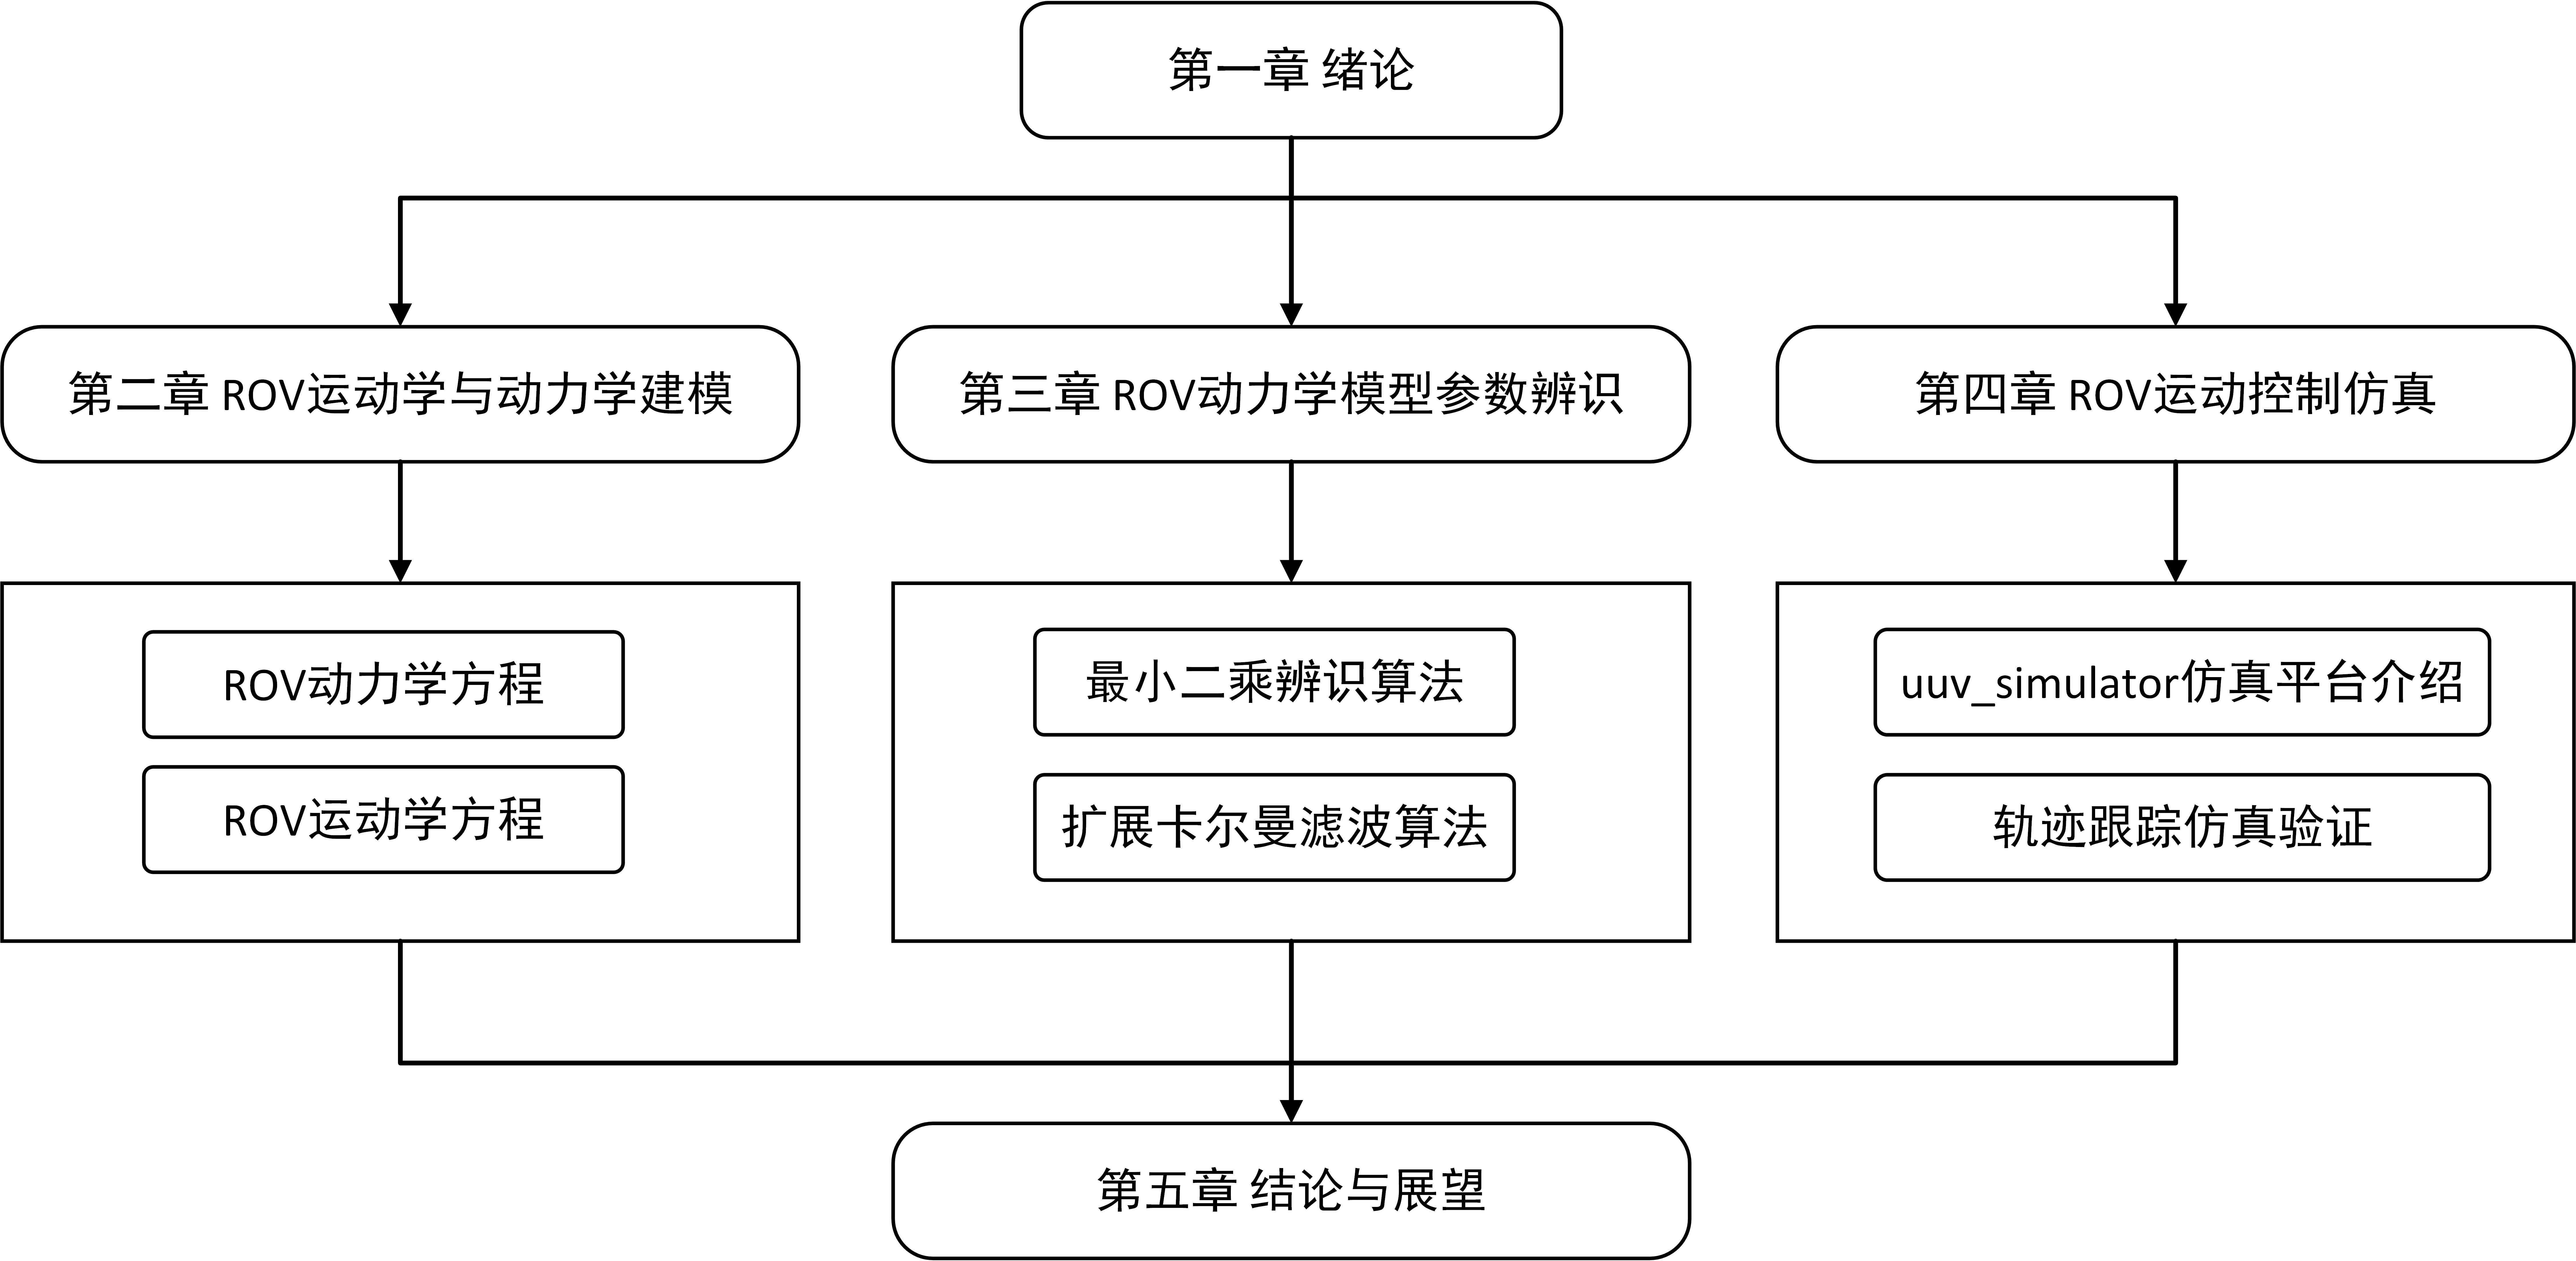
\includegraphics[width=\linewidth]{images/chapter1/论文架构图.png}
    \caption{本文研究结构}
    \label{f.thesis_framework}
\end{figure}

第一章主要介绍了研究课题的背景和意义,介绍了本文研究对象ROV建模与仿真技术、ROV水下运动控制技术在当下国内外的发展现状,并简要阐述了本文的主要研究内容。

第二章主要完成了ROV运动学模型与动力学模型的建立,ROV运动学模型与动力学模型是控制ROV运动的基础。在本章,首先介绍了Bluerov2的主体结构与组成,通过建立相关坐标系、定义相关运动参数以获得ROV运动学方程;通过建立水动力阻尼模型,对ROV进行受力分析,得到ROV的动力学方程。

第三章主要介绍了最小二乘算法与扩展卡尔曼滤波器算法的原理,分别利用其辨识动力学模型的未知参数,完成了动力学模型参数辨识的算法设计,通过MATLAB/Simulink仿真实现了扩展卡尔曼滤波器的参数辨识过程。

第四章主要介绍了UUV Simulator的主要架构,ROV控制器设计,在仿真平台上控制ROV按照预设轨迹运动,并通过修改仿真平台中ROV动力学模型参数,比较最小二乘算法与扩展卡尔曼滤波器算法的辨识效果在轨迹跟踪这一任务上的实际表现,完成了对Bluerov2的轨迹跟踪控制功能。

第五章主要对本文工作进行总结,并对本课题以后的研究方向进行展望。

\newpage
%%%%%%%%%%%%%%%%%%%%%%%%%%%%%%%%绪论%%%%%%%%%%%%%%%%

%%%%%%%%%%%%%%%%%%%%%%%%%%%%%%%%图像插入示例%%%%%%%%%%%%%%%%
%!TEX root = ../../csuthesis_main.tex
\chapter{ROV 运动学与动力学建模}

对于水下遥控机器人(ROV)而言,其运动学模型与动力学模型同样是实现精确运动控制的基础,并且是进行高保真运动控制仿真的先决条件。ROV 运动模型的准确度,直接决定了其运动控制系统的鲁棒性、作业效率以及最终的定位与操纵精度。ROV 的水下运动系统本质上是一个高度非线性、多自由度间强耦合的动态系统,一个精确的动力学模型能够更准确地预测 ROV 在推进器作用下的运动响应,为设计高性能的控制器如姿态保持、轨迹跟踪控制器,提供坚实的基础,从而有效提升 ROV 的自主作业能力、环境适应性和作业效率。

\section{BlueROV2 结构设计介绍}

本课题的研究对象为开源水下机器人 BlueROV2\cite{huDisturbanceObserverBasedModel2024}。BlueROV2 为系留式 ROV,系绳用于车辆与陀螺仪单元之间的通信,航行器既可以通过系绳供电,也可以通过车载电池供电。该 ROV 配备有六个推进器,推进器的相互配合能够完成对 ROV 姿态和运动的控制,ROV 搭载各种车载传感器,包括压力传感器、惯性测量单元、磁力计、激光照相机、探测声呐,可以配合短基线测量技术与多普勒测速仪获取位置和速度状态。其中,IMU 由加速度计和陀螺仪组成,能够测量出 ROV 此时的位姿向量。BlueROV2的构成如图\ref{f.BlueROV2}所示。

\begin{figure}[hbt]
    \centering
    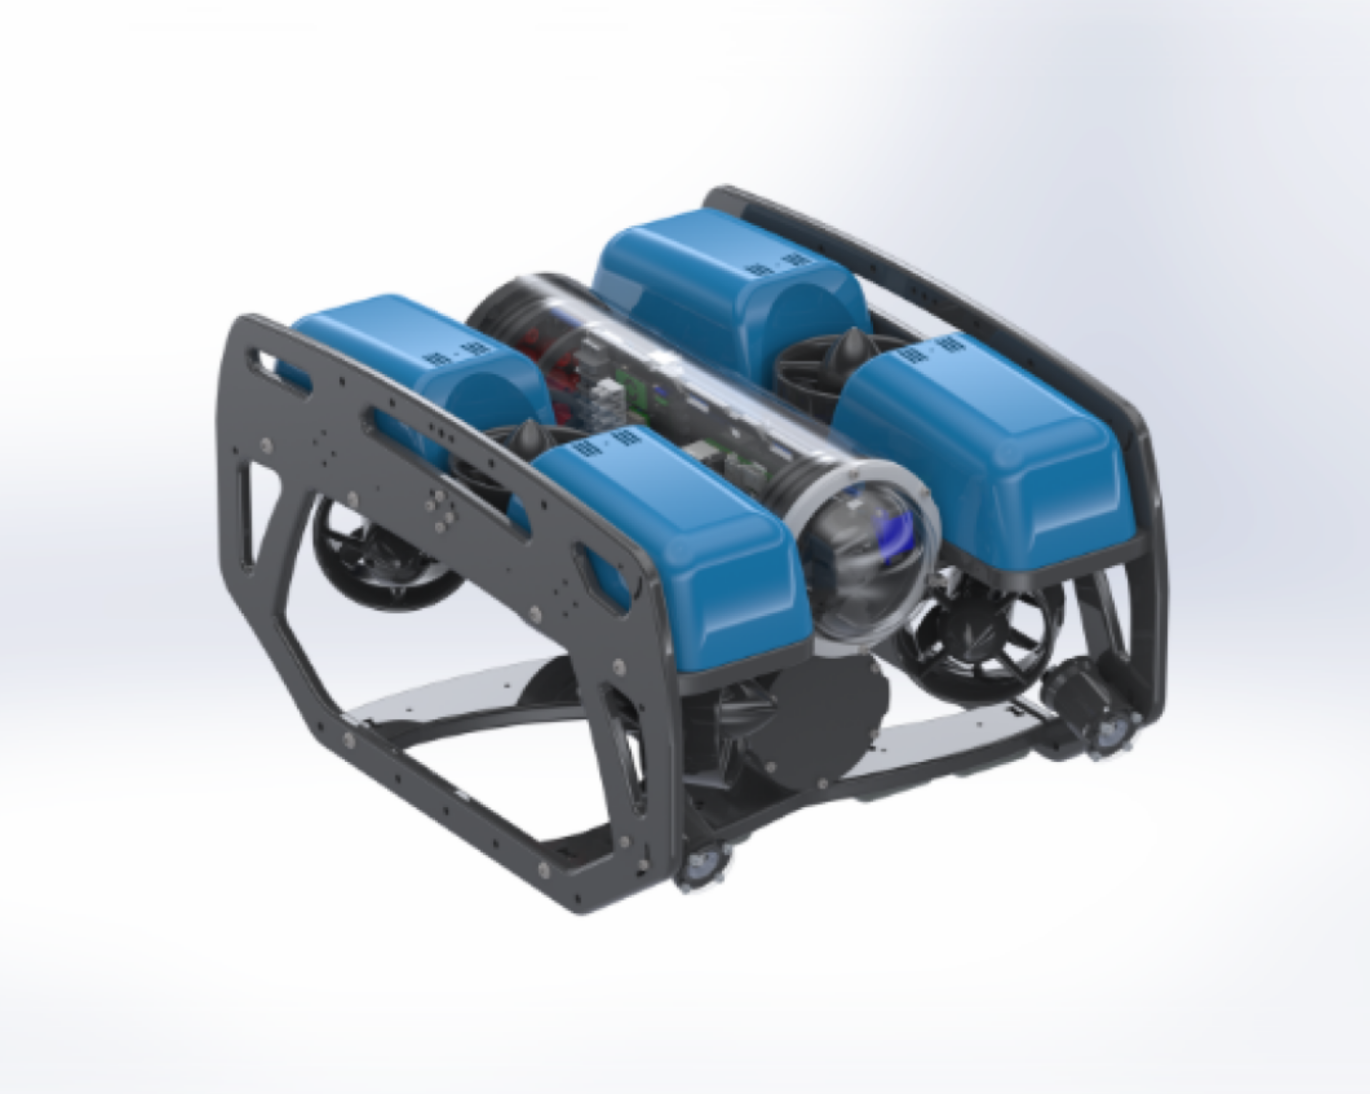
\includegraphics[width=0.6\linewidth]{images/chapter2/bluerov.png}
    \caption{BlueROV2 三维结构}
    \label{f.BlueROV2}
\end{figure}

BlueROV2搭载的传感器可以用于测量系统的状态向量,各传感器技术的测量物理量,采样率和方差如表\ref{t.sensors}所示。
\begin{table}[htb]
  \centering
  \caption{BlueROV2机载传感器参数表}
  \zihao{5}
  
  \label{t.sensors}
  \begin{tabular}{cccc}
  \hline
传感器技术 & 测量状态  & 采样率 & 方差 \\
\hline
压力计 & $z_b$ & 20Hz & $1.5\times 10^{-5}\text{m}$ \\
惯性测量单元 & $\phi, \theta$ & 1000Hz & $1\times 10^{-5}\text{ rad to } 2.5\times 10^{-5}\text{rad}$ \\
磁力计 & $\psi$ & 1000Hz & \multirow{2}{*}{$2\times 10^{-6}\text{m}$} \\
激光照相机 & $x, y$ & 20Hz & \\
短基线技术 & $x_b, y_b$ & 4Hz & $1\times 10^{-3}\text{m}$\\
\hline
\end{tabular}
\end{table}

\section{BlueROV2 运动学建模}
\subsection{坐标系建立与运动参数的定义}

描述 ROV 位置、姿态、速度、加速度之间关系的运动学方程,必须在特定的坐标系下才有意义,用于水下运输的遥控运载机器人的运动可以视为六自由度的运动,一般而言需要建立世界惯性坐标系与运动的载体坐标系用于描述 ROV 的运动参数,两者均满足笛卡尔右手坐标系原则。惯性坐标系的原点取在大地上的一点,Z 轴指向地心,X,Y 轴在水平面内互相垂直,ROV 载体坐标系的原点与 ROV 的重心重合,即:设置 ROV 重心坐标为$r_g=[x_g,y_g,z_g]^T=[0,0,0]^T$,Z 轴指向 ROV 竖直下沉方向,X 轴与 ROV 进退方向平行,指前进方向为正向,Y 轴与 ROV 横移方向平行。根据 BlueROV2 结构,建立惯性坐标系与载体坐标系如图\ref{f.frame_identification}所示。

\begin{figure}[hbt]
    \centering
    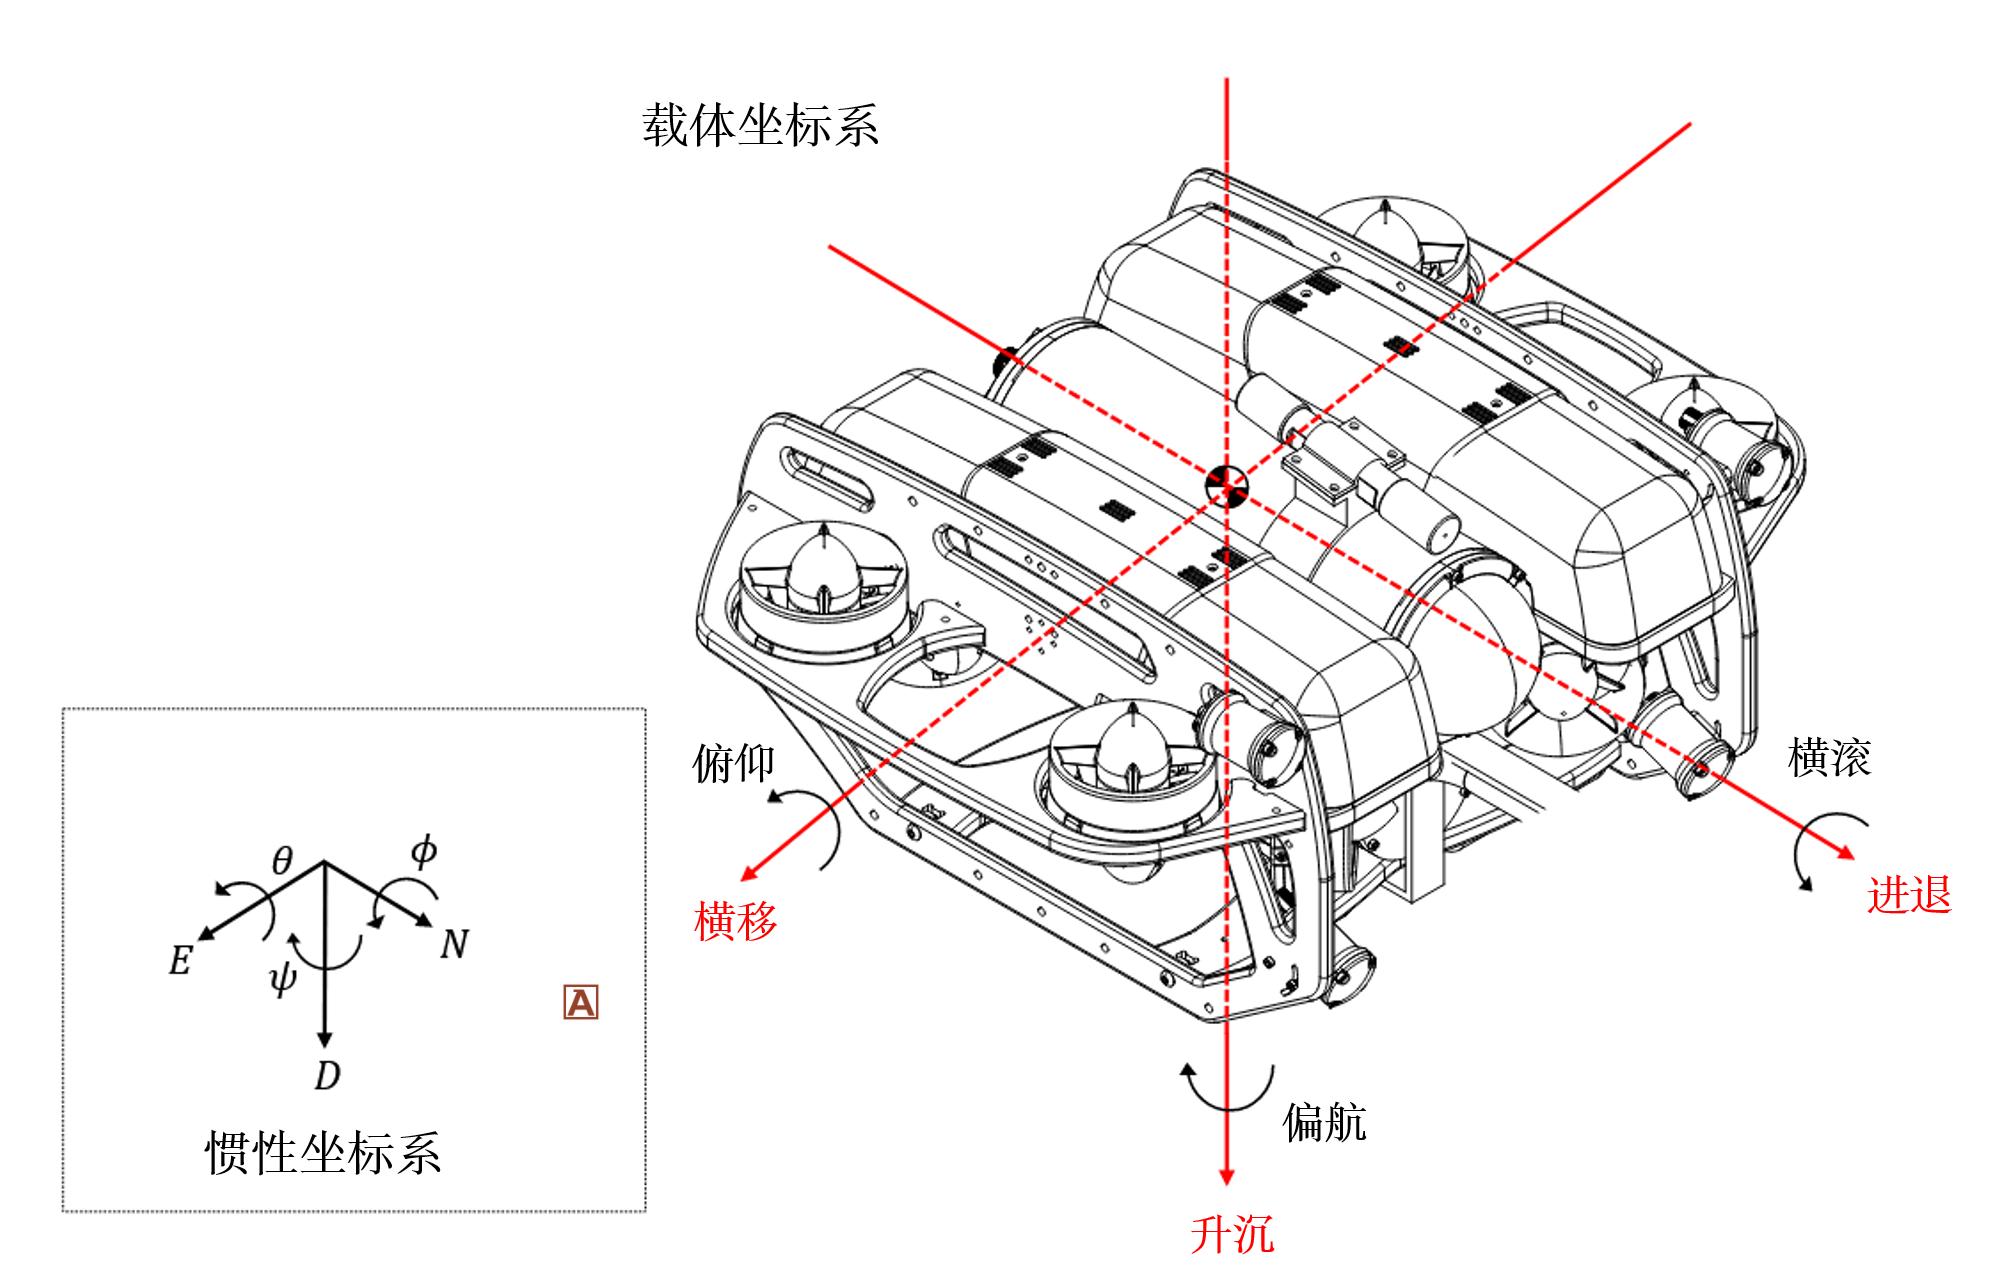
\includegraphics[width=0.8\linewidth]{images/chapter2/frame-identification.png}
    \caption{惯性坐标系与载体坐标系示意图}
    \label{f.frame_identification}
\end{figure}

ROV 的运动位置与姿态一般分别在惯性坐标系和载体坐标系下分别表示。在惯性坐标系下,定义 ROV 的位置向量为$\symbf{\eta}_1 = [x,y,z]^T$,姿态向量为$\symbf{\eta}_2 = [\phi, \theta, \psi]^T$,统称为欧拉角,以$\symbf{\eta} = [\symbf{\eta}_1, \symbf{\eta}_2]=[x,y,z,\phi,\theta,\psi]^T$为惯性坐标系下的广义位姿向量。在载体坐标系下,定义 ROV 沿坐标轴的线速度向量为$\symbf{v}_1 = [u,v,w]^T$,绕坐标轴的角速度向量为$\symbf{v}_2=[p,q,r]^T$,以$\symbf{v} = [\symbf{v}_1,\symbf{v}_2] = [u,v,w,p,q,r]^T$为广义的速度向量。定义 ROV 各方向所受的力沿坐标轴方向的分量组成外力向量$\symbf{\tau}_1=[X, Y, Z]^T$,定义各方向所受力在各坐标轴上产生的力矩为外力矩向量$\symbf{\tau}_2 = [K, M, N]^T$,以$\symbf{\tau}=[\symbf{\tau}_1,\symbf{\tau}_2]=[X, Y, Z ,K, M ,N]^T$为广义受力向量。上述参数的具体定义见表\ref{t.kinetics_params}。

\begin{table}[htb]
  \centering
  \caption{ROV 各坐标系下运动参数定义}
  \zihao{5}
  
  \label{t.kinetics_params}
  \begin{tabular}{cccc}
  \hline
向量 & 惯性坐标系下位姿  & 载体坐标系下速度 & 载体坐标系下受力 \\
\hline
沿$x$轴方向 & $x$  & $u$ & $X$ \\
沿$y$轴方向 & $y$  & $v$ & $Y$ \\
沿$z$轴方向 & $z$  & $w$ & $Z$ \\
绕$x$轴方向 & $\phi$  & $p$ & $K$ \\
绕$y$轴方向 & $\theta$  & $q$ & $M$ \\
绕$z$轴方向 & $\psi$  & $r$ & $N$ \\
\hline
\end{tabular}
\end{table}

\subsection{载体坐标系与惯性坐标系的转换}

在 ROV 的运动控制中,需要对载体坐标系和惯性坐标系下的运动参数进行转换。如 IMU 测得的速度信息往往是在载体坐标系下得到的,而运动控制器所计算的速度信息往往是在惯性坐标系下的速度,因此需要计算两个坐标系之间的转换矩阵,以构建 ROV 的运动学方程。

对于惯性坐标系下的线速度向量$\dot{\symbf{\eta}_1}=[\dot{x},\dot{y},\dot{z}]^T$,角速度向量$\dot{\symbf{\eta}_2} = [\dot{\phi},\dot{\theta},\dot{\psi}]^T$,与惯性坐标系下的线速度向量$\symbf{v}_1=[u,v,w]^T$,角速度向量$\symbf{v}_2=[p,q,r]^T$,他们之间有下列关系:
\begin{equation}
\dot{\symbf{\eta}_1}=\symbf{R}\symbf{v}_1
\label{eq.linear_velocity_trans}
\end{equation}
\begin{equation}
\dot{\symbf{\eta}_2}=\symbf{T}\symbf{v}_2
\label{eq.angular_velocity_trans}
\end{equation}
其中,线速度变换矩阵为:
\begin{equation}
    \symbf{R} = \begin{bmatrix}
        \cos \psi \cos \theta & \sin\psi\sin\theta\sin\phi-\sin\psi\cos\phi & \cos\psi\sin\theta\cos\phi+\sin\psi\sin\phi \\
        \sin\psi\cos\theta & \sin\psi\sin\theta\sin\phi+\cos\psi\cos\phi & \sin\psi\sin\theta\cos\phi-\cos\psi\cos\phi \\
        -\sin\theta & \cos\theta\sin\phi & \cos\theta\cos\phi \\
    \end{bmatrix}
    \label{eq.R_trans}
\end{equation}
对该矩阵求逆,得到:
\begin{equation}
    \symbf{R}^{-1} = \begin{bmatrix}
        \cos\psi\cos\theta & \sin\psi\cos\theta & -\sin\theta \\
        -\sin\psi\cos\theta+\cos\psi\sin\phi\sin\theta & \cos\psi\cos\phi\sin\theta & \cos\theta\sin\phi \\
        -\sin\theta & \cos\theta\sin\phi & \cos\theta\cos\phi \\
    \end{bmatrix}
    \label{eq.R_trans_inv}
\end{equation}
角速度变换矩阵为:
\begin{equation}
    \symbf{T} = \begin{bmatrix}
        1 & \sin\phi\tan\theta & \cos\phi\tan\theta \\
        0 & \cos\phi & -\sin\phi \\
        0 & \sin\phi / \cos\theta & \cos\phi / \cos\theta \\
    \end{bmatrix}
    \label{eq.T_trans}
\end{equation}
对该矩阵求逆,得到:
\begin{equation}
    \symbf{T}^{-1} = \begin{bmatrix}
        1 & 0 & -\sin\theta \\
        0 & \cos\phi & \cos\theta\sin\phi \\
        0 & -\sin\phi & \cos\phi\cos\theta \\
    \end{bmatrix}
    \label{eq.T_trans_inv}
\end{equation}
通过(\ref{eq.linear_velocity_trans}),(\ref{eq.angular_velocity_trans}),(\ref{eq.R_trans}),(\ref{eq.T_trans})联立,可以得到 ROV 运动学方程:
\begin{equation}
    \dot{\symbf{\eta}} = \symbf{J}(\symbf{\eta})\symbf{v}
    \label{eq.kinetics_equation}
\end{equation}
\begin{equation}
    \symbf{J}(\symbf{\eta}) = \begin{bmatrix}
        \symbf{R} & \symbf{0}_{3\times 3} \\
        \symbf{0}_{3\times 3} & \symbf{T} \\
    \end{bmatrix}
    \label{eq.T_trans_inv}
\end{equation}

\section{BlueROV2 动力学模型}

\subsection{电机分布介绍}

BlueROV2 共搭载 6 个 T200 电机,电机分布如图\ref{f.motor_distribution}所示。其中,蓝色推进器为顺时针推进器,绿色推进器为逆时针推进器,红色箭头表示正向前进方向。

\begin{figure}[hbt]
    \centering
    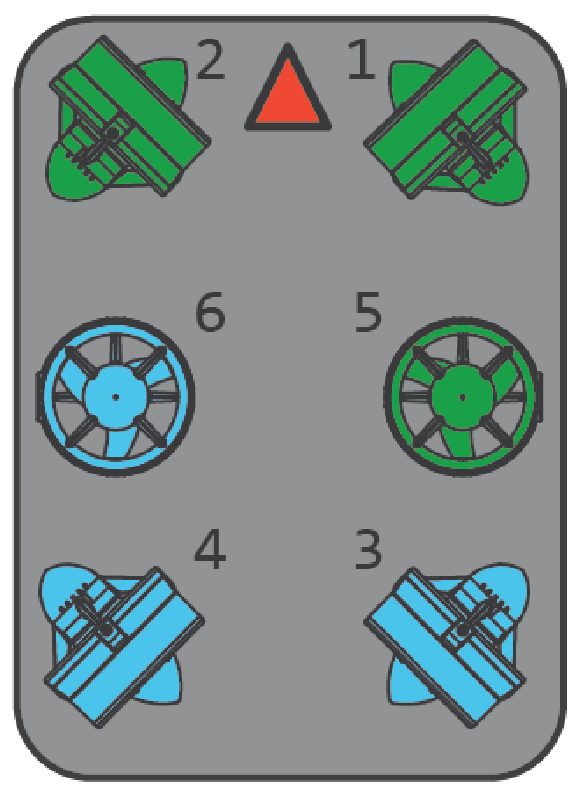
\includegraphics[width=0.2\linewidth]{images/chapter2/motor_distribution.png}
    \caption{BlueROV2 电机分布图}
    \label{f.motor_distribution}
\end{figure}

各电机在载体坐标系下的位置坐标,与电机朝向角度在 BlueROV2 上的设置如表\ref{t.motor_position_rpy}所示。
\begin{table}[htb]
  \centering
  \caption{载体坐标系下的 BlueROV2 电机位置坐标}
  \zihao{5}
  
  \label{t.motor_position_rpy}
  \begin{tabular}{c c c c c c c}
  \hline
电机编号 & X 轴坐标/m  & Y 轴坐标/m & Z 轴坐标/m & 绕 X 旋转/rad & 绕 Y 旋转/rad & 绕 Z 旋转/rad\\
\hline
T1 & 0.1355 & -0.1 & -0.0725 & 0 & 0 & 0.7853 \\
T2 & 0.1355 & 0.1 & -0.0725 & 0 & 0 & -0.7853 \\
T3 & -0.1475 & -0.1 & -0.0725 & 0 & 0 & 2.356\\
T4 & -0.1475 & 0.1 & -0.0725 & 0 & 0 -2.356 & 0\\
T5 & 0.0025 & -0.1105 & -0.005 & 0 & -1.570 & 0\\
T6 & 0.0025 & 0.1105 & -0.005 & 0 & -1.570 & 0\\
\hline
\end{tabular}
\end{table}
BlueROV2 通过 PWM 值控制六个推进器旋转以提供驱动力,通过查询可以得到六个推进器提供推力与 PWM 值呈二次关系,满足:
\begin{equation}
    F = k_1(\text{PWM}-1500)^2 + k_2(\text{PWM}-1500) + k_3
\end{equation}
其中,$F$表示 T200 电机提供推力,$\text{PWM}$表示推进器接收 PWM 值,$k_1,k_2,k_3$表示推力系数。逆时针推进器(正桨)的推力系数满足:
\begin{equation}
    \symbf{k}_\text{正} = [k_1,k_2,k_3]^T = \begin{cases}
  [1.5\times 10^{-6}, 6.0\times 10^{-3} ,7.1\times 10^{-2}], & \text{PWM}>1500 \\
  [0,0,0], & 1460<\text{PWM}<1500, \text{死区} \\
  [-3.3\times 10^{-6}, 6.9\times 10^{-3}, 0.34], & \text{PWM} > 1500 \\
\end{cases}
\end{equation}
顺时针推进器(反桨)的推力系数满足:
\begin{equation}
   \symbf{k}_\text{反} = [k_1,k_2,k_3]^T = \begin{cases}
  [2.5\times 10^{-6}, -5.5\times 10^{-3} ,-0.171], & \text{PWM}>1500 \\
  [0,0,0], & 1470<\text{PWM}<1500, \text{死区} \\
  [-7.9\times 10^{-7}, -7.8\times 10^{-3}, 0.019], & \text{PWM} > 1500 \\
\end{cases}
\end{equation}

\subsection{BlueROV2 受力分析}

在 ROV 的研究与应用中,构建精确的动力学模型是一项具有根本性意义的工作,动力学模型用于描述作用在机器人上的力和力矩与其加速度之间的关系。将 ROV 所受外力进行数学表达是 ROV 动力学建模准确的基础,也是 ROV 运动控制与仿真的前提。

\subsubsection{静力(力矩)}

静力(力矩)是指由于水下航行器自身的重力与所受的浮力共同作用产生的力或力矩。对于 ROV 的重力,一般是将 ROV 的各个部件所受的合力简化到 ROV 主体重心处所受的重力,即重力 $G$ 作用点为重心,类似于重力,ROV 所受的浮力 $B$ 的作用点为浮心。可以得到载体坐标系下的静力方程:
\begin{equation}
    \symbf{g}(\symbf{\eta}) = \begin{bmatrix}
        -(G-B)\sin\theta \\
        (G-B)\cos\theta\sin\phi \\
        (G-B)\cos\theta\cos\phi \\
        -(y_GG-y_BB)\cos\theta\cos\phi + (z_GG-Z_BB)\cos\theta\sin\phi \\
        (z_GG-z_BB)\sin\theta + (x_GG-x_BB)\cos\theta\cos\phi \\
        (x_GG-x_BB)\cos\theta\sin\phi - (y_GG-y_BB)\sin\theta \\
    \end{bmatrix}
    \label{eq.restore_force}
\end{equation}
其中,$x_G,y_G,z_G;x_B,y_B,z_B$分别为 ROV 重心与浮心在载体坐标系下的位置坐标。因为 ROV 载体坐标系原点与重心重合,且 ROV 在浮力配平后,浮心在重心的正上方,所以式(\ref{eq.restore_force})可以简化为
\begin{equation}
    \symbf{g}(\symbf{\eta}) = \begin{bmatrix}
        -(G-B)\sin\theta \\
        (G-B)\cos\theta\sin\phi \\
        (G-B)\cos\theta\cos\phi \\
        -z_BB\cos\theta\sin\phi \\
        -z_BB\sin\theta \\
        0 
    \end{bmatrix}
\end{equation}

\subsubsection{推力器力矩}

图\ref{f.motor_distribution}呈现了 BlueROV2 的推力器分布情况,推进器推力 (力矩) 是指水下机器人安装的螺旋桨或十字舵等推进器提供的驱动力,是 ROV 运动控制策略的执行机构。ROV 的受力向量和推进器提供的推力向量,满足关系
\begin{equation}
     \symbf{\tau} = \symbf{T}\symbf{F}
\end{equation}
其中$\symbf{T}$为推力配置矩阵,满足
\begin{equation}
    \symbf{T} = [\symbf{t}_1, \cdots, \symbf{t}_6]^T
\end{equation}
其中的每个列向量$\symbf{t}_i$将每个推力器产生的力$F_i$与向量$\symbf{\tau}$联系起来:
\begin{equation}
\symbf{t}_i = \begin{bmatrix}
    \symbf{\varepsilon}_i \\
    \symbf{r}_i \times \symbf{\varepsilon}_i
\end{bmatrix}
\end{equation}
其中$\symbf{r}_i$是第$i$个推进器的位置向量,$\symbf{\varepsilon}_i$表示第$i$个推进器的单位推力在三个轴上的分量,定义第$i$个推进器姿态向量为$\symbf{\eta}_{mi}=[\phi_i, \theta_i, \psi_i]^T$,则
\begin{equation}
    \symbf{\varepsilon}_i=[\cos\psi_i\cos\theta_i,\sin\psi_i\cos\theta_i,-\sin\theta_i]
\end{equation}
通过代入各个推进器的姿态向量,可以计算出BlueROV2的推力配置矩阵$\symbf{T}$。
\begin{equation}
    \symbf{T} = \begin{bmatrix}
        0.707 & 0.707 & -0.707 & -0.707 & 0 & 0\\
        -0.707 & 0.707 & -0.707 & 0.707 & 0 & 0 \\
         0 & 0 & 0 & 0 & 1 & 1 \\
         0.051 & -0.051 & 0.051 & -0.051 & 0.111 & -0.111 \\
         0.051 & 0.051 & -0.051 & -0.051 & 0.002 & -0.002 \\
         -0.167 & 0.167 & 0.175 & -0.175 & 0 & 0 \\
    \end{bmatrix}
\end{equation}

\subsubsection{水动力建模}

水动力是指ROV在水下航行过程中周围流体的反作用力,主要包括惯性水动力与粘性水动力。水动力的产生根源在于ROV与周围水体之间的相互作用,影响ROV所受水动力的因素有很多,主要包括ROV的几何外形,航行速度、加速度与流体物理属性的影响。在一般水下作业下,本文假设ROV几何外形基本不变,流体物理属性基本保持一致,以此将ROV的水动力方程简化为ROV速度、加速度的函数。

惯性水动力$F_I(\dot{V})$满足
\begin{equation}
    F_I(\dot{V})=\lambda_{ij}\dot{V}
\end{equation}
其中,$\dot{V}$表示ROV在载体坐标系下的加速度,比例系数$\lambda_{ij}$为附加质量系数。

粘性水动力$F_D(V)$满足
\begin{equation}
    F_D(V) = q_{ij}V
\end{equation}
其中,$V$表示ROV在载体坐标系下的速度,比例系数$q$为一阶阻尼系数。

\subsubsection{其他受力}

ROV在水下航行作业时,其运动状态和控制精度会受到复杂且动态变化的水下环境带来的各种干扰力的影响。这些力来源广泛,既有外部环境因素,也有ROV本体自身特性与环境交互产生的因素。水体环境的复杂多变,会导致动力学模型存在噪音,设由环境产生的非结构性受力为$\symbf{\tau}_e$。

\section{BlueROV2 动力学建模}

鉴于ROV的水下航行可以视为刚体六自由度运动,使用刚体牛顿-欧拉运动方程对ROV进行运动学建模,动力学方程如下:
\begin{equation}
    \symbf{M}\dot{\symbf{V}}+\symbf{C}(\symbf{v})+\symbf{D}(\symbf{v})+\symbf{g}(\symbf{\eta}) = \symbf{\tau} + \symbf{\tau}_e
\end{equation}
其中,$\symbf{M} = \symbf{M}_{RB}+\symbf{M}_a$,分别为ROV的刚体质量矩阵和附加质量矩阵;$\symbf{C}(\symbf{v})=\symbf{C}_{RB}(\symbf{v})+\symbf{C}_a(\symbf{v})$,分别为ROV的刚体科里奥利力矩阵和附加科里奥利力矩阵;$\symbf{D}(\symbf{v})=\symbf{D}_l(\symbf{v})+\symbf{D}_q(\symbf{v})$,分别为ROV所受的一阶流体阻力和二阶流体阻力;$\symbf{g}(\symbf{\eta})$为ROV所受重力与浮力共同组成的恢复力,即上文所提到的静力(力矩);$\symbf{\tau}$为6个电机提供的驱动力与驱动力矩;$\symbf{\tau}_e$为ROV在水下航行过程中由于环境等不可控因素导致的受力。

上述动力学方程中,ROV的质量矩阵满足$\symbf{M}_{RB}=\symbf{M}_{RB}^T>0$,满足
\begin{equation}
    \symbf{M}_{RB}=\begin{bmatrix}
        m\symbf{I}_{3\times 3} & -mS(r_g^b) \\
        mS(r_g^b) & \symbf{I}_b \\
    \end{bmatrix} = \begin{bmatrix}
        m & 0 & 0 & 0 & mz_g & -my_g \\
        0 & m & 0 & -mz_g & 0 & mx_g \\
        0 & 0 & m & my_g & -mx_g & 0 \\
        0 & -mz_g & my_g & I_x & -I_{xy} & -I_{xz} \\
        mz_g & 0 & -mx_g & -I_{yx} & I_y & -I_{yz} \\
        -my_g & mx_g & 0 & -I_{zx} & -I_{zy} & I_z \\
    \end{bmatrix}
\end{equation}
其中,$m$为ROV质量,$r_g^b = [x_g,y_g,z_g]^T$为载体坐标系下的质心的位置坐标,由于载体坐标系下原点与ROV的质心重合,故$r_g^b=[0,0,0]^T$;上式中
 $$I_x = \int_V(y^2+z^2)\rho_mdV$$
 $$I_y = \int_V(x^2+z^2)\rho_mdV$$
 $$I_z = \int_V(x^2+y^2)\rho_mdV$$
 $$I_xy = \int_Vxy\rho_mdV=I_{yx}$$
 $$I_xz = \int_Vxz\rho_mdV=I_{zx}$$
\begin{equation}
 I_yz = \int_Vyz\rho_mdV=I_{zy}
\end{equation}
设三条坐标轴为中心惯性主轴,则$I_{xy} = I_{yz} = I_{xz} = 0$,$\symbf{I_b} = diag([I_x, I_y, I_z])$;$S(\cdot)$为矢量相乘算子,满足:
$$\symbf{\lambda}\times \symbf{a}:=\symbf{S}(\symbf{\lambda})\symbf{a}$$
\begin{equation}
    \symbf{S}(\symbf{\lambda})=-\symbf{S}^T(\symbf{\lambda})=\left[
    \begin{matrix}
    0 & -\lambda_3 & \lambda_2 \\
    \lambda_3 & 0 & -\lambda_1 \\
    -\lambda_2 & \lambda_1 & 0 \\
    \end{matrix}
    \right], \symbf{\lambda}=\left[
    \begin{matrix}
    \lambda_1 \\
    \lambda_2 \\
    \lambda_3 \\
    \end{matrix}
    \right]
\end{equation}
由此可以得到刚体质量矩阵的表达式
\begin{equation}
    \symbf{M}_{RB} = \begin{bmatrix}
        m\symbf{I}_{3\times 3} & -mS(r_g^b) \\
        mS(r_g^b) & \symbf{I}_b \\
    \end{bmatrix} = \begin{bmatrix}
    m & 0 & 0 & 0 & 0 & 0 \\
    0 & m & 0 & 0 & 0 & 0 \\
    0 & 0 & m & 0 & 0 & 0 \\
    0 & 0 & 0 & I_x & 0 & 0 \\
    0 & 0 & 0 & 0 & I_y & 0 \\
    0 & 0 & 0 & 0 & 0 & I_z \\
\end{bmatrix}
\end{equation}
附加质量矩阵满足
\begin{equation}
    \symbf{M}_a = diag([X_{\dot{u}},Y_{\dot{v}},Z_{\dot{w}},K_{\dot{p}},M_{\dot{q}},N_{\dot{r}}])
\end{equation}
其中,$X_{\dot{u}},Y_{\dot{v}},Z_{\dot{w}},K_{\dot{p}},M_{\dot{q}},N_{\dot{r}}$为ROV附加质量系数。

对质量矩阵进行处理
\begin{equation}
\symbf{M} = \begin{bmatrix}
    \symbf{M}_{11} & \symbf{M}_{12} \\
    \symbf{M}_{21} & \symbf{M}_{22} \\
\end{bmatrix}    
\end{equation}
可以得到科里奥利力矩阵$\symbf{C}(\symbf{v})$为:
\begin{equation}
    \symbf{C}(\symbf{v}) = \begin{bmatrix}
        \symbf{0}_{3\times 3} & -S(\symbf{M}_{11}\symbf{v}_1+\symbf{M}_{12}\symbf{v}_2) \\ 
        -S(\symbf{M}_{11}\symbf{v}_1+\symbf{M}_{12}\symbf{v}_2) & -S(\symbf{M}_{21}\symbf{v}_1+\symbf{M}_{22}\symbf{v}_2)
    \end{bmatrix}
\end{equation}
其中,$\symbf{v}_1 = [u,v,w]^T,\symbf{v}_2=[p,q,r]^T$,由此可以得到科里奥利力矩阵的表达式
\begin{equation}
    \symbf{C}_{RB}(\symbf{v})=
\begin{bmatrix}
    0 & 0 & 0 & 0 & mw & -mv \\
    0 & 0 & 0 & -mw & 0 & mu \\
    0 & 0 & 0 & mv & -mu & 0 \\
    0 & mw & -mv & 0 & I_zr & -I_yq \\
    -mw & 0 & mu & -I_zr & 0 & I_xp \\
    mv & -mu & 0 & I_yq & -I_xp & 0 \\
\end{bmatrix}
\end{equation}

\begin{equation}
    \symbf{C}_a(\symbf{v})=
\begin{bmatrix}
    0 & 0 & 0 & 0 & -Z_{\dot{w}}w & Y_{\dot{v}}v \\
    0 & 0 & 0 & Z_{\dot{w}}w & 0 & -X_{\dot{u}}u \\
    0 & 0 & 0 & -Y_{\dot{v}}v & X_{\dot{u}}u & 0 \\
    0 & -Z_{\dot{w}}w & Y_{\dot{v}}v & 0 & -N_{\dot{r}}r & M_{\dot{q}}q \\
    Z_{\dot{w}}w & 0 & -X_{\dot{u}}u & N_{\dot{r}}r & 0 & -K_{\dot{p}}p \\
    -Y_{\dot{v}}v & X_{\dot{u}}u & 0 & -M_{\dot{q}}q & K_{\dot{p}}p & 0 \\
\end{bmatrix}
\end{equation}
ROV所受的一阶水动力阻尼和二阶水动力阻尼可分别用(\ref{eq.linear_damping}),(\ref{eq.square_damping})表示
\begin{equation}
    \symbf{D}_l=-diag([X_u,Y_v,Z_w,K_p,M_q,N_r])
    \label{eq.linear_damping}
\end{equation}
\begin{equation}
    \symbf{D}_{q}(\symbf{v}) = -diag([X_{u|u|}|u|,Y_{v|v|}|v|,Z_{w|w|}|w|,K_{p|p|}|p|,M_{q|q|}|q|,N_{r|r|}|r|])
    \label{eq.square_damping}
\end{equation}
其中,$X_u,Y_v,Z_w,K_p,M_q,N_r$为一阶水阻尼系数,$X_{u|u|},Y_{v|v|},Z_{w|w|},K_{p|p|},M_{q|q|},N_{r|r|}$为二阶水阻尼系数。

至此,本文获得简化后的BlueROV2动力学方程,方程中相关物理信息可以通过实际测量得到,见表\ref{t.physical_params}所示。

\begin{table}[htb]
  \centering
  \caption{BlueROV2物理参数表}
  \zihao{-5}
  \label{t.physical_params}
  \begin{tabular}{c c c c c c c c}
  \hline
参数名 & 质量($m$) & 惯性矩($I_x$)& 惯性矩($I_y$) & 惯性矩($I_z$) & 重力($G$) & 浮力($B$) & 浮心$z$轴坐标  \\
\hline
参数值 & 11.2 & 0.303 & 0.626 & 0.576 & 112.80 & 111.47 & 0.02 \\
单位 & $kg$ & $kg\cdot m^2$ & $kg\cdot m^2$ & $kg\cdot m^2$ &  N & N & m \\
\hline
\end{tabular}
\end{table}

\subsection{本章小结}

本章围绕BlueROV2的运动学与动力学建模展开了详细的论述。首先介绍了ROV的结构设计特点,为后续的建模分析奠定了基础。在运动学建模部分,重点明确了坐标系的建立规则和运动参数的定义,并详细推导了载体坐标系与惯性坐标系之间的转换关系,用于描述ROV空间位姿与运动参数的关系。随后,章节深入到BlueROV2的动力学模型构建,首先概述了其电机的分布情况,接着对BlueROV2进行了全面的受力分析,具体探讨了作用在ROV上的静力、推进器产生的推力与力矩、复杂的水动力以及其他可能的环境扰动力。在分别对各项力进行建模和分析的基础上,最终整合形成了BlueROV2的完整动力学方程,为后续的仿真分析、控制器设计以及运动特性研究提供了数学依据和理论支持。

\newpage

%%%%%%%%%%%%%%%%%%%%%%%%%%%%%%%%图像插入示例%%%%%%%%%%%%%%%%


%%%%%%%%%%%%%%%%%%%%%%%%%%%%%%%%表格插入示例%%%%%%%%%%%%%%%%
%!TEX root = ../../csuthesis_main.tex
\chapter{ROV动力学模型参数辨识}
\section{ROV水动力系数辨识方法}

\subsection{最小二乘辨识ROV水动力系数}
最小二乘算法是最早提出的参数估计算法,旨在找到一组未知参数,使得模型输出尽可能贴近实际观测数据。本节利用最小二乘法进行ROV水平面动力学方程的水动力系数辨识,之后将辨识的结果作为RNN深度学习网络参数辨识的参考值。

首先简要介绍最小二乘法。假设未知参数为$X$,状态维度为$n$,一般的传感器或观测手段无法直接测量$X$的具体数值,只能观测$X$各分量的线性组合,假设第$i$个时间步上,$X$满足方程:\begin{equation}
    Z_i=\mathbf{H_i}X+V_i
\end{equation}
式中$Z_i$为$m_i$维向量,$\mathbf{H_i}$和$V_i$分别为第$i$个时间步观测的状态矩阵和测量噪声,假设共进行$r$次观测采样,则有:
\begin{equation}
\left\{\begin{matrix}
Z_1 = \mathbf{H_i}X+V_1\\
Z_2 = \mathbf{H_i}X+V_2\\
\vdots \\
Z_r = \mathbf{H_i}X+V_r\\
\end{matrix}\right. 
\end{equation}

最小二乘算法的核心是使由未知参数的估计值$\hat{X}$计算出的预测值$\hat{Z_i}=\mathbf{H_i}\hat{X}+V_i$和观测值$Z_i$之间的误差平方和最小,定义损失函数为:
\begin{equation}
    J(\hat{X})=\sum_{i=1}^r(Z_i-\mathbf{H_i}\hat{X})^2
\end{equation}
对上述过程中的$\hat{X}$求偏导,当导数为$0$时$J$存在最小值:
\begin{equation}
    \left.\frac{\partial J}{\partial \hat{X}}\right|_{X=\hat{X}}=-2 \mathbf{H}^{T}(Z-\mathbf{H} \hat{X})=0
\end{equation}
则最小二乘法的估计值为:
\begin{equation}
    \hat{X}=(\mathbf{H}^T\mathbf{H})^{-1}\mathbf{H}^TZ
\end{equation}
本节在开始最小二乘辨识之前,先利用高保真仿真平台Gazebo产生Bluerov2在静水中的航行仿真数据,采样频率为$20Hz$,记录电机转速、在全局坐标系下的位置和姿态序列、线速度和角速度序列、线加速度和角加速度序列。在后续辨识过程中,为了模拟实际航行数据,对仿真中的速度序列添加噪声来模拟传感器的采样值,假设速度噪声概率统计满足高斯分布,则采用如下方式添加噪声:
\begin{equation}
\begin{bmatrix}
u_t^*\\
v_t^*\\
w_t^*\\
\end{bmatrix} = \begin{bmatrix}
u_t\\
v_t\\
w_t\\
\end{bmatrix} + randn(0,0.01)
\end{equation}

式中$[u_t^*,v_t^*,w_t^*]^T$表示带有噪声速度数据,$[u_t,v_t,w_t]^T$表示仿真采样速度数据,其中,$randn(0,0.01)\in \mathbb{R}^{3x1}$表示满足均值为0,方差为0.01高斯分布的噪声数据。定义仿真中的真实ROV水动力系数如表\ref{t.real_hydro_coff}所示,ROV基本参数如表\ref{t.rov_base_params}所示。
\begin{table}[htb]
  \centering
  \caption{仿真平台中ROV真实水动力系数}
  \label{t.real_hydro_coff}
  \begin{tabular}{ccccccc}
  \hline
符号 & $X_{\dot{u}}$ & $Y_{\dot{v}}$ & $Z_{\dot{w}}$ & $K_{\dot{p}}$ & $M_{\dot{q}}$ & $N_{\dot{r}}$ \\
\hline
值  & -1.7182         & 0         & -5.468        & 0         & -1.2481         & -0.4006         \\
\hline
\hline
符号 & $X_u$         & $Y_v$         & $Z_w$         & $K_p$         & $M_q$         & $N_r$         \\
\hline
值  & -11.7391         & -20         & -31.8678         & -25         & -44.9085         & -5         \\
\hline
\hline
符号 & $X_{u|u|}$    & $Y_{v|v|}$    & $Z_{w|w|}$    & $K_{p|p|}$    & $M_{q|q|}$    & $N_{r|r|}$    \\
\hline
值  & 0        & 0        & 0        & 0         & 0         & 0 \\  
\hline
\end{tabular}
\end{table}

\begin{table}[htb]
  \centering
  \caption{仿真平台中ROV基本参数}
  \label{t.rov_base_params}
\begin{tabular}{cccccccc}
\hline
符号 & $m$  & $I_x$ & $I_y$ & $I_z$ & $(x_g,y_g,z_g)$ & $\rho_{water}$ & $V$   \\
\hline
值  & 11.2$kg$ & 0.16$kg m^2$  & 0.16$kg m^2$  & 0.16$kg m^2$  & (0,0,0.02$m$)      & 1.028$kg/m^3$        & 11.31$m^3$  \\
\hline
\end{tabular}
\end{table}

\subsection{水平面运动上的最小二乘辨识}
根据上述最小二乘辨识方法,本节首先对运动方程进行解耦,利用ROV水平运动轨迹估计水平面运动中的水动力系数。水平面运动是速度向量被约束到某水平面内和角速度向量保持与水平面垂直的运动形式。在机体坐标系下,由于ROV速度向量$U$始终保持在$oxy$平面内,故冲角$\alpha = 0$,漂角$\beta \ne 0$,又有角速度向量保持与水平面垂直,故线速度中$w=\dot{w}=0$,$p=q=\dot{p}=\dot{q}=0$,将该条件代入动力学分量方程,可以得到ROV在水平面上运动方程各分量的简化形式:


\begin{equation}
\begin{aligned}
X & =(m-X_{\dot{u}})\dot{u}+ (Y_{\dot{v}}-m)vr+(-X_u-X_{u|u|}|u|)u \\
Y & =(m-Y_{\dot{v}})\dot{v}+(m-X_{\dot{u}})ur+(-Y_v-Y_{v|v|}|v|)v \\
N & =(I_z-N_{\dot{r}})\dot{r}+(X_{\dot{u}}-Y_{\dot{v}})vu+(-N_r-N_{r})r 
\end{aligned}
\end{equation}
对前向方程进行整理,可以得到:
\begin{equation}
    \dot{u}=a_1vr+a_2u+a_3u|u|+a_4X
\end{equation}
其中,
\begin{equation}
    a_1=\frac{m-Y_{\dot{v}}}{m-X_{\dot{u}}},a_2=\frac{X_u}{m-X_{\dot{u}}},a_3=\frac{X_{u|u|}}{m-X_{\dot{u}}},a_4=\frac{1}{m-X_{\dot{u}}}
\end{equation}
这四个数为最小二乘法代求系数,按照上述最小二乘算法进行整理,可以得到:
\begin{equation}
    \begin{bmatrix}
    \dot{u}_1 \\
    \dot{u}_2 \\
    \vdots \\
    \dot{u}_T \\
    \end{bmatrix}
    =
    \begin{bmatrix}
    v_1r_1 & u_1 & u_1|u_1| & X_1 \\
    v_2r_2 & u_2 & u_2|u_2| & X_2 \\
    \vdots & \vdots & \vdots & \vdots \\
    v_Tr_T & u_T & u_T|u_T| & X_T \\
    \end{bmatrix}
    \begin{bmatrix}
    a_1 \\
    a_2 \\
    \vdots \\
    a_T \\
    \end{bmatrix}
\end{equation}
式中,$[a_1,a_2,a_3,a_4]^T$为待估计参数,根据上式可以求解出这4个变量,之后先求解$a_4$中的$X_{\dot{u}}$后,可以依次求解出$a_1,a_2,a_3$中的$Y_{\dot{v}},X_u,X_{u|u| }$变量。按照这个方法,ROV侧向运动的动力学方程可整理为:
\begin{equation}
    \dot{v}=b_1ur+b_2v+b_3v|v|+b_4Y
\end{equation}
其中,
\begin{equation}
    b_1=\frac{X_{\dot{u}}-m}{m-Y_{\dot{v}}},b_2=\frac{Y_v}{m-Y_{\dot{v}}},b_3=\frac{Y_{v|v|}}{m-Y_{\dot{v}}},b_4=\frac{1}{m-Y_{\dot{v}}}
\end{equation}

这四个数为最小二乘法代求系数,按照上述最小二乘算法进行处理,可以得到:
\begin{equation}
    \begin{bmatrix}
    \dot{v}_1 \\
    \dot{v}_2 \\
    \vdots \\
    \dot{v}_T \\
    \end{bmatrix}
    =
    \begin{bmatrix}
    u_1r_1 & v_1 & v_1|v_1| & Y_1 \\
    u_2r_2 & v_2 & v_2|v_2| & Y_2 \\
    \vdots & \vdots & \vdots & \vdots \\
    u_Tr_T & v_T & v_T|v_T| & Y_T \\
    \end{bmatrix}
    \begin{bmatrix}
    b_1 \\
    b_2 \\
    \vdots \\
    b_T \\
    \end{bmatrix}
\end{equation}
式中,$[b_1,b_2,b_3,b_4]^T$为待估计参数,根据上式可以求解出这4个变量,之后先求解$b_4$中的$Y_{\dot{v}}$后,可以依次求解出$b_1,b_2,b_3$中的$X_{\dot{u}},Y_v,Y_{v|v| }$变量。

但是考虑到在这两个式子中,$X_{\dot{u}}$与$Y_{\dot{v}}$均得到了两次估计值,为了减小误差,采用两次估计值的平均值作为$X_{\dot{u}}$和$Y_{\dot{v}}$的最终估计值:
\begin{equation}
    \begin{aligned}
        X_{\dot{u}} & =m + \frac{1}{2}\left(\frac{b_1}{b_4}-\frac{1}{a_4}\right)\\
        Y_{\dot{v}}& =m + \frac{1}{2}\left(\frac{a_1}{a_4}-\frac{1}{b_4}\right)
    \end{aligned}
\end{equation}


类似地,可以将ROV水平面回转运动方程整理为:
\begin{equation}
    \dot{r}=c_1vu+c_2r+c_3r|r|+c_4N
\end{equation}

其中,
\begin{equation}
    c_1=\frac{Y_{\dot{v}}-X_{\dot{u}}}{I_z-N_{\dot{r}}},c_2=\frac{N_r}{I_z-N_{\dot{r}}}, c_3=\frac{N_{r|r|}}{I_z-N_{\dot{r}}},c_4=\frac{1}{I_z-N_{\dot{r}}}
\end{equation}
这四个数为最小二乘法代求系数,按照上述最小二乘算法进行处理,可以得到:
\begin{equation}
    \begin{bmatrix}
    \dot{r}_1 \\
    \dot{r}_2 \\
    \vdots \\
    \dot{r}_T \\
    \end{bmatrix}
    =
    \begin{bmatrix}
    v_1u_1 & r_1 & r_1|r_1| & N_1 \\
    v_2u_2 & r_2 & r_2|r_2| & N_2 \\
    \vdots & \vdots & \vdots & \vdots \\
    v_Tu_T & r_T & r_T|r_T| & N_T \\
    \end{bmatrix}
    \begin{bmatrix}
    c_1 \\
    c_2 \\
    \vdots \\
    c_T \\
    \end{bmatrix}
\end{equation}
式中,$[c_1,c_2,c_3,c_4]^T$为待估计参数,根据上式可以求解出这4个变量,其中$c_1$中的$X_{\dot{u}}$和$Y_{\dot{v}}$代入上述由两次取平均得到的最终估计值,并且将$c_1$与$c_4$计算得到的两个$N_{\dot{r}}$估计值的平均值作为$N_{\dot{r}}$的最终估计值,之后可以依次求解出$c_2,c_3$中的$N_r,N_{r|r|}$变量。$N_{\dot{r}}$的最终估计值为:
\begin{equation}
    N_{\dot{r}} = I_z - \frac{1}{2}(\frac{1}{c_4} + \frac{Y_{\dot{v}}-X_{\dot{u}}}{c_1})
\end{equation}

水平面运动的最小二乘辨识结果如表\ref{t._hydro_coff_ident_horizon}所示。

\begin{table}[htb]
  \centering
  \caption{ROV水平面运动水动力系数辨识结果}
  \label{t._hydro_coff_ident_horizon}
  \begin{tabular}{ccccccc}
  \hline
符号 & $X_{\dot{u}}$ & $Y_{\dot{v}}$ & $N_{\dot{r}}$ \\
\hline
辨识值  & -1.98          & -0.2410          & -0.6560         \\
\hline
\hline
符号 & $X_u$         & $Y_v$            & $N_r$         \\
\hline
辨识值  & -9.3790         & -4.180            & -18.780         \\
\hline
\hline
符号 & $X_{u|u|}$    & $Y_{v|v|}$     & $N_{r|r|}$    \\
\hline
辨识值  & -0.78        & -4.77            & -1.73 \\  
\hline
\end{tabular}
\end{table}

通过辨识出的水动力系数计算动力学模型的前向推导,结果如图\ref{f.dynamic_forward_identified}所示。该曲线图将预测数据与高保真仿真平台下的仿真数据进行对比,两支曲线均是对于相同水下机器人,在相同水环境和相同推进器驱动力下运行,通过计算误差可以发现,$u,v,r$误差范围保持在真值的$1\%$之内,并且辨识得到的运动数据误差累计效应表现不显著,能够有效还原BlueROV2的运动数据。
\begin{figure}[hbt]
    \centering
    \includegraphics[width=\linewidth]{images/chapter3/3.1 水平面最小二乘辨识.jpg}
    \caption{采用水动力系数估计值的水平面前向动力学推导}
    \label{f.dynamic_forward_identified}
\end{figure}
\subsection{竖直面运动的最小二乘辨识}

通过上述方法,本文在高保真仿真平台内使用控制器控制BlueROV2产生一组竖直面内的运动,竖直面运动是速度向量被约束到竖直面内和角速度向量保持与竖直面垂直的运动形式,在机体坐标系下,满足$v=u=\dot{v}=\dot{u}=0$,$r=\dot{r}=0$,将该条件代入动力学分量方程后依照上述方法转换成最小二乘形式,可以辨识出ROV系统水动力系数如表\ref{t._hydro_coff_ident_vertical}所示。

通过辨识出的水动力系数计算动力学模型的前向推导,结果如图\ref{f.dynamic_forward_identified_vertical}所示。将预测数据与高保真仿真平台下的仿真数据进行对比,两支曲线均是对于相同水下机器人,在相同水环境和相同推进器驱动力下运行,通过计算误差可以发现,$w,p,q$误差波动较大,表现不如水平面运动下的最小二乘辨识,但是也能较好拟合实际轨迹运动数据。

\begin{table}[htb]
  \centering
  \caption{ROV竖直面运动水动力系数辨识结果}
  \label{t._hydro_coff_ident_vertical}
  \begin{tabular}{ccccccc}
  \hline
符号 & $Z_{\dot{w}}$ & $K_{\dot{p}}$ & $M_{\dot{q}}$ \\
\hline
辨识值  & -14.57   & -0.12  &   -3.45         \\
\hline
\hline
符号 & $Z_w$         & $K_p$            & $M_q$         \\
\hline
辨识值  & -25.89         & -30.40       & -45.90         \\
\hline
\hline
符号 & $Z_{w|w|}$    & $K_{p|p|}$     & $M_{q|q|}$    \\
\hline
辨识值  & -3.21        & -5.21        & -0.23 \\  
\hline
\end{tabular}
\end{table}

\begin{figure}[hbt]
    \centering
    \includegraphics[width=\linewidth]{images/chapter3/竖直面最小二乘辨识.png}
    \caption{采用水动力系数估计值的竖直面前向动力学推导}
    \label{f.dynamic_forward_identified_vertical}
\end{figure}

\subsection{六自由度运动的最小二乘辨识}
本节对六个自由度的机器人运动过程,采用最小二乘方法辨识水动力系数。对于完整的动力学分量形式,可以将其整理为最小二乘法的形式。

定义在第$i$个时间步下,有矩阵:
\begin{equation}
    F_i
    =\left[
    \begin{matrix}
        X_i-m\dot{u}_i-(w_iq_i-v_ir_i)m\\
        Y_i-m\dot{v}_i-(u_ir_i-w_ip_i)m\\
        Z_i-m\dot{w}_i-(v_ip_i-u_iq_i)m\\
        K_i-I_x\dot{p}_i-q_ir_i(J_z-J_y)\\
        M_i-I_y\dot{q}_i-r_ip_i(J_x-J_z)\\
        N_i-I_z\dot{r}_i-p_iq_i(J_y-J_x)\\
    \end{matrix}
\right]
\end{equation}


\begin{equation}
    \mathbf{A_1} = 
    \left[
    \small
    \begin{matrix}
        -\dot{u}_i & v_ir_i & -w_iq_i & 0 & 0 & 0 \\
        -u_ir_i & -\dot{v}_i & w_ip_i & 0 & 0 & 0 \\
        u_iq_i & -v_ip_i & -\dot{w}_i & 0 & 0 & 0 \\
        0 & v_iw_i & -v_iw_i & -\dot{p}_i & q_ir_i & -q_ir_i \\
        -u_iw_i & 0 & u_iw_i & -r_ip_i & -\dot{q}_i & r_ip_i \\
        u_iv_i & -u_iv_i & 0 & p_iq_i & -p_iq_i & -\dot{r}_i \\
    \end{matrix}
    \right]
\end{equation}
\begin{equation}
    \mathbf{A_2} = -diag([u_i,v_i,w_i,p_i,q_i,r_i])
\end{equation}
\begin{equation}
    \mathbf{A_3} = -diag([u_i|u_i|,v_i|v_i|,w_i|w_i|,p_i|p_i|,q_i|q_i|,r_i|r_i|]) 
\end{equation}
\begin{equation}
    \mathbf{A}=[\mathbf{A_1}, \mathbf{A_2}, \mathbf{A_3}] 
\end{equation}
\begin{equation}
    \Theta_1 = [X_{\dot{u}}, Y_{\dot{v}}, Z_{\dot{w}}, K_{\dot{p}}, M_{\dot{u}}, N_{\dot{r}}]^T
\end{equation}
\begin{equation}
    \Theta_2 = [X_u, Y_v, Z_w, K_p, M_q, N_r]
\end{equation}
\begin{equation}
    \Theta_3 = [X_{u|u|}, Y_{v|v|}, Z_{w|w|}, K_{p|p|}, M_{q|q|}, N_{r|r|}]
\end{equation}
\begin{equation}
    \Theta = [ \Theta_1, \Theta_2, \Theta_3 ]
\end{equation}
\begin{equation}
    \boldsymbol{F} = \boldsymbol{A}\boldsymbol{\Theta}
\end{equation}

通过该组实验,发现直接对六自由度运动过程进行辨识,会导致ROV动力学方程的前向推导发散,经过模型对比分析,动力学模型的发散应该是由于六自由度联动辨识导致不适定或误差放大。最小二乘法要求回归矩阵 $A$ 的列向量彼此线性独立,才能稳定解出参数,但实际运行过程中可能各个自由度之间存在强耦合关系,某些列之间高度相关,使得最小二乘结果不稳定且导致模型发散。

\section{扩展卡尔曼滤波器辨识水动力系数}

接下来,本研究采用扩展卡尔曼滤波器(EKF)从六自由度运动过程辨识水动力系数, EKF辨识算法是在经典线性卡尔曼滤波方法的基础上发展而来的,其显著的优势在于基于状态空间局部线性化点(Kalman滤波值)和测量局部线性化点附近的泰勒级数展开对ROV非线性动力学系统模型进行局部线性化,适用于动态非线性模型。

一般地,离散水动力辨识方法可视为有限输入的灰箱结构,该结构迭代地对ROV动力学模型进行参数估计。由于待定系数的状态空间维数与输入输出的状态空间维数之间不相容,18个水动力线性阻尼系数将无法直接辨识,需要将其作为额外的状态变量$\Theta $增广到EKF算法的状态空间转换模型中。

\subsection{扩展卡尔曼滤波器算法简介}

为引入扩展卡尔曼滤波器,首先定义增广状态向量$\hat{X}_{k-1|k-1}$,满足
\begin{equation}
    \hat{X}_{k-1|k-1} = [u,v,w,p,q,r,\phi, \theta, \psi, \Theta]^T_{k-1|k-1}  
\end{equation}
定义由传感器测量得到的测量向量$Z_k$,满足
\begin{equation}
    Z_k=[u,v,w,p,q,r,\phi,\theta,\psi]^T
\end{equation}
由此,系统状态转移方程可以被定义为:
\begin{equation}
    X_k=f_a\left(\hat{X}_{k-1|k-1}, \Theta_{k-1}, u_{k-1}, k-1\right) + \Phi_{k|k-1}\left(X_{k-1}-\hat{X}_{k-1|k-1}\right) + \gamma_{k|k-1}W_{k-1}
\end{equation}

系统测量方程被定义为:
\begin{equation}
    Z_k = h\left(\hat{X}_{k|k-1},k\right)+H_k\left(X_k-\hat{X}_{k|k-1}\right)+M_kV_k
\end{equation}

其中,

$f_a(\cdot)$为增广动力学模型方程;

$h(\cdot)$为系统测量方程;

$\Phi_{k|k-1}=\{\partial f_a(\hat{X}_{k-1|k-1}, \Theta_{k-1}, u_{k-1}, k-1)/\partial X \}|_{\hat{X}_{k-1|k-1}}$为第$k$时间步下的先验增广状态空间转移雅各比矩阵;

$\gamma_{k|k-1}=\{\partial f_a(\hat{X}_{k-1|k-1}, \Theta_{k-1}, u_{k-1}, k-1)/\partial W\}|_{\hat{X}_{k-1|k-1}}$为第$k$时间步下的先验系统过程噪声雅各比矩阵;

$H_k=\{\partial h(\hat{X}_{k|k-1},k)/\partial X\}|_{\hat{X}_{k-1|k-1}}$为第$k$时间步下的系统测量雅各比矩阵;

$M_k=\{\partial h(\hat{X}_{k|k-1},k)/\partial V\}|_{\hat{X}_{k-1|k-1}}$为第$k$时间步下的系统测量噪声雅各比矩阵。

这样,类似于线性卡尔曼滤波方法,ROV的扩展准线性系统模型可以通过离散EKF算法依次经过时间更新阶段和测量更新阶段从式中辨识出来。时间更新阶段满足:

\begin{equation}
    \begin{aligned}
            \hat{X}_{k|k-1} & =f_a\left(\hat{X}_{k-1|k-1}, \Theta_{k-1}, u_{k-1}, k-1\right) \\
            \mathbf{P}_{k|k-1} & = E\left[\tilde{X}_{k|k-1},\tilde{X}^T_{k|k-1} \right] \\ 
              & =E\left[(\Phi_{k|k-1}\tilde{X}_{k-1|k-1} + \gamma_{k|k-1}W_{k-1})(\Phi_{k|k-1}\tilde{X}_{k-1|k-1} + \gamma_{k|k-1}W_{k-1})^T\right] \\
              & =\Phi_{k|k-1}\mathbf{P}_{k-1|k-1}\Phi_{k|k-1}^T + \gamma_{k|k-1}Q_{k-1}\gamma_{k|k-1}^T
    \end{aligned}
\end{equation}

测量更新阶段满足:
\begin{equation}
\begin{aligned}
        \varepsilon_{k} & =Z_k - H_k\hat{X}_{k|k-1} \\
                        & = H_k\tilde{X}_{k|k-1} + M_kV_k \\
        E\left[\varepsilon_k, \varepsilon_k^T\right] & = H_kP_{k|k-1}H_k^T + M_kR_kM_k^T \\
        K_k  & = E\left[X_k, \varepsilon_k^T\right]E\left[\varepsilon_k, \varepsilon_k^T\right]^{-1} \\
        & =E\left[\left(\hat{X}_{k|k-1}+\tilde{X}_{k|k-1}\right)\left(H_k\tilde{X}_{k|k-1} + M_kV_k\right)^T\right](H_kP_{k|k-1}H_k^T + M_kR_kM_k^T)^{-1}\\
        & =(P_{k|k-1}H_k^T)(H_kP_{k|k-1}H_k^T + M_kR_kM_k^T)^{-1} \\
        \hat{X}_{k|k} & =\hat{X}_{k|k-1}+K_k\varepsilon_k \\
        & = \hat{X}_{k|k-1} + K_k(Z_k-H_k\hat{X}_{k|k-1}) \\
        P_{k|k} & =E\left[\tilde{X}_{k|k}\tilde{X}_{k|k}^T\right] \\
        & = (T_n - K_kH_k)P_{k|k-1} 
\end{aligned}
\end{equation}
其中,

$P_{k|k-1}$为第$k$时间步下,先验误差协方差矩阵的预测估计值;

$P_{k-1|k-1}$为后验估计值误差的协方差矩阵;

$P_{k|k}$为后验误差协方差矩阵的更新估计值;

$E[\cdot]$为期望计算函数;

$\tilde{X}_{k|k-1}$为增广状态向量的先验卡尔曼滤波误差;

$\tilde{X}_{k-1|k-1}$为第$k-1$时间步下,增广状态向量的后验卡尔曼滤波误差;

$\hat{X}_{k|k}$为后验增广状态向量的更新估计值;

$\tilde{X}_{k|k}$为增广状态向量的后验滤波误差;

$Q_{k-1}$为第$k-1$时间步下,系统过程噪声协方差矩阵;

$R_{k-1}$为第$k-1$时间步下,系统测量噪声协方差矩阵;

$\varepsilon_k$为第$k$时间步下,系统测量残差向量;

$K_k$为卡尔曼更新增益矩阵;

$I_n$为$n$阶单位矩阵。

在标准时域离散EKF辨识算法的每个单位时间步中,测量更新算法将通过计算卡尔曼滤波更新增益,更新一组后验增广状态向量与相对应的后验误差协方差矩阵,通过增广状态向量的更新得到待辨识参数的估计值。

\subsection{扩展卡尔曼滤波器辨识流程}

本文基于MATLAB/Simulink仿真工具,构建了扩展卡尔曼滤波器在BlueROV2上的仿真框架\cite{munguiaEKFBasedParameterIdentification2019},仿真框架如图\ref{f.EKF_ident_frame}所示。BlueROV2在航行过程中,其传感器数据经过导航系统进行状态估计。控制系统根据估计的状态产生控制指令驱动执行器。同时,控制指令 $\symbf{u}$ 和导航系统的观测数据 $\symbf{z}$ 被送到一个独立的EKF参数辨识模块。该模块利用这些实时数据来估计和更新水下机器人的数学模型参数 $\hat{\symbf{x}}$。

\begin{figure}[hbt]
    \centering
    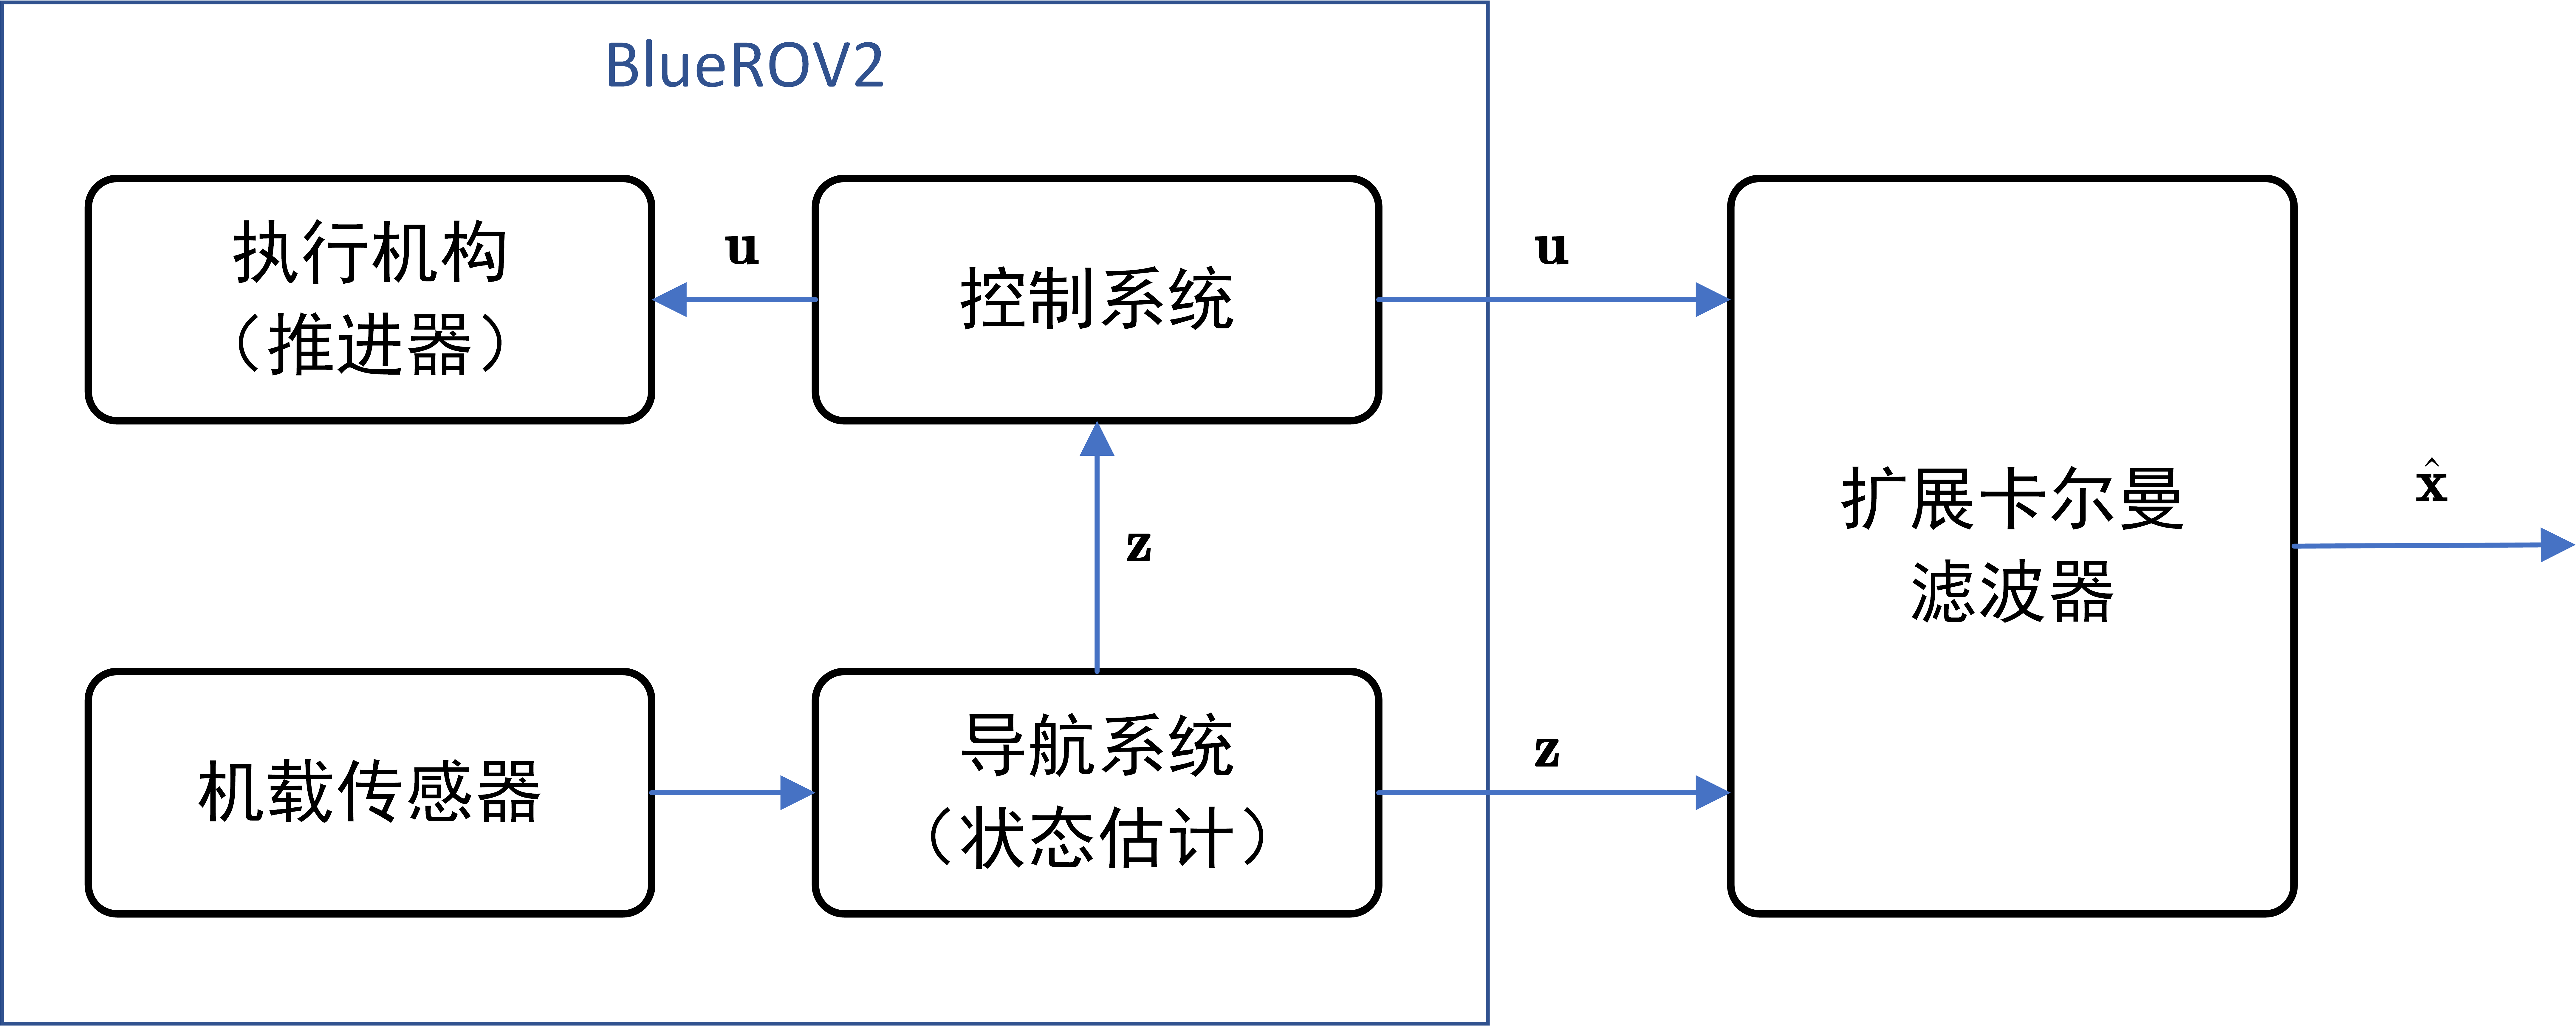
\includegraphics[width=0.7\linewidth]{images/chapter3/卡尔曼滤波辨识流程图.png}
    \caption{扩展卡尔曼滤波器辨识动力学参数流程图}
    \label{f.EKF_ident_frame}
\end{figure}

控制系统内采用传统的PID控制方法,根据预设好的轨迹坐标,设计三个PID控制器分别对水下机器人高度、位置和姿态进行控制,通过PID控制输出BlueROV2导航所需升力、横滚力矩、俯仰力矩、偏航力矩,最后由推力分配矩阵得到各个电机转速的控制信号$\symbf{u}$。PID控制方程为:
\begin{equation}
    u = K_p(x_c-x_r)+K_d\frac{\text{d}(x_c-x_r)}{\text{d}t}+K_i\int_{0}^{t}(x_c-x_r)\text{d}t
\end{equation}
其中,$K_p, K_i, K_d$分别是系统的比例控制系数、微分控制系数和积分控制系数,$x_c$为系统当前状态变量,$x_r$为系统预设状态变量。系统在惯性坐标系下的位姿向量为$\symbf{\eta}=[x,y,z,\phi,\theta,\psi]^T$,则各个位姿分量的控制参数如表\ref{t.PID_params}所示。
\begin{table}[htb]
  \centering
  \caption{BlueROV2各位姿分量PID控制参数}
  \label{t.PID_params}
  \begin{tabular}{cccc}
  \hline
位姿分量 & $K_p$ & $K_d$ & $K_i$ \\
\hline
$x$ & 0.9555 & 1.3650 & -0.3000 \\
$y$ & 0.9555 & 1.3650 & -0.3000 \\
$z$ & -7.8000 & -3.9000 & 5.2000 \\
$\phi$ & 1.6800 & 0.3360 & -2.8000 \\
$\theta$ & 1.6800 & 0.3360 & -2.8000 \\
$\psi$ & 3.2700 & 0.6540 & -5.4500 \\
\hline
\end{tabular}
\end{table}
导航系统中结合了BlueROV2的动力学方程,通过传感器数据测量系统当前状态变量,根据控制输入变量与当前状态测量下一时刻的系统状态。为准确模拟传感器测量误差,本文根据各个传感器测量噪声特点加入噪声以模拟真实的测量环境。扩展卡尔曼滤波器中,根据上述算法更新增广状态向量$\hat{\symbf{x}}$向量,以此得到BlueROV2的动力学模型参数。

扩展卡尔曼滤波器中,需要调增超参数$Q_k$与$R_k$的值,使得卡尔曼滤波器能够较好地模拟实际测量噪声,以此便于模型参数的辨识,通过测试,本文设定卡尔曼滤波器增广状态向量对应的噪声协方差如表所示,其中$P_{ini}$表示增广状态向量的初始协方差,该值会在后续迭代过程中发生改变。

\begin{table}[htb]
  \centering
  \caption{仿真中使用的EKF参数值}
  \label{t.PID_params}
  \zihao{6}
  \begin{tabular}{ccccccccccccc}
  \hline
状态分量 & $x$ & $y$ & $z$ & $\phi$ & $\theta$ & $\psi$ & $u$ & $v$ & $w$ & $p$ & $q$ & $r$ \\
\hline
$P_{ini}$ & 1 & 1 & 1 & 0.1 & 0.1 & 0.1 & 0.1 & 0.1 & 0.1 & 0.1 & 0.1 & 0.1  \\
$Q$ & 0.1 & 0.1 & 0.1 & 0.1 & 0.1 & 0.1 & 0.1 & 0.1 & 0.1 & 0.1 & 0.1 & 0.1  \\
$R$ & 0.01 & 0.01 & 0.01 & 0.0025 & 0.0025 & 0.0025 & 0.0025 & 0.0025 & 0.0025 & 0.0025 & 0.0025 & 0.0025 \\
\hline
\hline
状态分量 & $X_u$ & $Y_v$ & $Z_w$ & $K_p$ & $M_q$ & $N_r$ & $X_{\dot{u}}$ & $Y_{\dot{v}}$ & $Z_{\dot{w}}$ & $K_{\dot{p}}$ & $M_{\dot{q}}$ & $N_{\dot{r}}$ \\
\hline
$P_{ini}$ & 1 & 1 & 1 & 0.1 & 0.1 & 0.1 & 0.1 & 0.1 & 0.1 & 0.1 & 0.1 & 0.1  \\
$Q$ & 0.1 & 0.1 & 0.1 & 0.1 & 0.1 & 0.1 & 0.1 & 0.1 & 0.1 & 0.1 & 0.1 & 0.1  \\
$R$ & - & - & - & - & - & - & - & - & - & - & - & - \\
\hline
\end{tabular}
\end{table}

\subsection{扩展卡尔曼滤波器辨识结果}

通过仿真,本文对于BlueROV2的附加质量系数、一阶阻尼系数进行辨识,辨识的结果分别如图\ref{f.added_mass_ident}和图\ref{f.damping_ident}所示,通过扩展卡尔曼滤波器矩阵辨识,增广状态向量曲线最后收敛至辨识值,辨识值如表\ref{t.ident_results}所示。通过分析增广状态向量收敛曲线,可以发现与附加质量系数相比,一些阻尼系数,主要是 $Y_v$, $K_p$, $N_r$,在辨识初期表现出更明显的振荡行为,之后才逐渐稳定。这表明这些参数的辨识过程可能对初始扰动或模型耦合更为敏感,或者EKF的调整使得它们需要更长时间来抑制瞬态,而$X_u$, $Z_w$, $M_q$ 的收敛过程相对平滑,振荡不明显。

\begin{figure}[hbt]
    \centering
    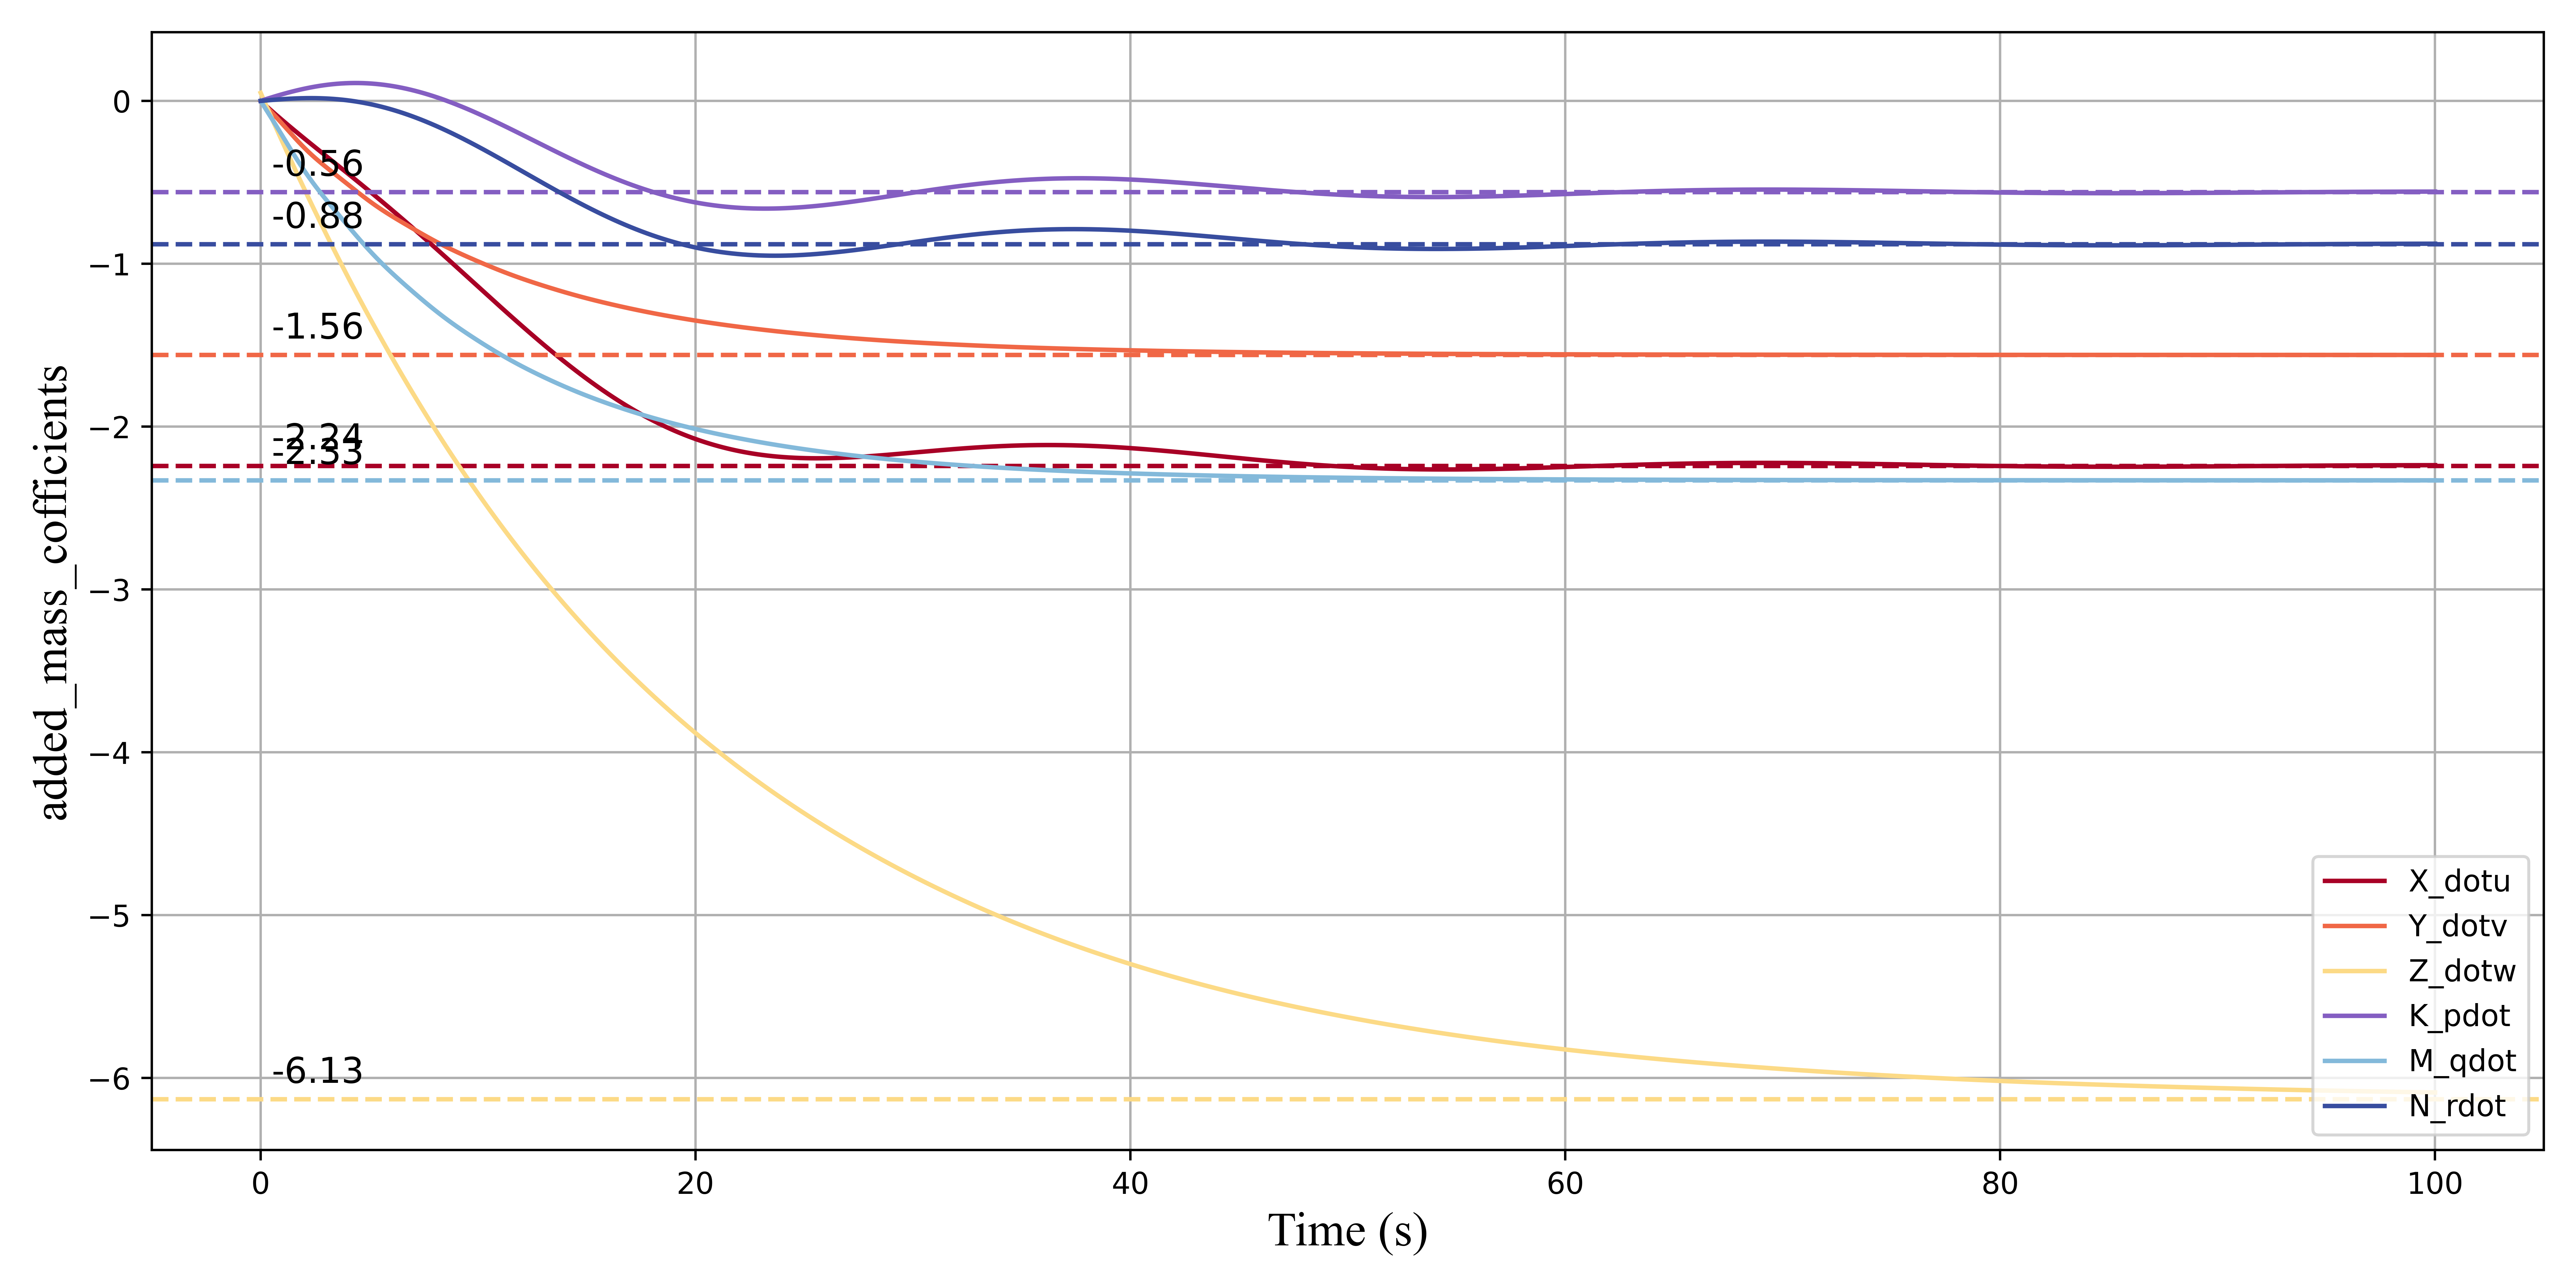
\includegraphics[width=0.8\linewidth]{images/chapter3/附加质量辨识结果.png}
    \caption{BlueROV2附加质量系数辨识}
    \label{f.added_mass_ident}
\end{figure}

\begin{figure}[hbt]
    \centering
    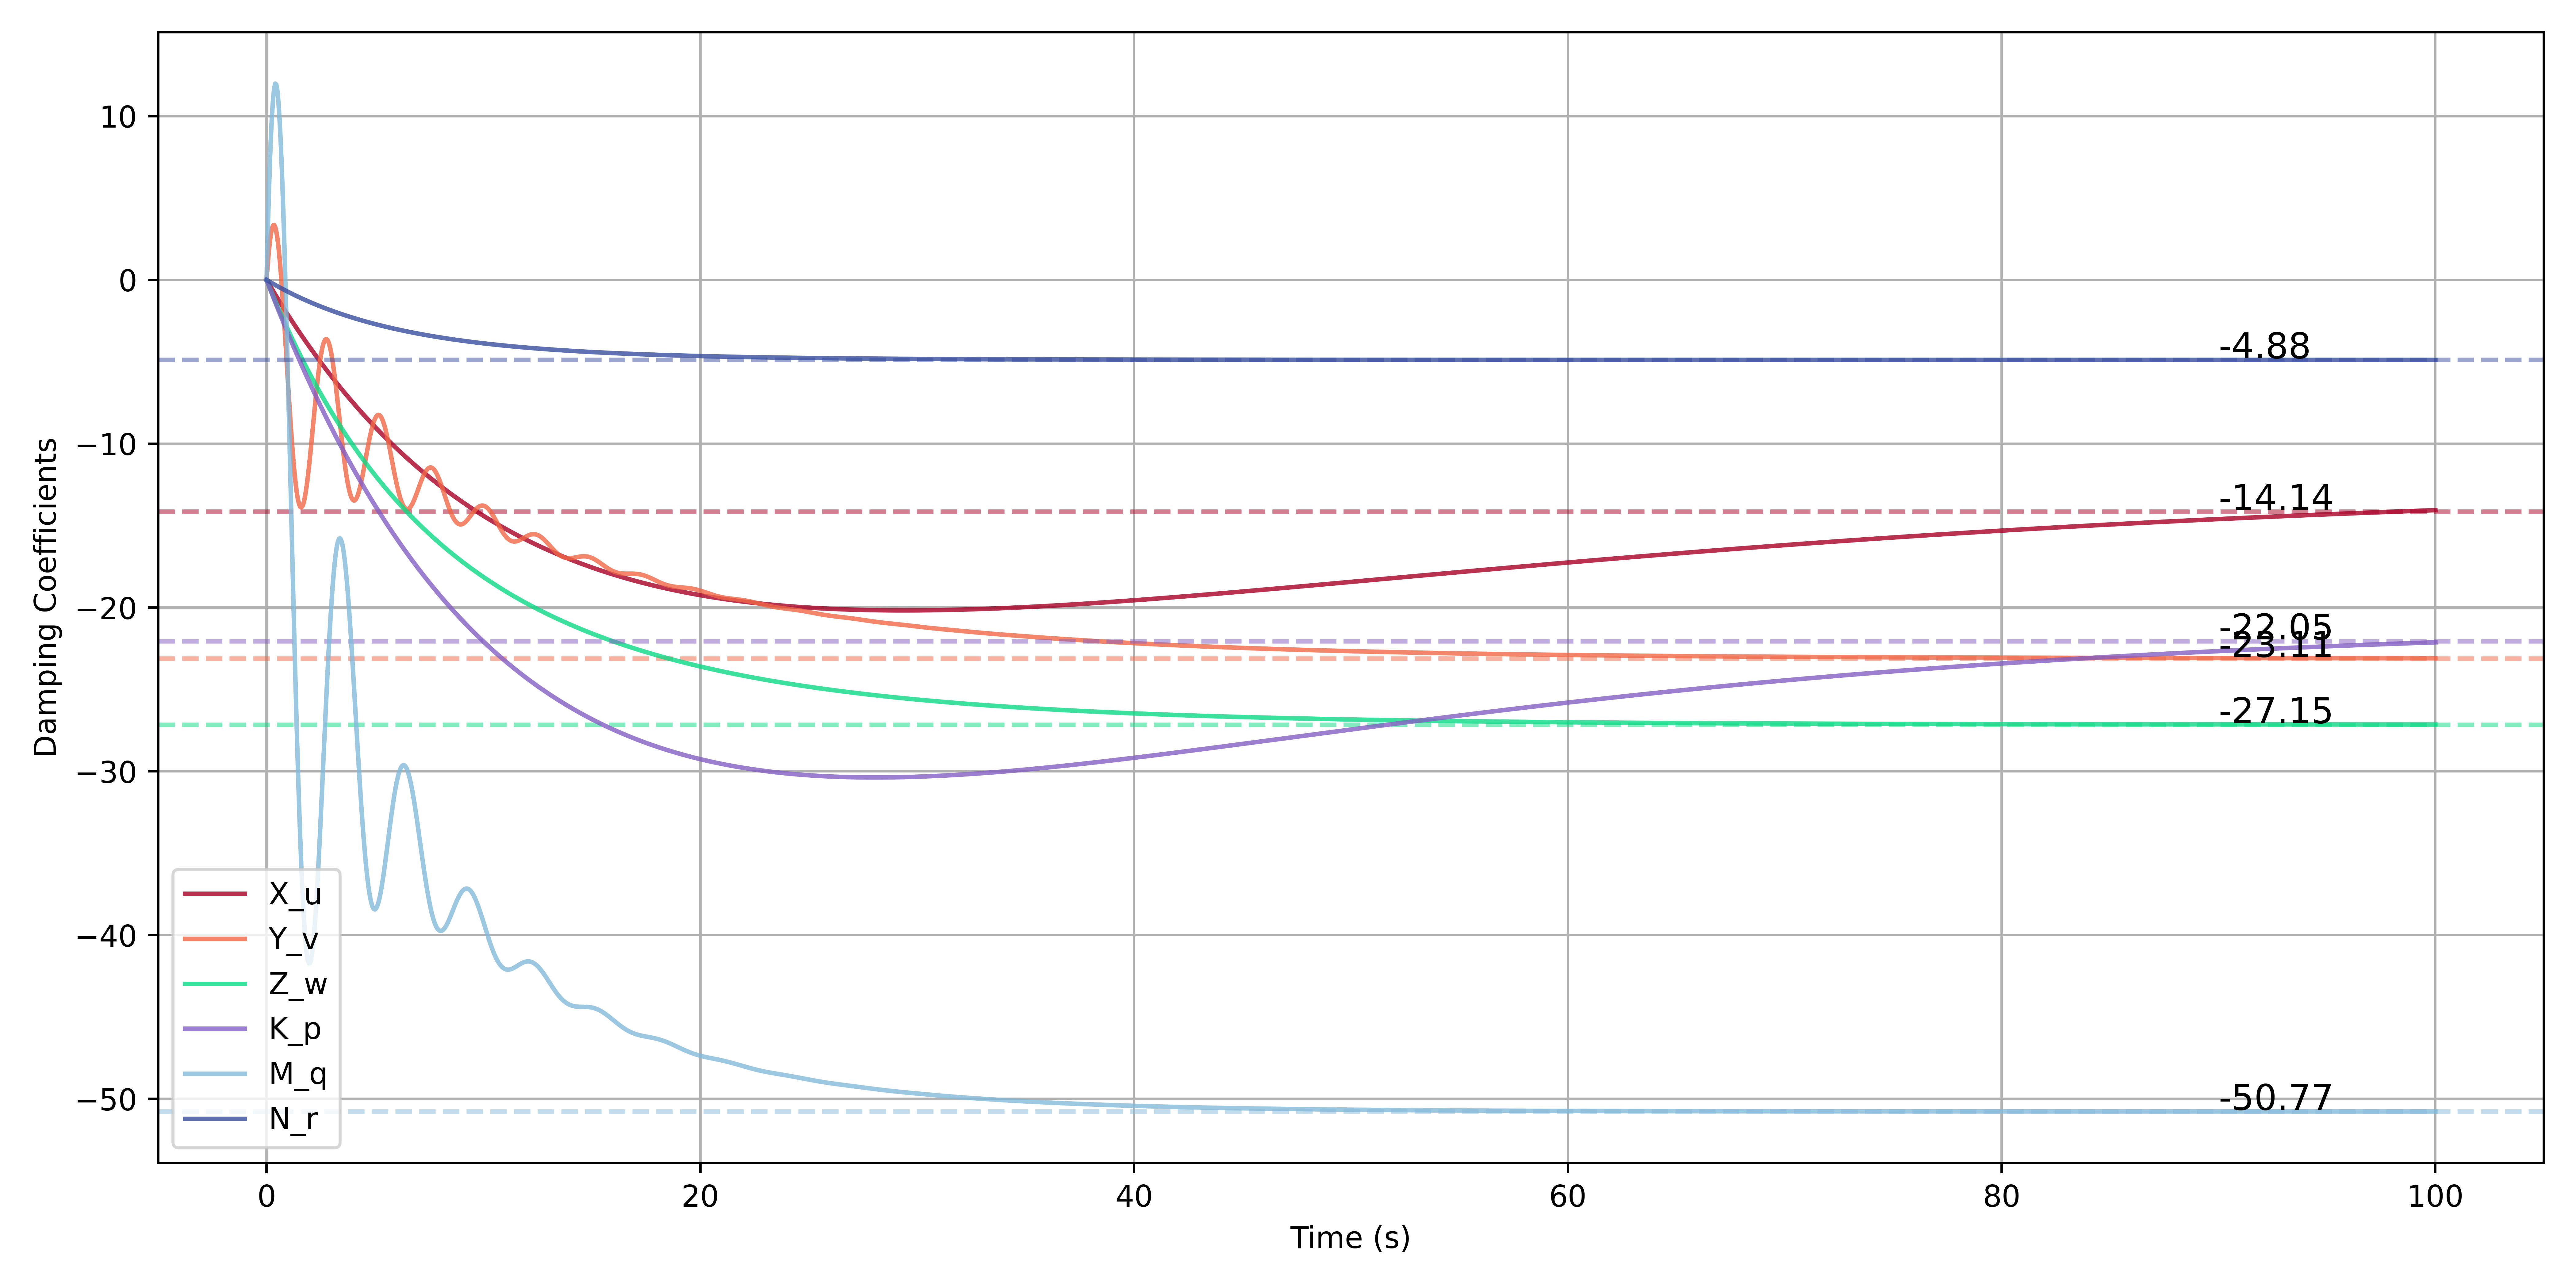
\includegraphics[width=0.8\linewidth]{images/chapter3/阻尼系数辨识结果.png}
    \caption{BlueROV2一阶阻尼系数辨识}
    \label{f.damping_ident}
\end{figure}

\begin{table}[htb]
  \centering
  \caption{扩展卡尔曼滤波器辨识系数结果}
  \label{t.ident_results}
  \begin{tabular}{ccccccc}
  \hline
符号 & $X_{\dot{u}}$ & $Y_{\dot{v}}$ & $Z_{\dot{w}}$ & $K_{\dot{p}}$ & $M_{\dot{q}}$ & $N_{\dot{r}}$ \\
\hline
辨识值  & -2.24  & -1.56 & -6.13  & -0.56 & -2.33 & -0.88   \\
\hline
\hline
符号 & $X_u$ & $Y_v$ & $Z_w$ & $K_p$ & $M_q$ & $N_r$ \\
\hline
辨识值  & -14.14 & -23.11  & -27.15 & -22.05  & -50.77 & -4.88 \\
\hline
\end{tabular}
\end{table}

通过上述仿真结构,本文提取BlueROV2状态向量在已辨识系数下的表现。图\ref{f.EKF_position}和图\ref{f.EKF_vel}分别展示了广义位姿向量$[p_n,p_e,p_d,\phi, \theta, \psi]^T$和广义速度向量$[u,v,w,p,q,r]^T$的实际值和测量值的时间序列曲线,其中实际值为蓝色曲线,表示在控制输入和真实水动力系数下BlueROV2的运动曲线,测量值表示在控制输入和辨识水动力系数下BlueROV2的运动曲线,此外,由于控制输入是对BlueROV2深度坐标和姿态信息$[\phi, \theta,\psi]^T$的控制,其中的绿色曲线表示对应的控制信号。

通过信号对比可以发现,辨识出的系统在深度方向上的速度$w$表现较差,测量值存在噪音明显,与实际值不符,而系统在姿态控制上符合良好,表明该系统能够有效地处理BlueROV2系统的姿态控制,而在位置坐标控制上表现较弱。

\begin{figure}[hbt]
    \centering
    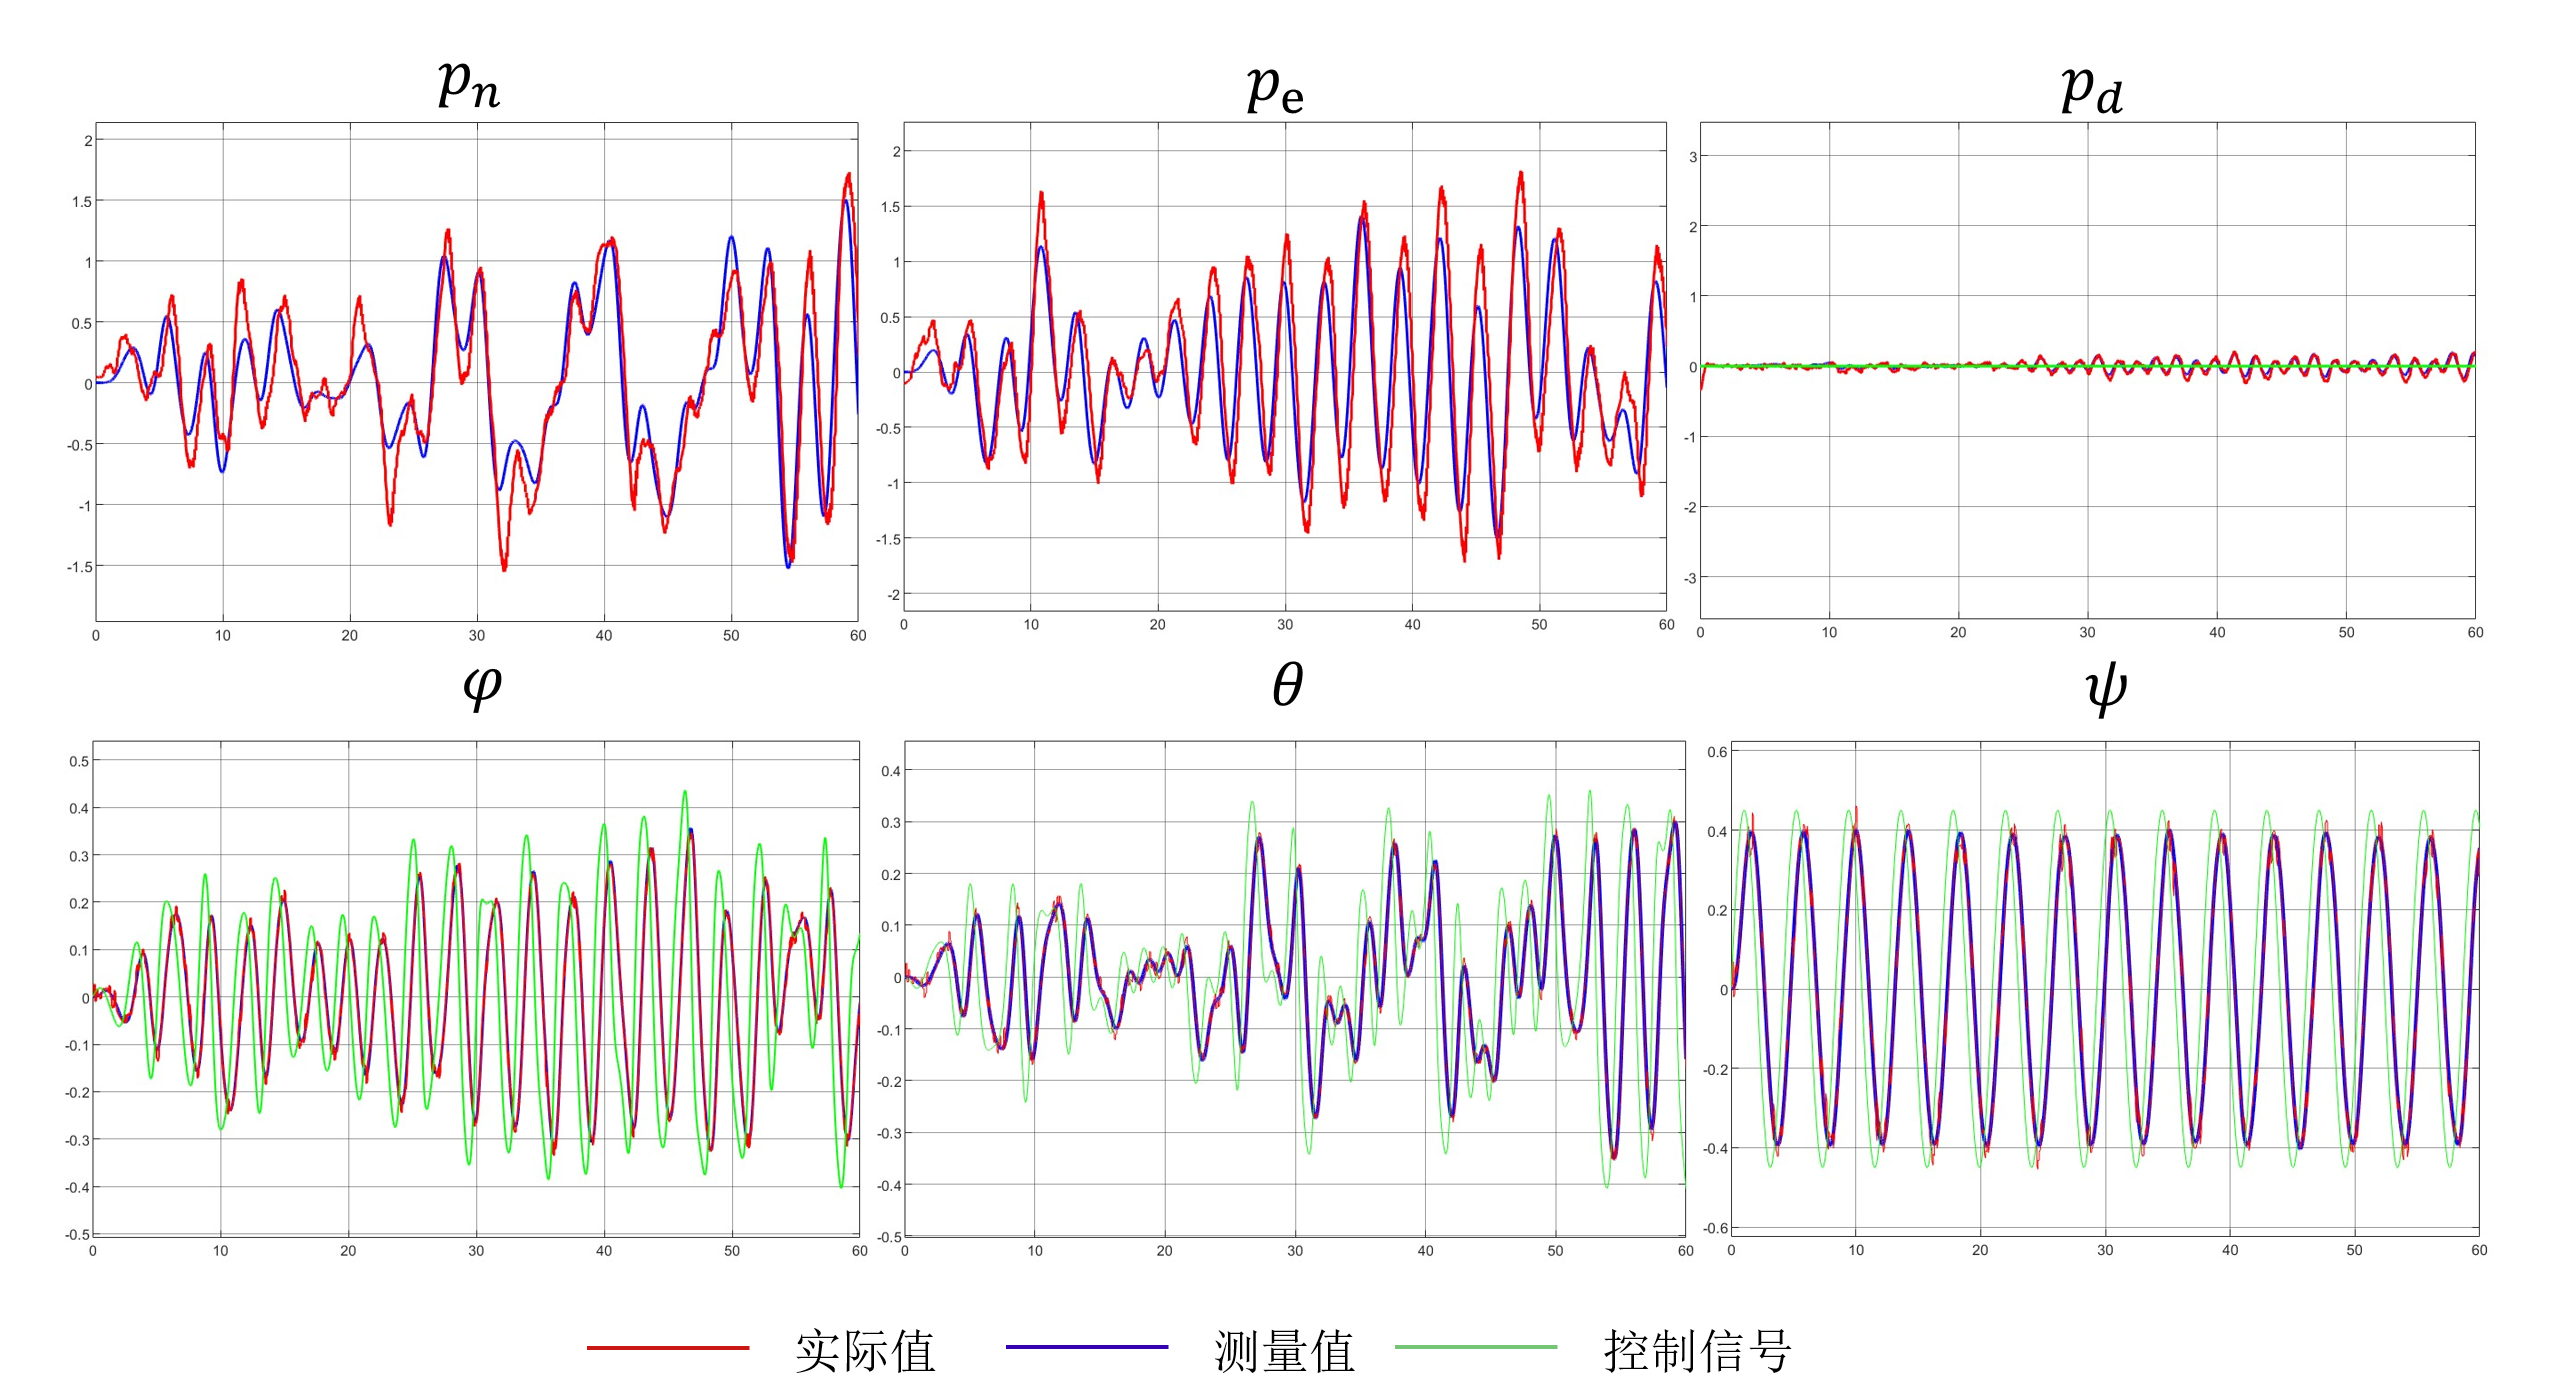
\includegraphics[width=0.8\linewidth]{images/chapter3/EKF_position.png}
    \caption{BlueROV2广义位姿向量辨识效果}
    \label{f.EKF_position}
\end{figure}
\begin{figure}[hbt]
    \centering
    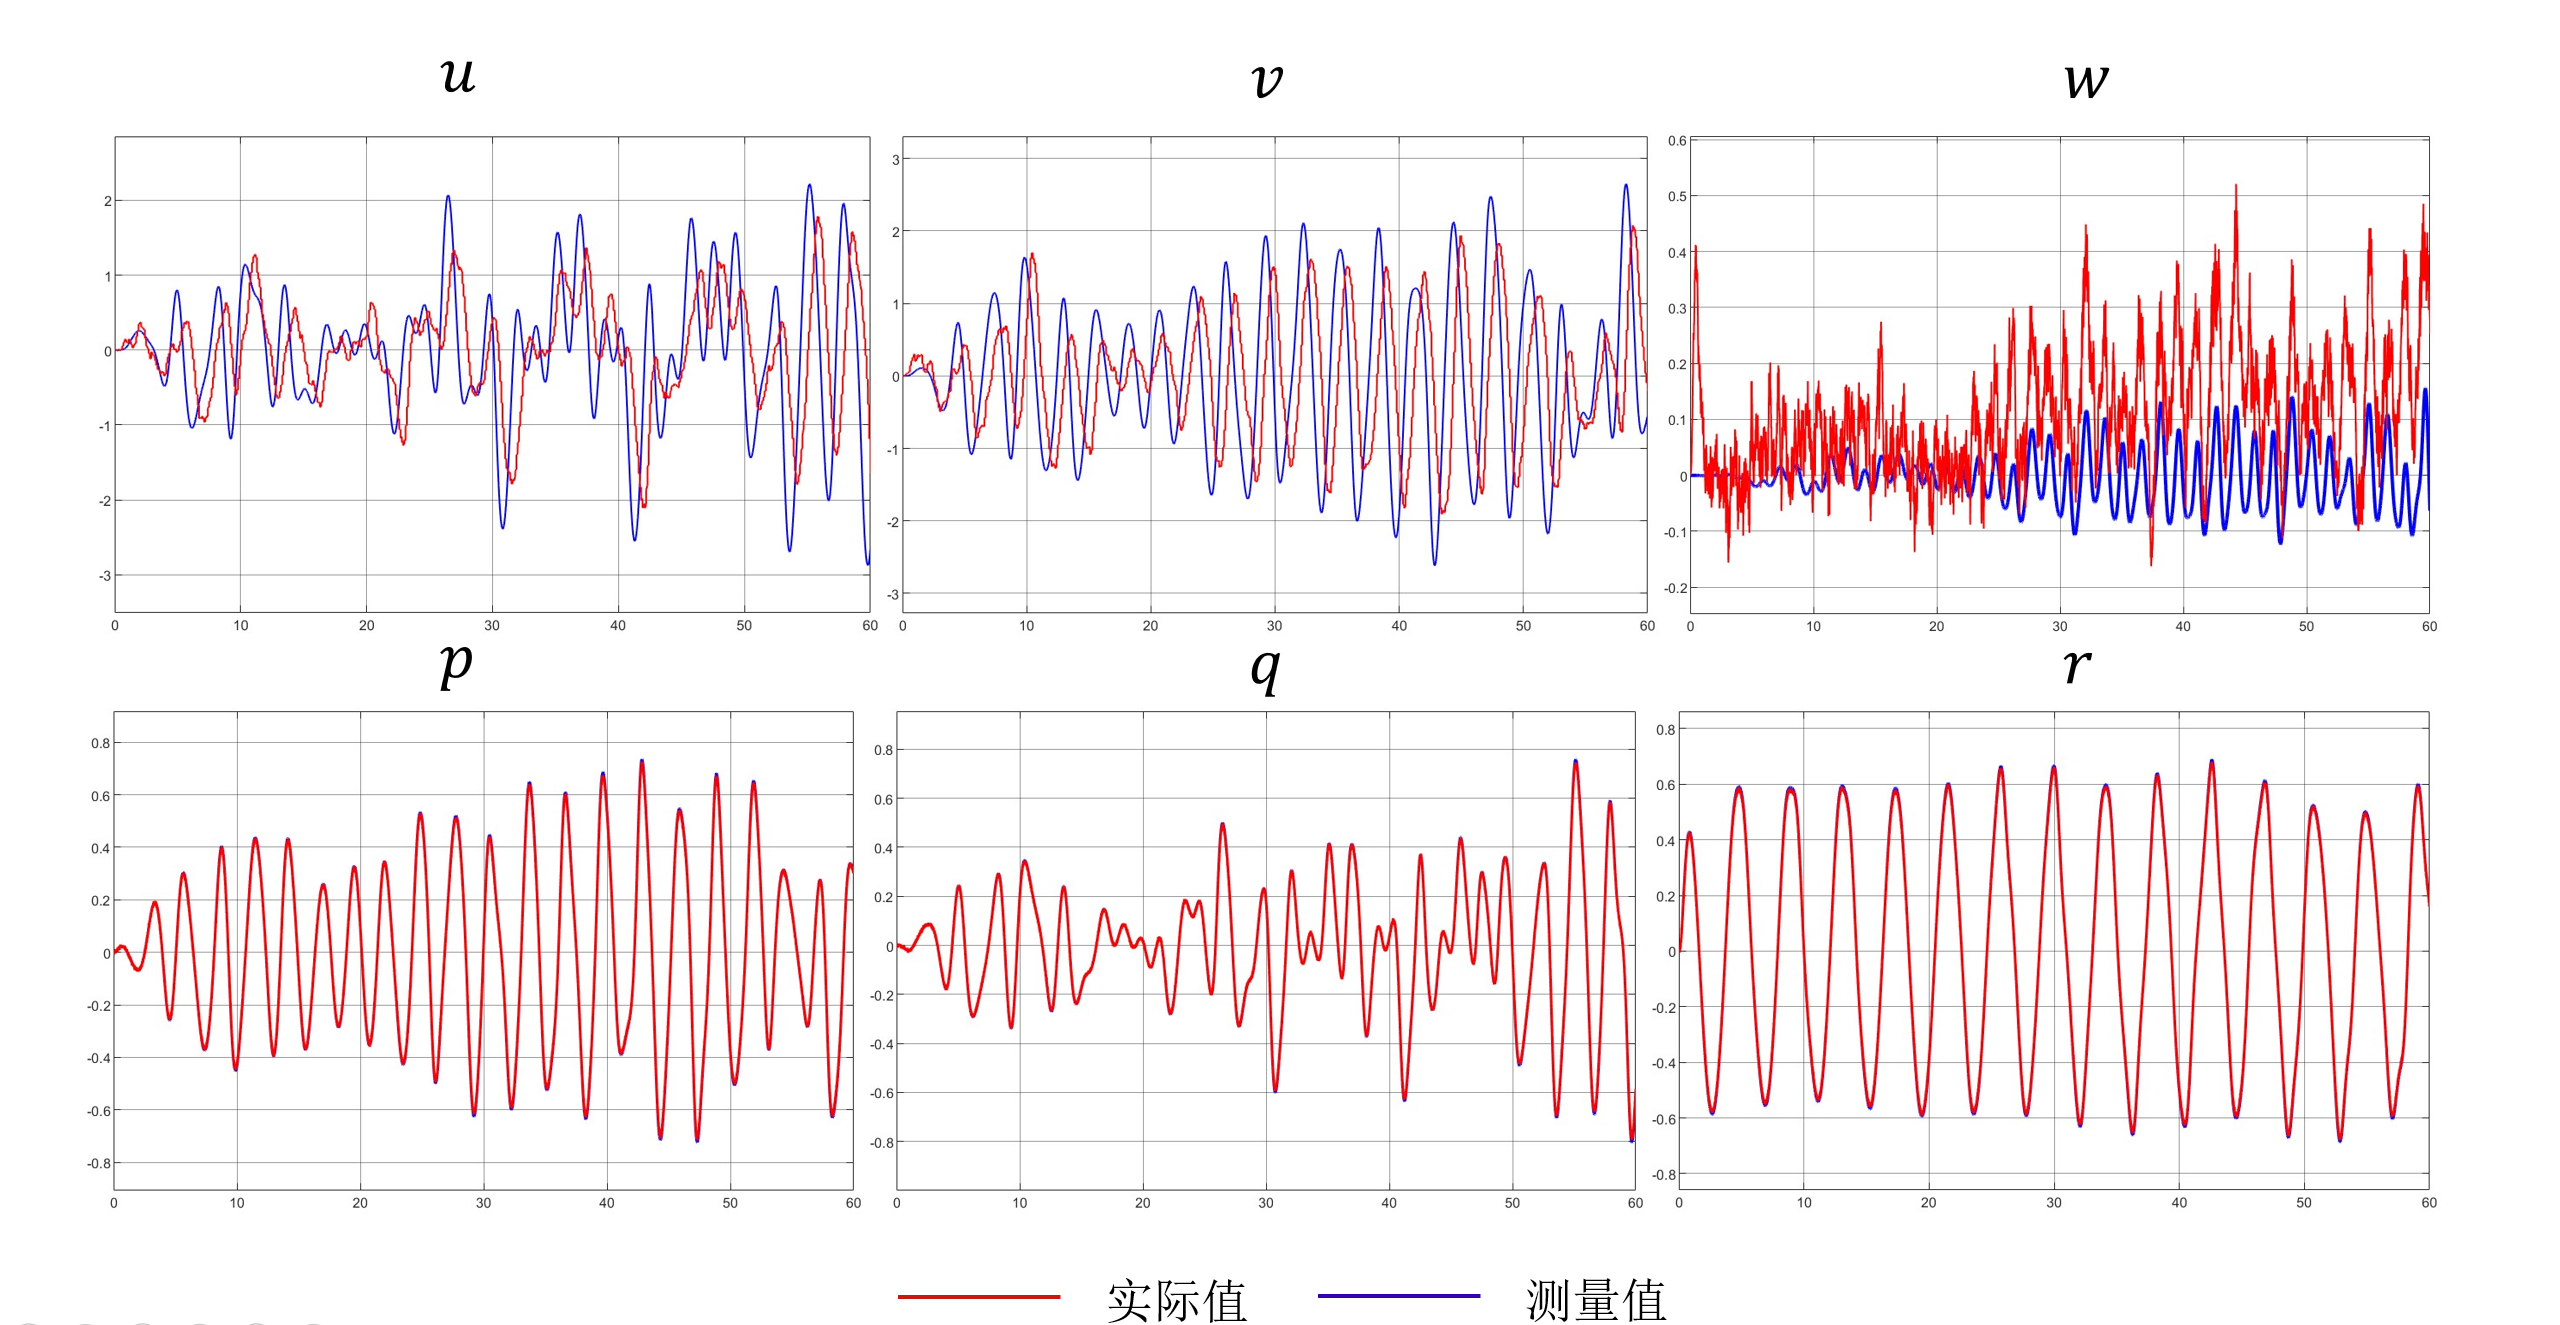
\includegraphics[width=0.8\linewidth]{images/chapter3/EKF_vel.png}
    \caption{BlueROV2广义速度向量辨识效果}
    \label{f.EKF_vel}
\end{figure}

\section{本章小结}

本章节在前一章节完成BlueROV2动力学建模的基础上,通过最小二乘法和扩展卡尔曼滤波方法对BlueROV2动力学模型未知参数进行辨识。考虑到需要辨识的有18个参数,六自由度的动力学方程与参数个数不兼容,故将运动曲线解耦为水平面运动模型与竖直面运动模型分别分析,辨识出水动力系数;而在扩展卡尔曼滤波方法中,通过建立MATLAB/Simulink仿真结构,模拟机载传感器测量噪声和控制信号,建立增广状态向量,完成了动力学参数的辨识,并且将实际值和测量值曲线进行了比较,得到卡尔曼滤波方法的辨识特性。

\newpage
%%%%%%%%%%%%%%%%%%%%%%%%%%%%%%%%表格插入示例%%%%%%%%%%%%%%%%


%%%%%%%%%%%%%%%%%%%%%%%%%%%%%%%%参考文献插入示例%%%%%%%%%%%%%%%%
%!TEX root = ../../csuthesis_main.tex
\chapter{ROV运动控制仿真}
在前面的内容中,本文已经完成 ROV 的动力学建模,并且利用最小二乘算法和卡尔曼滤波算法分别针对ROV的水动力参数进行辨识,本章节使用UUV Simulator仿真平台\cite{Manhaes_2016}构建BlueROV2的仿真实例,具体仿真环境如图\ref{f.simulation_environment}所示,在仿真平台下,通过设定预设轨迹,调整水动力参数,测试两种方法辨识出的水动力系数对于轨迹跟踪的性能影响,以此比较两种辨识算法的优劣势。

\begin{figure}[hbt]
    \centering
    \includegraphics[width=0.8\linewidth]{images/chapter4/simulation_environment.png}
    \caption{UUV Simulator 仿真环境}
    \label{f.simulation_environment}
\end{figure}

\section{UUV Simulator 仿真平台搭建}

UUV Simulator是一款基于Gazebo物理引擎和ROS框架的开源仿真平台,专为水下机器人(如AUV、ROV)及多机器人协作任务设计,其结合了Gazebo的物理仿真能力和ROS的机器人控制框架,构建分层式模块设计。Gazebo插件层提供基于Fossen方程实现水下机器人六自由度动力学仿真,支持推进器推力分配、流体阻力与升力建模,支持模拟真实的传感器数据输出,包括惯性测量单元IMU,GPS测量系统,姿态和航向参考系统(AHRS)等,提供海底地形、沉船场景、动态水流,包括恒定或高斯-马尔可夫过程及水下光照衰减效果,支持自定义海洋环境;ROS框架提供控制算法支持,包含PD/PID、滑模控制(SMC)、反馈线性化等算法,支持动态定位(DP)及轨迹跟踪,提供通信中间件,可以通过ROS Bridge实现Gazebo与ROS的双向通信,允许用户通过ROS话题发布控制指令或订阅传感器数据,提供多机器人协同任务接口,支持水下探测、目标跟踪、干预操作等复杂场景仿真。

本文通过构建ROS节点与话题,搭建BlueROV2在UUV Simulator下的仿真框架如图\ref{f.simulation_framework}所示。首先,由\cs{/world\_ned\_frame\_publisher}节点和\cs{/publish\_world\_models}节点用于初始化系统状态,启动并加载仿真环境以及BlueROV2机器人urdf模型,构建坐标转换TF树,其次,\cs{/gazebo}节点代表Gazebo物理引擎,基于物理规律持续更新 BlueROV2 的状态,并在\cs{/bluerov2/pose\_gt}上发布其地面真实位姿,\cs{/bluerov2\_mpc}\cs{\_node}节点通过订阅该话题以获取机器人当前状态,以此作为输入,根据其内部逻辑包含的MPC 算法计算出对 6 个推进器中每一个所需的控制变量,并将控制变量发布到相应的\cs{/bluerov2/thrusters/N/input}话题,最后\cs{/gazebo}节点接收这些输入指令,并在物理仿真中对 BlueROV2 模型施加相应的力/力矩,以此完成物理更新和状态的反馈,构成闭环系统。

\begin{figure}[hbt]
    \centering
    \includegraphics[width=0.8\linewidth]{images/chapter4/仿真流程.png}
    \caption{BlueROV2仿真结构图}
    \label{f.simulation_framework}
\end{figure}

\section{MPC控制器设计与介绍}
本文采取MPC对BlueROV2进行控制,模型预测控制(MPC)是一种先进的过程控制方法,它利用系统的动态模型来预测未来的行为,并基于这些预测来计算最优的控制动作,它通过递归求解OCPs来确定控制动作,并在控制过程中满足系统约束。相较于PID和其他控制算法,MPC算法融合了模型的系统状态方程,更加符合物理规律,且能够有效考虑物理因素限制和系统约束。\cite{huDisturbanceObserverBasedModel2024}

\begin{figure}[hbt]
    \centering
    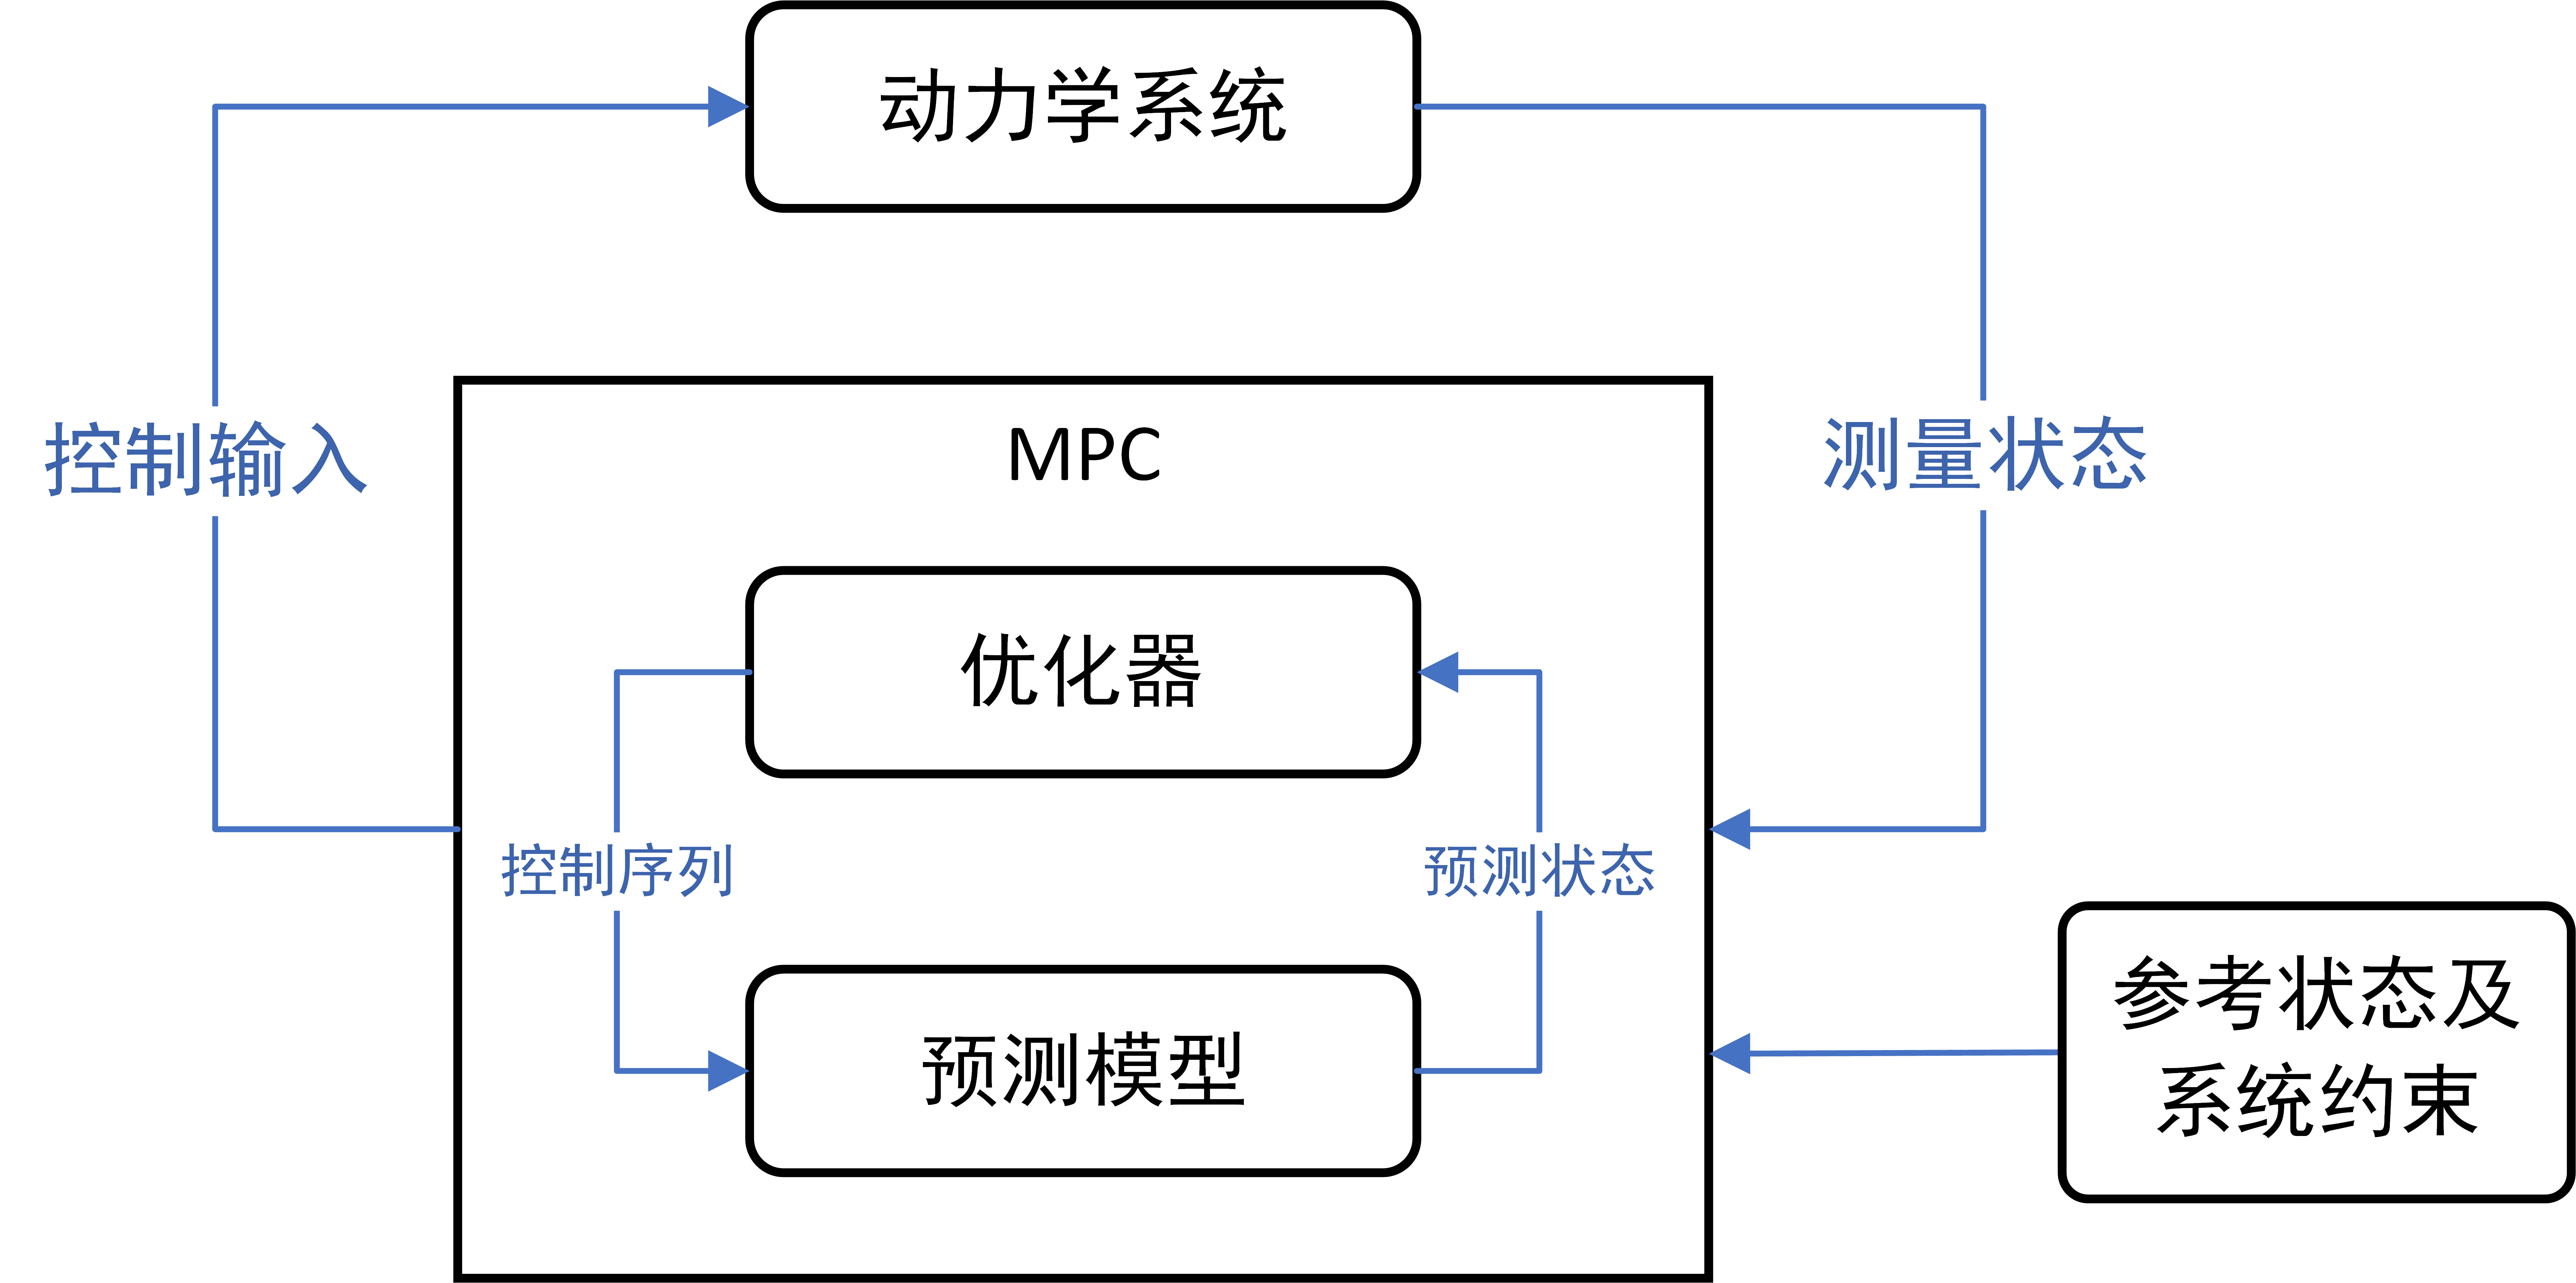
\includegraphics[width=0.8\linewidth]{images/chapter4/MPC控制闭环图.png}
    \caption{MPC控制回路}
    \label{f.MPC_control_loop}
\end{figure}

MPC主要包含两个部分,预测模型和优化器,MPC的控制回路如图\ref{f.MPC_control_loop}所示。在MPC控制回路中,它从动态系统中接收参考状态、系统约束和测量状态,并将控制输入输反馈回动力学系统。MPC根据预测模型在一定范围内的控制输入序列计算预测输出,而优化器解决二次规划( QP )问题:

\begin{equation}
\begin{aligned}
 & \min_{U,X}\int_{t=0}^T 
 \begin{Vmatrix}
     h(x(t),u(t))-y_{ref}
 \end{Vmatrix}_Q^2dt +
  \begin{Vmatrix}
     h(x(T))-y_{N,ref}
 \end{Vmatrix}_{Q_N}^2
 \\
& \text{subject to} \quad \dot{x}=f(x(t),u(t)); \\
& u(t) \in \mathbb{U} \\
& x(t) \in \mathbb{X} \\
& x(0) = x(t_0)
\end{aligned}
\end{equation}

其中$u(t)$和$x(t)$分别表示$t$时刻的控制输入和系统状态;$T$是预测范围,代表向前预测的时间步数;$y_{ref}$和$y_{N,ref}$分别为预测时域和终终点参考状态中的阶段参考状态;$Q$和$Q_N$是阶段状态和终点状态的权重矩阵;$F(\cdot )$和$h(\cdot )$分别为预测模型和系统输出函数;$\mathbb{U}$和$\mathbb{X}$是控制输入和系统状态的约束。

要调整 MPC,需要遵循几个重要步骤。首先,选择控制范围$T$,考虑权衡控制性能和计算负担。为了找到一个平衡这些因素的最优值,水平在模拟过程中逐步增加,并在评估改善控制性能的同时保持 MPC 的实时运行。此外,MPC 允许通过将矩阵$\symbf{Q}$中的权重因子分配给每个目标来确定多个控制目标的优先级。在这个特殊的工作中,偏航角$\psi $被赋予了最高的优先级,其次是位置状态$x, y, z$。终端成本与在预测范围的末端的系统的最终状态有关。终端状态$Q_N$处的加权矩阵反映了达到期望的稳态或目标的相对意义。权重越高,表示越强调达到所需的终端状态。本工作中为保证控制器稳定性,$Q_N$被设置为等于 $\symbf{Q}$ 中的值,以提供较少的激进控制。

\section{轨迹跟踪仿真验证}

通过前文所述内容,本文已搭建起BlueROV2的动力学模型,通过最小二乘法和扩展卡尔曼滤波器辨识出两组水动力参数,为了比较两个算法在动力学模型辨识上的优劣,本文通过设计不同的轨迹跟踪任务以测试两组系数在实际工作中的表现。

\subsection{仿真参数设置}

本章节根据表\ref{t.physical_params}设置BlueROV2的物理参数,通过URDF文件定义BlueROV2模型并导入UUV Simulator中。表\ref{t.MPC_params}列出了MPC相关参数,预测视界为60,采样时间为0.05s,系统向前推测3s。

\begin{table}[htb]
  \centering
  \caption{MPC控制参数表}
  \zihao{5}
  \label{t.MPC_params}
  \begin{tabular}{cl}
  \hline
参数名 & 参数值\\
\hline
预测视界 & 60s \\
采样间隔 & 0.05s \\
$Q$      & [350, 350, 350, 10, 10, 150, 10, 10, 10, 10, 10, 10, 15, 15, 15, 0.5] \\
$Q_N$   & [350, 350, 350, 10, 10, 150, 10, 10, 10, 10, 10, 10]  \\
OCP时间 & 7ms \\
\hline
\end{tabular}
\end{table}

\subsection{圆形轨迹跟踪仿真验证}

本章节设置圆形曲线作为参考轨迹,使BlueROV2从初始位置$[0,0,-0.5]\text{m}$处出发,沿参考轨迹做绕行运动,定义圆形曲线方程为:
\begin{equation}
    [x_r, y_r, z_r]^T = \left\{\begin{matrix}
  -R\cos(\frac{tv}{R}) + x_0 \\
  -R\sin(\frac{tv}{R}) + y_0 \\
  z_0 
\end{matrix}\right.
\end{equation}
定义绕行偏航角方程为:
\begin{equation}
    \psi_r = \frac{tv}{R}-0.5\pi
\end{equation}
其中,$x_r,y_r, z_r,\psi_r$为参考点的坐标值和参考点处的参考偏航角,$R$为圆形半径,$x_0,y_0,z_0$为初始位置坐标,$v$为期望绕行速度,曲线设置满足$x_0=y_0=0$,$z_0=-20\text{m}$,$R=2\text{m}$,$v=1.5\text{m/s}$。

将扩展卡尔曼滤波器辨识出的水动力参数代入轨道追踪控制框架,在其轨迹收敛后,得到其轨迹跟踪曲线与位置跟踪误差分别如图\ref{f.circle_track_traj}和图\ref{f.circle_track_error}所示。

\begin{figure}[hbt]
    \centering
    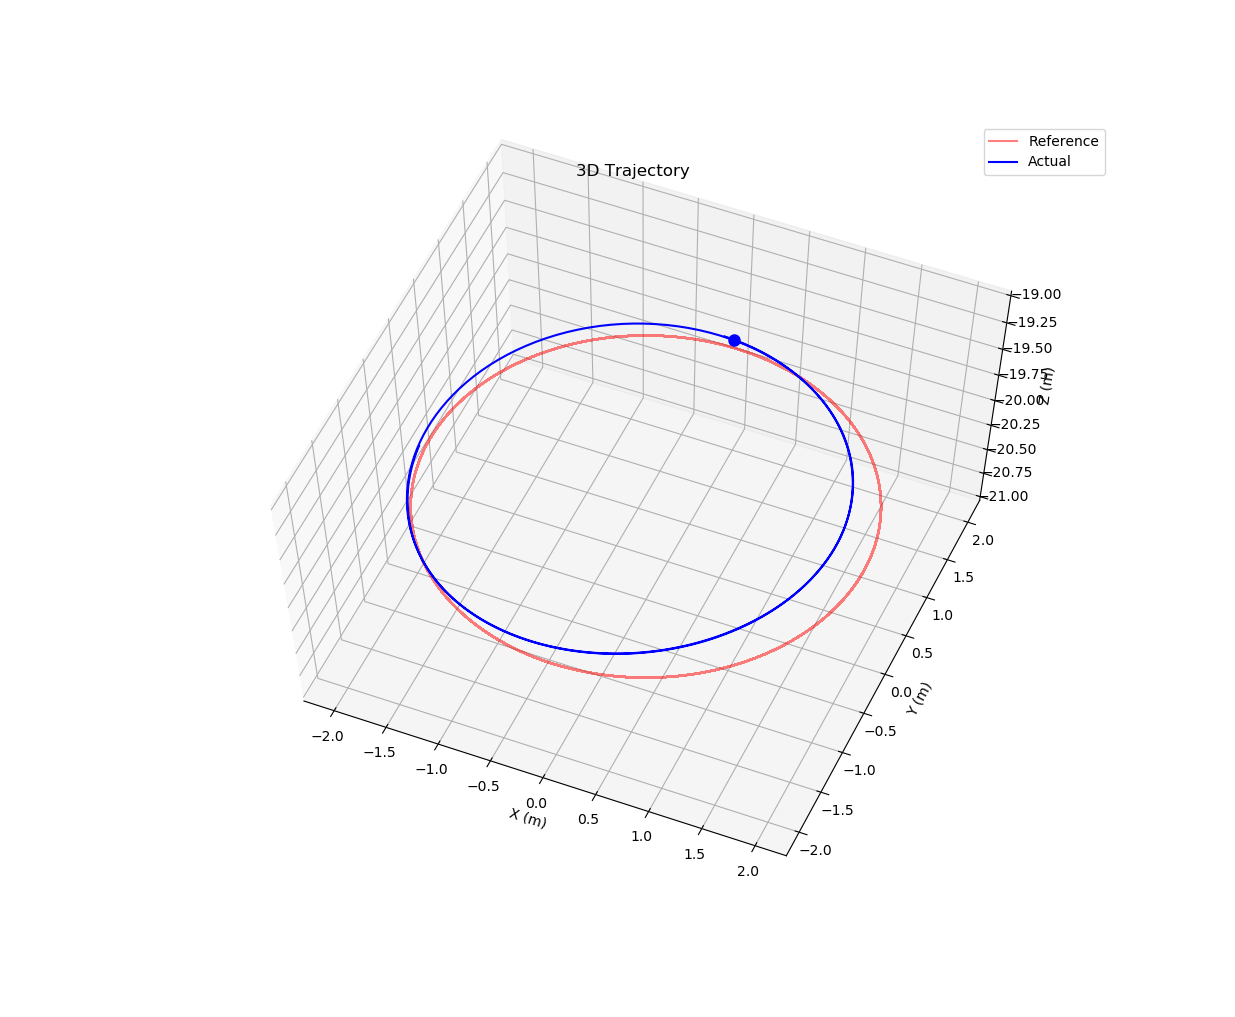
\includegraphics[width=0.8\linewidth]{images/chapter4/circle_track_traj.png}
    \caption{EKF辨识系数下圆形轨迹跟踪曲线}
    \label{f.circle_track_traj}
\end{figure}
\begin{figure}[hbt]
    \centering
    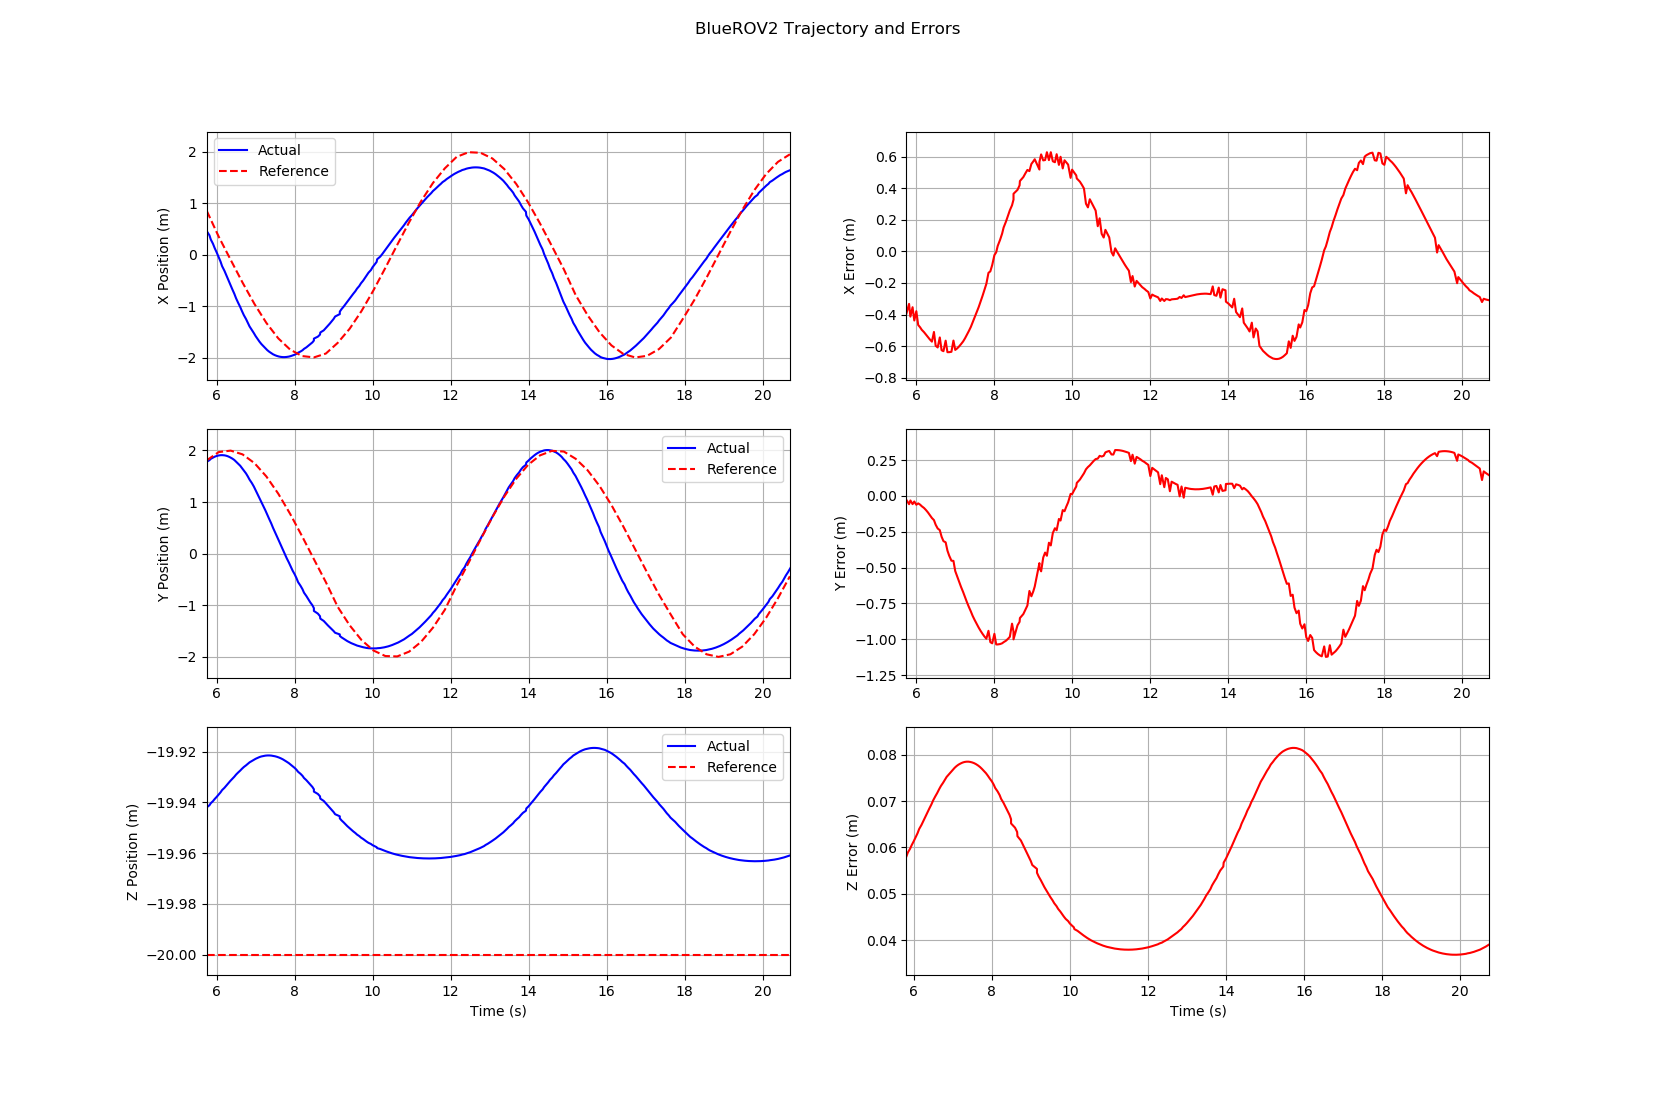
\includegraphics[width=0.8\linewidth]{images/chapter4/circle_traj_error.png}
    \caption{EKF辨识系数下圆形轨迹跟踪误差}
    \label{f.circle_track_error}
\end{figure}

将最小二乘算法辨识出的水动力参数代入轨道追踪控制框架,在其轨迹收敛后,得到其轨迹跟踪曲线与位置跟踪误差分别如图\ref{f.ls_circle_track_traj}和图\ref{f.ls_circle_track_error}所示。

\begin{figure}[hbt]
    \centering
    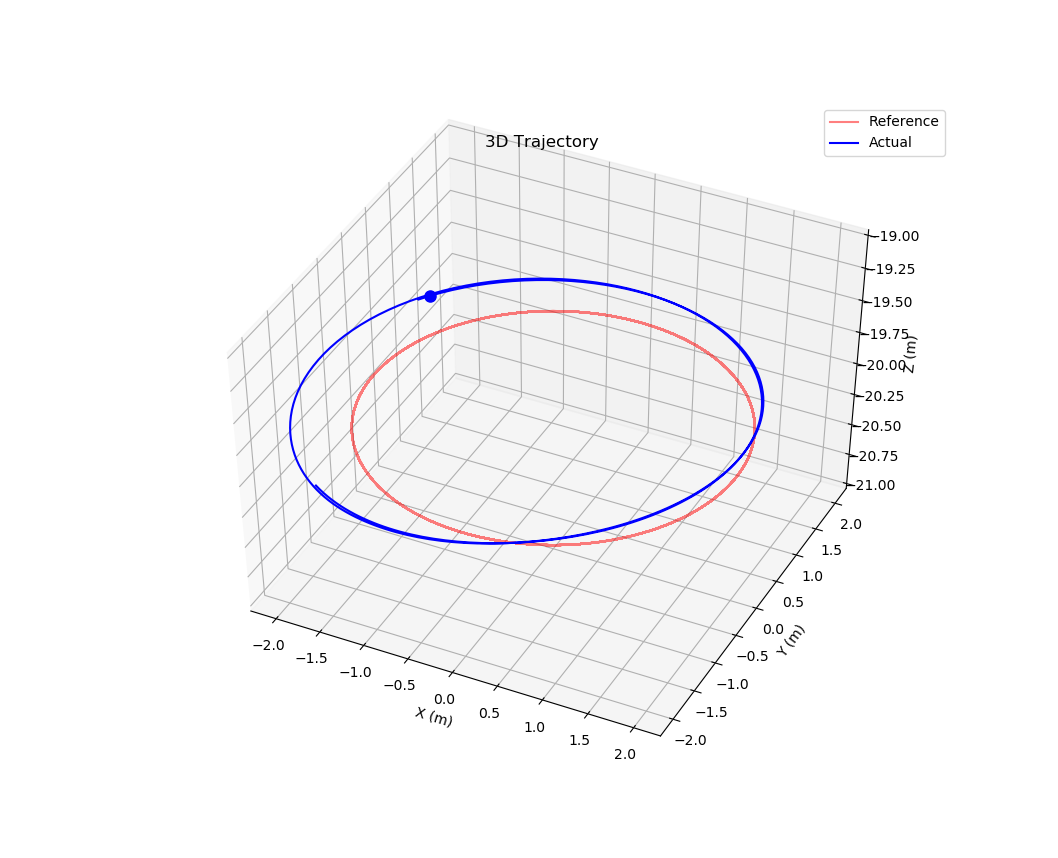
\includegraphics[width=0.8\linewidth]{images/chapter4/ls_circle_traj.png}
    \caption{最小二乘辨识系数下圆形轨迹跟踪曲线}
    \label{f.ls_circle_track_traj}
\end{figure}
\begin{figure}[hbt]
    \centering
    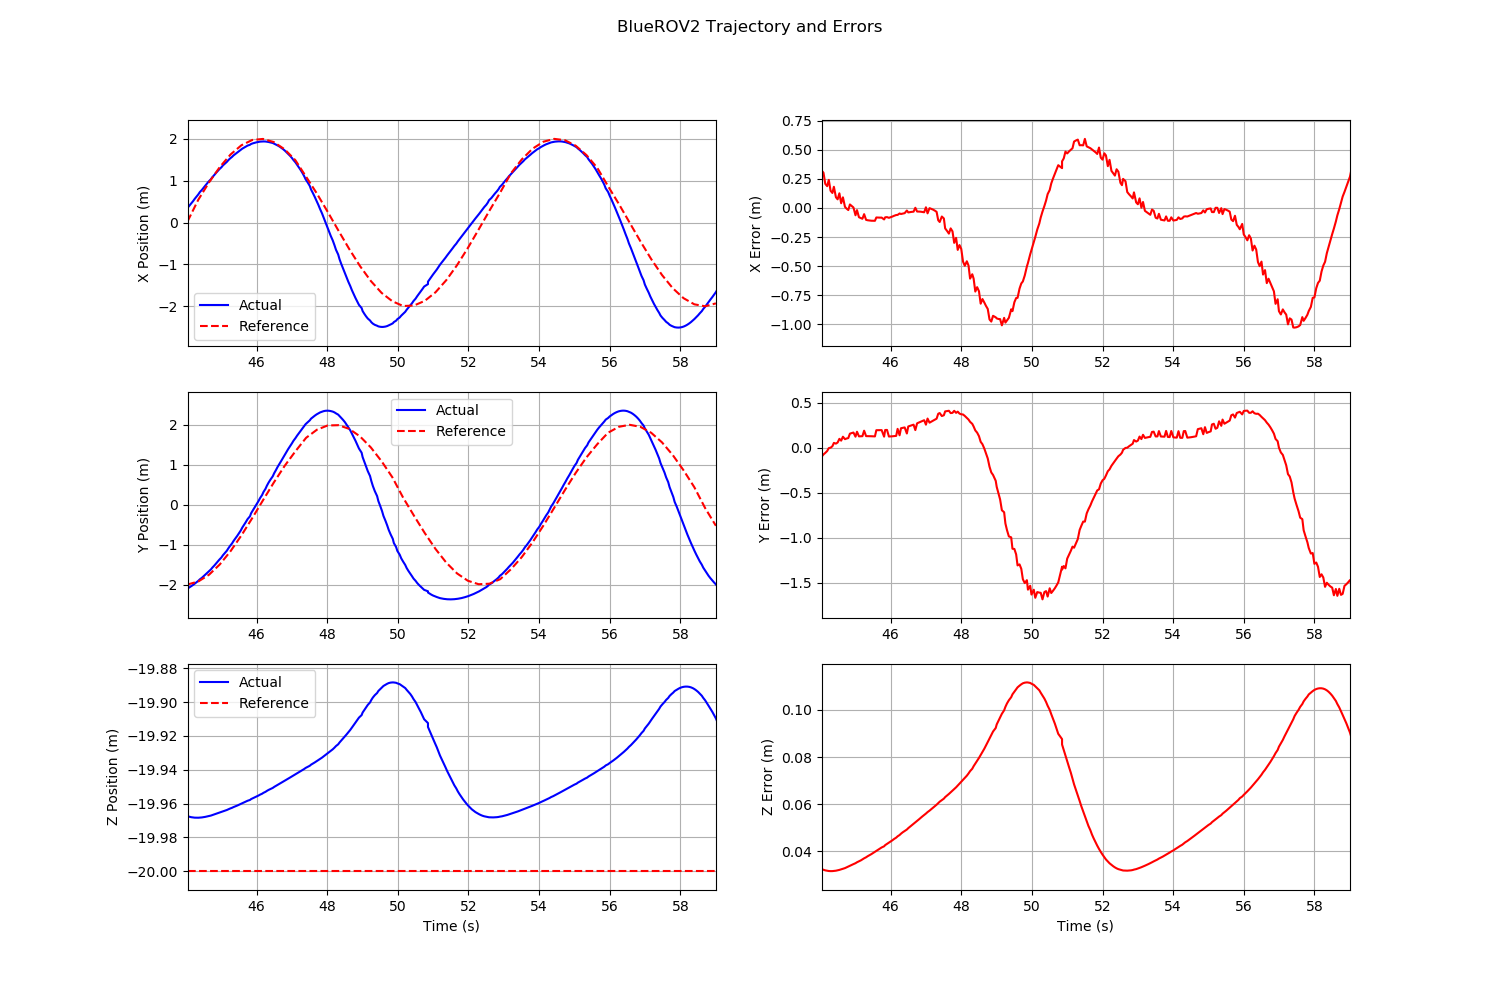
\includegraphics[width=0.8\linewidth]{images/chapter4/ls_circle_error.png}
    \caption{最小二乘辨识系数下圆形轨迹跟踪误差}
    \label{f.ls_circle_track_error}
\end{figure}

通过对比可以看出,最小二乘辨识系数下的圆形轨迹跟踪相较于参考点的超调量大,最大误差占位置变化曲线峰值的25\%,而EKF辨识系数下的圆形轨迹跟踪能更准确地拟合参考轨迹,其在$x$方向上的轨迹跟踪误差依然达到25\%的占比,但是在$Y$方向上的轨迹跟踪误差仅达12\%,同时,两个辨识方法辨识出的系数在$z$方向上的深度控制均有较好的表现。

\subsection{双纽线轨迹跟踪仿真验证}

本章节设置双纽线为参考轨迹,使BlueROV2从初始位置$[0,0,-0.5]\text{m}$处出发,沿参考轨迹做绕行运动,定义双纽线方程为:

\begin{equation}
    [x_r,y_r,z_r]^T=\left\{\begin{matrix}
        A\cos(ft)+x_0 \\
        A\sin(ft)\cos(ft)+y_0 \\
        z_0
    \end{matrix}\right.
\end{equation}
其中,$A$为双纽线长轴距离,$f$为环绕频率,曲线设置满足$A=2m$,$f=0.5s^{-1}$,采样频率为20Hz。

将扩展卡尔曼滤波器辨识出的水动力参数代入轨迹追踪控制框架,在其轨迹收敛后,得到其轨迹跟踪曲线与位置跟踪误差分别如图所示。

\begin{figure}[hbt]
    \centering
    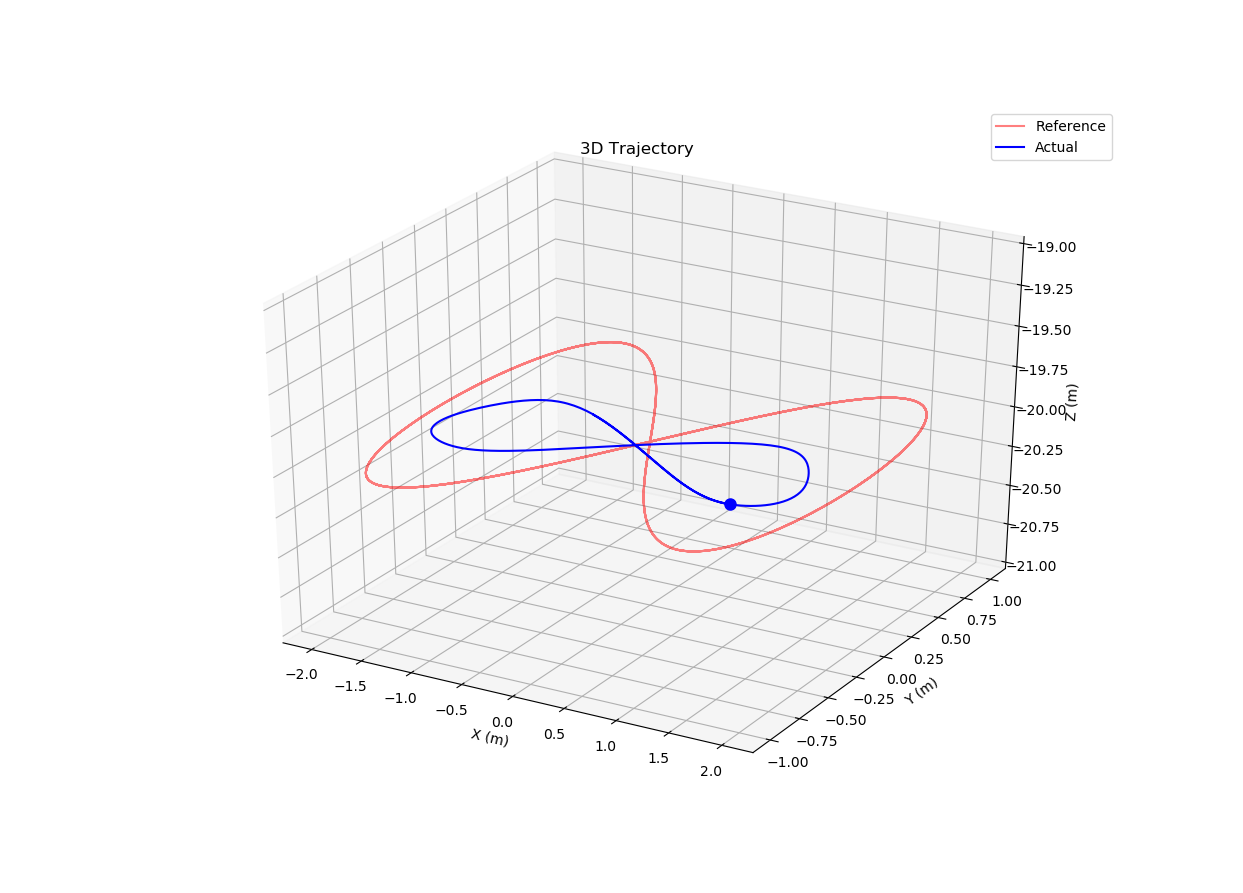
\includegraphics[width=0.8\linewidth]{images/chapter4/lem_traj.png}
    \caption{EKF辨识系数下双纽线轨迹跟踪曲线}
    \label{f.lem_track_traj}
\end{figure}
\begin{figure}[hbt]
    \centering
    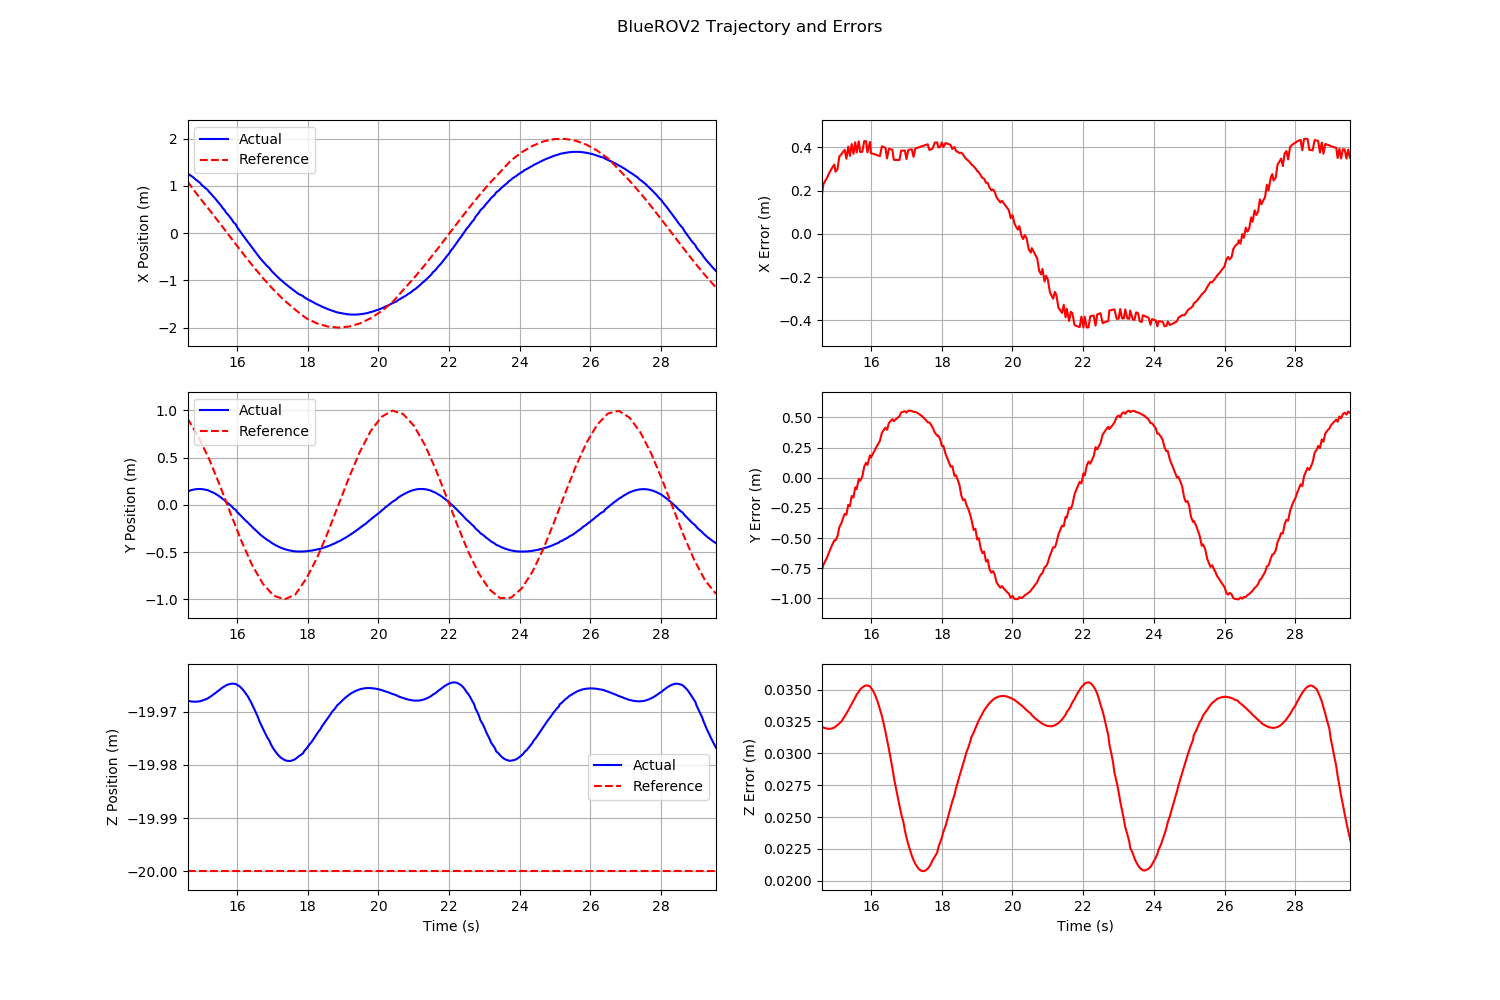
\includegraphics[width=0.8\linewidth]{images/chapter4/lem_error.png}
    \caption{EKF辨识系数下双纽线轨迹跟踪误差}
    \label{f.lem_track_error}
\end{figure}

将最小二乘算法辨识出的水动力参数代入轨迹追踪控制框架,在其轨迹收敛后,得到其轨迹跟踪曲线与位置跟踪误差分别如图\ref{f.lem_track_traj}和图\ref{f.lem_track_error}所示。

\begin{figure}[hbt]
    \centering
    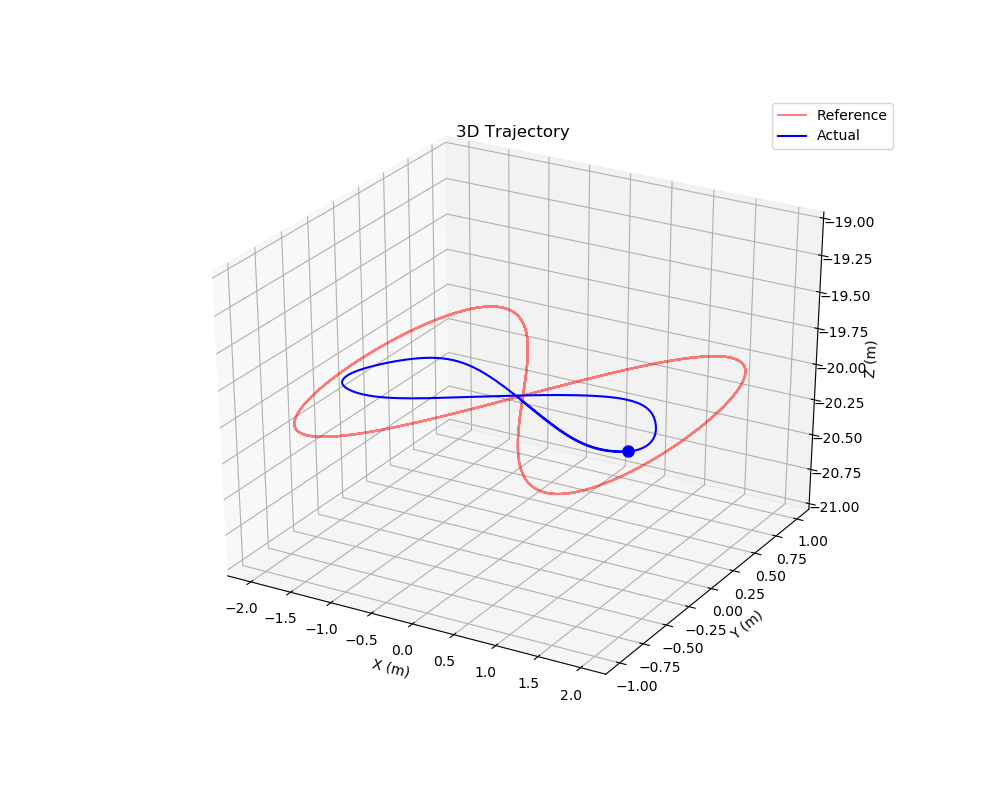
\includegraphics[width=0.8\linewidth]{images/chapter4/ls_lem_traj.png}
    \caption{最小二乘辨识系数下双纽线轨迹跟踪曲线}
    \label{f.lem_track_traj}
\end{figure}
\begin{figure}[hbt]
    \centering
    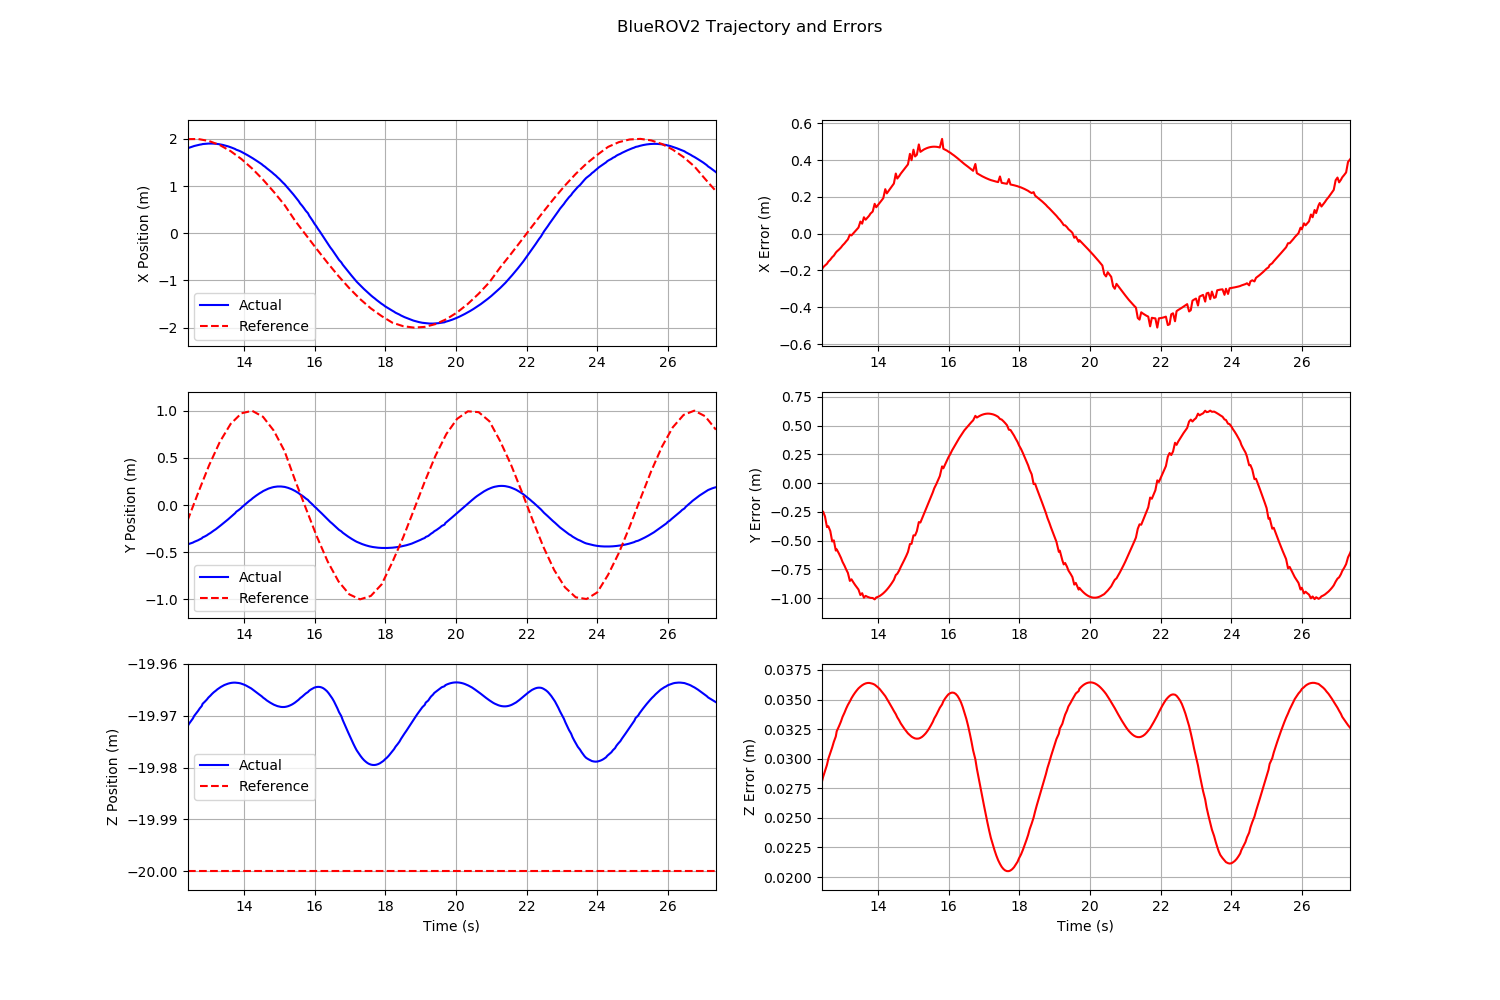
\includegraphics[width=0.8\linewidth]{images/chapter4/ls_lem_error.png}
    \caption{最小二乘辨识系数下双纽线轨迹跟踪误差}
    \label{f.lem_track_error}
\end{figure}

通过对比可以看出,最小二乘和EKF辨识出的系数,在双纽线轨迹跟踪上的表现均不如圆形轨迹跟踪,且尤其在$y$轴方向上误差较大,而在$z$轴方向上均能保持较好的深度控制。此外,在$x$轴方向上,二者最大误差均达到0.4,占参考轨迹最大峰值的25\%,可以认为两者在更为复杂情况下的轨迹跟踪上较无显著差别。

\section{本章小结}

本章节在前一章节辨识水动力参数的基础上,通过UUV Simulator仿真平台,实现了MPC控制器,设计BlueROV2的轨迹跟踪任务。分别设计了圆形和双纽线形两种参考轨迹,再分别代入由最小二乘系数辨识和由扩展卡尔曼滤波器辨识出的水动力参数,分析其轨迹跟踪曲线及误差表现,发现在参考轨迹为圆形时,基于扩展卡尔曼滤波器的轨迹跟踪误差较小,表现良好;而两组水动力系数在双纽线形更为复杂的情况下轨迹跟踪表现并无显著差异。

\newpage




%%%%%%%%%%%%%%%%%%%%%%%%%%%%%%%%参考文献插入示例%%%%%%%%%%%%%%%%

%%%%%%%%%%%%%%%%%%%%%%%%%%%%%%%%总结插入示例%%%%%%%%%%%%%%%%
%!TEX root = ../../csuthesis_main.tex
\chapter{结论}
\section{论文工作总结}

随着全球对海洋资源的勘探愈发重视,水下航行器迅速发展,被广泛应用在深海勘探、海洋开发等领域,有效致力于“海洋强国”建设,而运动控制精度和稳定性是水下机器人能够正常工作的基础。本文通过刚体动力学理论,对用于水下运输的遥控运载机器人运动控制进行研究,主要内容如下:

\begin{enumerate}
    \item 本文简要概述了课题的研究背景与意义,对国内外在ROV建模仿真技术、仿真平台技术与运动控制技术三方面的研究现状进行了简要分析。
    \item 本文基于刚体动力学理论,介绍了BlueROV2这款开源水下机器人的结构设计,定义载体坐标系和惯性坐标系,定义运动参数,获得了载体坐标系和惯性坐标系下速度的转换方程,分析了BlueROV2的电机分布与受力情况,完成了对BlueROV2进行运动学模型和动力学模型的建立。
    \item 本文完成了ROV辨识算法的设计。由于方程个数与待辨识参数个数不兼容,故将BlueROV2六自由度的运动解耦为水平面运动和竖直面运动,设计最小二乘算法分别对两个运动模型中的参数进行辨识;除此之外,设计扩展卡尔曼滤波器直接对BlueROV2六自由度运动过程进行辨识,搭建了包含控制系统和测量系统的仿真结构,通过计算增广状态向量最终的收敛值辨识动力学模型参数。
    \item 本文完成了对ROV控制框架的设计,基于UUV Simulator搭建了BlueROV2的仿真环境与基于MPC的控制框架,设计了圆形参考轨迹和双纽线参考轨迹,分别对比了由最小二乘算法辨识和由EKF算法辨识出的参数在不同轨迹跟踪任务下的表现,得到结论在圆形轨迹下,EKF算法的表现要比最小二乘算法好,而在更为复杂的双纽线轨迹下,最小二乘算法和EKF算法辨识结果相当。
\end{enumerate}

\section{展望}

本文针对用于水下运输的遥控运载机器人建模与仿真进行研究,但所研究与设计算法依然存在不足,无法被部署在真实的工程应用中,本文的研究内容展望如下:

\begin{enumerate}
    \item 本文的最小二乘算法和EKF卡尔曼滤波算法虽然都辨识出了模型参数,但是其只能满足全局最优,却无法做到使具体每一个水动力参数都收敛至真实值,这对后续的轨迹跟踪和控制带来了很大的难题。因此,后续的研究会考虑结合深度学习与强化学习等先进计算方法,提出基于数据驱动的参数辨识新思路。
    \item 本文主要针对BlueROV2主体的运动控制进行研究,未曾考虑由于“取样”“加装机械臂”等带来的动力学参数改变,后续的研究应该针对于复杂系统进行辨识,获得水下机器人各个模块之间的耦合关系。
    \item 本文的研究目前仅停留于仿真阶段,并没有将具体算法部署至实际的水下机器人上,后续的研究应该考虑结合嵌入式等物联网技术,将算法部署到实际的机器人控制终端上开展实验测试,以应对更为真实、多变和复杂的水下环境。
\end{enumerate}
%%%%%%%%%%%%%%%%%%%%%%%%%%%%%%%%总结插入示例%%%%%%%%%%%%%%%%






% % 主文件有代码去掉页眉章节编号的“.”,但这会因为bug导致无编号章节显示一个错误编号,所以这里在无编号章节之前再次重定义sectionmark。
% \renewcommand{\sectionmark}[1]{\markright{#1}}


%%%%%%%%%%%%%%%%%%%%%%%%%%%%%%%%%%%%%%%%%%%%%%%%%%
% 致谢
%
% 存储在\content\acknowledgements.tex文件中
% 根据本科生院的要求,致谢应该在参考文献的前面,不编章号,而附录应该位于参考文献后。
%%%%%%%%%%%%%%%%%%%%%%%%%%%%%%%%%%%%%%%%%%%%%%%%%%
%!TEX root = ../csuthesis_main.tex
\begin{acknowledgements} 

大学四年是我作为“人”,真正树立起自己价值观、人生观、世界观的地方,大一的时候我对自己说:“要活的精彩,活的灿烂,高级而鲜活。”站在当下,我可以说我做到了。家乡的梅花快要开了,影影绰绰的枝丫里藏着亭台和楼阁,风里带着清新的泥土气息;夺目的烈日下,飞檐映照着粼粼水波,北京的园林里我和朋友聊着不确定的未来与人生;池塘边闪过一只鹤的影子,清冷的月光下她们埋葬了诗与花的魂灵;窗外,雪下的正大,我们坐在屋内,手中摇晃的茶杯里是三炮台,嘴里是刚嚼完水焯羊肉的醇香……我们对春夏秋冬的体验串联起了生活的全部,也构成了我对这个世界的感知,如此,便可谓不负韶华了。

没有一个人能只靠自己就走到当下。首先要感谢的是阳劲松老师,他为我提供了这次和浙大一起做毕设的机会,也在这个过程中为我的毕业论文做出指导,从大一的工图课上就认识了阳老师,认同于他的风趣、友善和体贴学生,最后也由他带队完成了我的生产实习,再次感谢阳老师。

其次,感谢中南大学四年来对我的培养,感谢珊姐和健哥的温柔以待,感谢设三支部所有同志的互相支持与帮助,感谢新宣里一起共事的小伙伴,很幸运能够遇见这么优秀的你们,与你们一起成长,是我的荣幸。

感谢浙大的李德骏教授、林鸣威老师和楚曙光师兄,他们以前瞻性的学术视角为我拟定了本次毕设的选题,在我遇到困难时候的安慰和帮助都给了我继续攻克难题的信心和勇气,同时也提供了我充足的学术指导,没有他们我无法独自完成这个课题。

感谢彭勇老师和向国梁师兄在本科期间对我的指导,通过交科赛我真正获得了科研的经验,也借此机会发表了第一篇SCI论文,他们是我学术研究的领路人,这段经验也成为我之后保研到浙大一块重要的敲门砖。

感谢我最好的三位朋友,薛奕超、刘宣乐、李嘉贤,薛总以幽默风趣的生活态度和具有洞察力的社会理解带给我力量和成长,刘以极其丰富的计算机技能储备带领我跨入编程和算法的门扉,嘉贤则是大学里一起作战的伙伴,每个竞赛和成长的路上,我们都互相陪伴。

感谢父母把我培养成人,不仅从物质也从精神层面支持着我走到了这里,家庭永远是人生路上最坚实的依靠。

感谢本科努力奋斗的自己,“佼佼者从来来去自由”。

敬过去的四年,敬即将开启的未来。

\end{acknowledgements}


%%%%%%%%%%%%%%%%%%%%%%%%%%%%%%%%%%%%%%%%%%%%%%%%%%
% 参考文献
%
% 编译过程自动生成参考文献
% 根据学校要求文中引用的文献应依次编序,
% 其序号用方括号括起,如[5]、[6],置于右上角。
%%%%%%%%%%%%%%%%%%%%%%%%%%%%%%%%%%%%%%%%%%%%%%%%%%
% 由于参考文献不是chapter,这句把参考文献加入目录
% \addcontentsline{toc}{chapter}{参考文献} 
\printbibliography
\newpage


%%%%%%%%%%%%%%%%%%%%%%%%%%%%%%%%%%%%%%%%%%%%%%%%%%
% 附录部分
%
% 存储在\content\appendix.tex文件中
% 不宜收入正文中,又有价值的内容可编入毕业论文(设计)的附录中。
% 大号的设计图纸;篇幅较大的计算机程序(以研究软件程序
% 为主的毕业论文(设计)题目,其程序可作为正文的一部分);
% 过长的公式推演过程
%%%%%%%%%%%%%%%%%%%%%%%%%%%%%%%%%%%%%%%%%%%%%%%%%%
% \appendix
% %!TEX root = ../csuthesis_main.tex
% \begin{appendixs} % 无章节编号
\chapter{附录代码}

附录部分用于存放这里用来存放不适合放置在正文的大篇幅内容、典型如代码、图纸、完整数学证明过程等内容。

\section{堆溢出检测算法}

\begin{algorithm}[h]
    \caption{堆溢出检测算法}\label{alg:ovf}
    \begin{algorithmic}[1]
        \IF {$\beta \in \mathbb{N^{*}} \land \Delta_\beta = \Delta_{\beta - 1} \land \beta < S$}
            \STATE 正常写入
        \ELSIF {$\beta \in \mathbb{N^{*}} \land \Delta_\beta \neq \Delta_{\beta - 1} \land \beta \geq S$}
            \STATE 发生堆溢出
        \ENDIF
    \end{algorithmic}
\end{algorithm}

\section{KMP算法C++描述}

% \begin{minted}[linenos]{c}
\begin{lstlisting}
    const int maxn=2e5+5; 
    int nt[maxn];
    int aa[maxn],bb[maxn];
    int a[maxn],b[maxn];
    int n;
    //参数为模板串和next数组
    //字符串均从下标0开始
    void kmpGetNext(int *s,int *Next)
    {
        Next[0]=0;
    //    int len=strlen(s);
        for(int i=1,j=0;i<n;i++)
        {
            while(j&&s[i]!=s[j]) j=Next[j];
            if(s[i]==s[j]) j++;
            Next[i+1]=j;
        }
    //    Next[len]=0;
    }
    int kmp(int *ss,int *s,int *Next)
    {
        kmpGetNext(s,Next);
    //  调试输出Next数组
    //	int len=strlen(s);
    //	for(int i=0;i<=n;i++)
    //		cout<<Next[i]<<" ";
    //	cout<<endl; 
    
    //    int ans=0;
    //    int len1=strlen(ss);
    //    int len2=strlen(s);
        for(int i=0,j=0;i<2*n;i++)  //倍长 
        {
            while(j&&ss[i%n]!=s[j])j=Next[j];
            if(ss[i%n]==s[j]) j++;
            if(j==n){
                return 1;
            }
               
        }
        return 0;
    }
    int main(void)
    {
        while(cin>>n)
        {
            memset(a,0,sizeof(a));
            memset(b,0,sizeof(b));
            rep(i,0,n) cin>>aa[i];
            rep(i,0,n) cin>>bb[i];
            sort(aa,aa+n);
            sort(bb,bb+n);
            rep(i,0,n-1){
                a[i]=aa[i+1]-aa[i];
                b[i]=bb[i+1]-bb[i];
            }
            a[n-1]=360000+aa[0]-aa[n-1];
    //		rep(i,0,n) cout<<a[i]<<" ";
    //		cout<<endl;
            b[n-1]=360000+bb[0]-bb[n-1];
    //		rep(i,0,n) cout<<b[i]<<" ";
    //		cout<<endl;
            if(kmp(a,b,nt))
                cout<<"possible"<<endl;
            else cout<<"impossible"<<endl;
        }
        return 0;
    }
\end{lstlisting}
% \end{minted}

\chapter{康托尔辩辞录:数学的自由与制约}

(录自康托尔:《一般集合论基础》,1883)

数学在其发展中是完全自由的,它只受下述自明的关注所制约,即它的概念既要内在地不存在矛盾,还要参与确定与此前形成的,已经存在着地和已被证明地概念之关系(借助定义贯串起来)。特别地,在引入新数时,数学只遵循:在给出它们地定义时使之具有某种确定性,并且在某些情况下,使之与老数有某种关系,在特定地场合中这种关系一定会使它们(新数和老数)互相区别开来,只要一个数满足这些条件,数学只能而且必须把它看作是存在的和实在的东西,这正是我……关于为什么必须把有理数、无理数和复数看作与有限正整数一样是实在的所建议的理由。

我相信,没有必要害怕,许多人是害怕,这些原则含有对于科学的危险,一方面,实行造出新数的自由必须服从所设计的条件,但这些条件给任意性留下的活动空间是非常小的。而且,每一数学概念在其自身之中也带有必要的矫正物;如果它没有收获也不合适(它的无用很快就会表明这一点),那么它将由于没有成功而被丢弃。另一方面,在我看来,对于数学研究工作的任何多余的限制只会随之而带来更大的危险,由于实际上并没有任何理由可说明它是由科学的本质推断出来的,它的危险就更大了,而数学的本质恰恰在于它的自由。

如果高斯、柯西、阿贝尔、雅可比、狄利克雷、魏尔斯特拉斯、埃尔米特和黎曼总是被束缚而拿他们的新想法去臣服于形而上学的控制,那么,我们今日就不可能为现代函数论的雄伟建筑而高兴,现代函数论的设计和矗立是完全自由的,毫无短视的瞬间目的……。如果福克斯、庞加莱和其他许多杰出的智者受外来影响所包围和限制,我们就会见不到他们带给微分方程论的巨大的推动,还有,如果枯莫尔不是斗胆地(大有仿效者)把所谓的“理想”数引入数论,我们今天也无从去羡慕钦佩克罗内克和戴德金在代数和算术上十分重要和杰出的工作。

因此,如已说明的,数学是要脱离形而上学的桎梏而完全自由地发展 \dots



% \end{appendixs}



%%%%%%%%%%%%%%%%%%%%%%%%%%%%%%%%%%%%%%%%%%%%%%%%%%
% 科研成果
%
% TODO: 硕士博士学位论文需添加
%%%%%%%%%%%%%%%%%%%%%%%%%%%%%%%%%%%%%%%%%%%%%%%%%%

\end{document}
